\documentclass{article}
\usepackage{graphicx}
\usepackage{amsmath}
\usepackage{amssymb}
\usepackage{titling}
\usepackage{fancyhdr}
\usepackage{enumerate}
\usepackage{float}
\usepackage{subcaption}
\usepackage{cite}
\usepackage[nottoc]{tocbibind}
\usepackage{url}
\usepackage{hyperref}
\usepackage[none]{hyphenat}
\usepackage{geometry}
\usepackage{comment}
\usepackage[table]{xcolor}
\usepackage{tikz}

\usepackage{listings}
\usepackage{tabularx}
\usepackage{longtable}

\usetikzlibrary{positioning, fit, backgrounds, arrows.meta, shapes.geometric}

% Section-prefixed numbering: 5.1, 5.2, ... resets per section / appendix
\numberwithin{figure}{section}
\numberwithin{table}{section}
\numberwithin{equation}{section}
\AtBeginDocument{\numberwithin{lstlisting}{section}}

\setlength{\parindent}{0pt}
\setlength{\parskip}{0.6em}     % Space between paragraphs

\geometry{a4paper, includehead, includefoot, left=1in, right=1in, top=1in, bottom=1in} % Page margins, change as you need
% Traffic-light palette - matches dashboard UI hex codes from config.py
\definecolor{tlGreen}{HTML}{10A15D}    % On Track / Easy
\definecolor{tlAmber}{HTML}{FFCC00}    % Minor Issues / Medium
\definecolor{tlOrange}{HTML}{FF6600}   % Struggling / Hard
\definecolor{tlRed}{HTML}{FF2D55}      % Needs Help / Very Hard

% Python listings style (Ch4 code snippets, Appendix A re-use)
\lstdefinestyle{thesisPython}{
    language=Python,
    basicstyle=\footnotesize\ttfamily,
    keywordstyle=\color{blue!60!black}\bfseries,
    commentstyle=\color{gray!70}\itshape,
    stringstyle=\color{tlOrange!85!black},
    showstringspaces=false,
    breaklines=true,
    breakatwhitespace=true,
    frame=single,
    framesep=4pt,
    rulecolor=\color{gray!40},
    xleftmargin=2.0em,
    numbers=left,
    numberstyle=\tiny\color{gray!60},
    numbersep=8pt,
    captionpos=b,
    aboveskip=0.4em,
    belowskip=0.4em,
}
\lstset{style=thesisPython}

% JSON language definition (saved-session record figure in Ch4 §4.5)
\lstdefinelanguage{json}{
    morestring=[b]",
    morecomment=[l]{//},
}


\pagestyle{fancy}
\fancyhf{}

\fancyhead[L]{\nouppercase{\leftmark}}      
\fancyhead[R]{\thepage}

\fancyfoot[C]{\textit{Abubakar Othman (F221611) }} 


\renewcommand{\footrulewidth}{0.4pt}


\begin{document}

\begin{titlepage}
\begin{titlepage}
\thispagestyle{empty}
\setlength{\fboxsep}{1.5em}
\begin{center}
\fbox{%
\begin{minipage}[c][0.9\textheight][s]{0.78\textwidth}

{\raggedleft\Large
\begin{tabular}{l}
MSci Computer Science and Mathematics \\
25COD290 \\
F221611
\end{tabular}\par}

\vspace*{\fill}

\begin{center}
{\Large\textbf{Timely Real-Time Intervention and\\
Guidance System for Supporting\\
Students in Labs}}
\end{center}

\vspace*{\fill}

\begin{center}by\end{center}

\vspace*{\fill}

\begin{center}Abubakar Othman\end{center}

\vspace*{\fill}

\begin{center}Supervisor: Dr Firat Batmaz\end{center}

\vspace*{\fill}

\begin{center}\underline{Department of Computer Science} \\
\underline{Loughborough University}\end{center}

\vspace*{\fill}

\begin{center}Final Deliverable 2026\end{center}

\end{minipage}%
}
\end{center}
\end{titlepage}

\end{titlepage}


\begin{abstract}

University computer labs are fast-paced environments in which instructors and lab assistants cannot reliably see, in real time, which students are struggling and which questions are causing the most difficulty across a session of several dozen to over a hundred concurrent learners.
This thesis presents a real-time learning analytics dashboard, deployed as a React and FastAPI application, that ingests live submission data and surfaces interpretable struggle and difficulty rankings alongside a mistake-cluster view, a collaborative-filtering recommender, advanced models based on Item Response Theory and Bayesian Knowledge Tracing, and a Retrieval-Augmented Generation feedback panel.
A second route on the same process hosts a mobile lab-assistant interface, with cross-component coordination through a file-locked shared session state.

The composite scoring pipeline was validated end-to-end against second-opinion labels from a large language model rater, covering composite weights, two scalar hyperparameters, and the score-to-band thresholds.
The composite weights were refit by ordinary least-squares regression chosen on the basis of a model training method comparison against random forest and gradient boosting; the Bayesian shrinkage constant and the collaborative-filtering threshold were tuned by Tree-structured Parzen Estimator across fifty-trial Optuna studies; and the band thresholds were trained by brute-force linear-weighted Cohen's $\kappa$ maximisation under constrained cross-validation.
Against the rater's four-band rating, the deployed composite achieved Spearman $\rho = +0.588$ on the struggle target and $\rho = +0.468$ on difficulty, with linear-weighted Cohen's $\kappa = +0.384$ for struggle and $\kappa = +0.387$ for difficulty at the recalibrated cutpoints.
A two-parameter logistic (2PL) Item Response Theory difficulty model was evaluated alongside the composite and retained as a complementary view but not promoted to the deployed scorer; its negative finding, with $\kappa = -0.024$ at trained thresholds and a top-ten hardest overlap of one question in ten against the composite, is reported as a positive contribution of the systematic methodology rather than as a failure.

\end{abstract}

\newpage

\tableofcontents
    
\newpage

\listoffigures
\newpage

\listoftables
\newpage

\section*{Nomenclature}
\addcontentsline{toc}{section}{Nomenclature}

\textbf{Acronyms}\\
\begin{tabular}{@{}p{0.16\textwidth}p{0.78\textwidth}@{}}
1PL      & One-Parameter Logistic (Rasch IRT model) \\
2PL      & Two-Parameter Logistic (IRT model) \\
ANN      & Approximate Nearest Neighbour \\
API      & Application Programming Interface \\
AUC      & Area Under the ROC Curve \\
BKT      & Bayesian Knowledge Tracing \\
CF       & Collaborative Filtering \\
CV       & Cross-Validation \\
EdTech   & Educational Technology \\
EWMA     & Exponentially Weighted Moving Average \\
FR / NFR & Functional / Non-Functional Requirement \\
GPT      & Generative Pre-trained Transformer \\
HNSW     & Hierarchical Navigable Small World (ANN index) \\
HTTP     & HyperText Transfer Protocol \\
IRT      & Item Response Theory \\
JSON     & JavaScript Object Notation \\
KDD      & Knowledge Discovery in Databases \\
LLM      & Large Language Model \\
MAE      & Mean Absolute Error \\
MLE      & Maximum Likelihood Estimation \\
OLS      & Ordinary Least Squares \\
RAG      & Retrieval-Augmented Generation \\
ROC      & Receiver Operating Characteristic \\
SBERT    & Sentence-BERT (sentence-embedding model) \\
SPA      & Single-Page Application \\
TF-IDF   & Term Frequency-Inverse Document Frequency \\
TPE      & Tree-structured Parzen Estimator \\
UI       & User Interface \\
XML      & Extensible Markup Language \\
\end{tabular}

\newpage
\textbf{Symbols}\\
\begin{tabular}{@{}p{0.16\textwidth}p{0.78\textwidth}@{}}
$S_t(s,\sigma)$       & Struggle score for student $s$ in session $\sigma$ at time $t$ \\
$D_t(q)$              & Difficulty score for question $q$ \\
$\alpha\ldots\theta$  & The seven struggle-signal weights (Table~\ref{tab: struggle weights}) \\
$\alpha\ldots\epsilon$ & The five difficulty-signal weights (Table~\ref{tab: difficulty weights}) \\
$w_{\mathrm{beh}}$    & Improved-struggle behavioural-composite weight \\
$w_{\mathrm{mg}}$     & Improved-struggle mastery-gap weight \\
$w_{\mathrm{da}}$     & Improved-struggle difficulty-adjusted weight \\
$K$                   & Bayesian shrinkage strength (prior pseudo-count) \\
$\tau$                & Correctness threshold (incorrectness below this counts as correct) \\
$\tau$                & Collaborative-filtering elevation threshold (struggle above this flags help-seeking) \\
$\lambda$             & EWMA smoothing rate \\
$H$                   & Recent-incorrectness half-life \\
$k$                   & Collaborative-filtering nearest neighbours \\
$t_{s1\text{--}3},\, t_{d1\text{--}3}$ & Struggle / difficulty band cutpoints \\
$p(L_0)$   & BKT prior mastery probability (before any attempt) \\
$p(T)$     & BKT transition probability (unlearned $\to$ learned) \\
$p(G)$     & BKT guess probability (correct without mastery) \\
$p(S)$     & BKT slip probability (incorrect despite mastery) \\
$\theta_s$ & IRT student ability (logit scale) \\
$\beta_q$  & IRT question difficulty (logit scale) \\
$\alpha_q$ & IRT question discrimination (2PL slope) \\
$\kappa_0$ & Base measurement-confidence multiplier \\
$L$        & Confidence length-ramp threshold (characters) \\
$N_{\min}$ & Minimum incorrect submissions to attempt clustering \\
$K_{\max}$ & Maximum clusters evaluated by silhouette \\
$p_{\mathrm{mastery}}$ & BKT mastery cutoff ($P(L)$ above this is ``mastered'') \\
\end{tabular}

\newpage

\section{Introduction} \label{sec: intro}
\subsection{Problem}
Modern Computer lab sessions often have many students who come in to work with others on tasks that may involve programming or simply answering questions, especially in this day and age, when more and more students are leaning towards quantitative subjects. During a computer lab session, a vast majority of students are working simultaneously, on different questions at different speeds, as some may pick up questions faster than others or come in with more prior knowledge. It is in our best interest as educators to provide timely, high-quality support to students, monitor their progress, and prioritise those who are struggling most so they do not fall behind. Achieving these goals is difficult in practice, which we aim to address in this paper.

In education, it is key to identify students who are struggling the most so that we can improve their learning outcomes and help them as soon as possible, preventing them from falling behind. Student struggle comprises confusion, impasse, and help-seeking behaviour. By leveraging mathematical modelling, we can gauge which students require the most assistance and attend to them promptly. Having a "student struggle" measure will be vital in computer labs, as it will help educators identify which students need the most assistance. Currently, there are no models to predict which students are struggling most in live sessions, emphasising the need to develop such a model.


At present, staff rely on surveying the computer lab to identify struggling students or on students asking for help on their own initiative. This approach has a range of limitations, such as:
\begin{enumerate}
    \item Shy Students - some students may be hesitant to ask for help in a lab environment
    \item Prioritisation - it is harder to identify students who are struggling with this approach
    \item Lazy Lab Assistants - lab assistants are paid to help out, but may have no interest in actually helping and wish to do their job; because of this, they may walk around. By finding out what students are struggling with, we can make them actually help out by sending them to help
\end{enumerate}

In practice, we can see that it is currently hard to detect patterns such as repeated failed attempts, long time spent on a question, which questions are actually the hardest and more. In larger modules, we can expect at least 40 students to turn up. Having identified such patterns, we will be able to work more efficiently, making it a win-win scenario for staff and students.

\subsection{Proposed Solution}

In this project, we will address these issues and limitations by proposing a real-time learning analytics dashboard that supports lab teachers and assistants during computer lab sessions. Rather than replacing teachers and assistants with AI feedback and teaching, we will leverage LLMs to complement human support by identifying struggling students and complex questions. We will also leverage mathematical and statistical modelling to identify struggling students and complex questions.

The system will take in live student data from an endpoint. Using this data, we will define a range of useful metrics to aid in providing the best possible dashboard. Metrics include the number of attempts per student, the time spent on questions, and the average number of attempts to complete a question. With these metrics, we will be able to prioritise students and questions efficiently.

Whilst the primary interface of the proposed system is a desktop-based dashboard intended for improving monitoring of computer labs, the design will allow us to extend the functionality to mobile phones so that we can send notifications to the phones of lab assistants to notify them of where they should go to help, this functionality will also have the capability of being able to be extended into smart watches and glasses. This will allow teachers and assistants to receive timely alerts without constantly checking the monitor for relevant information.

By enabling lab teachers and assistants to identify challenging questions and struggling students more quickly during computer lab sessions, we will allow more proactive, practical support. With this solution, we will achieve significantly better learning outcomes.

\subsection{Aims and Objectives}

The primary aim of this project is to design and implement a system that enables lab teachers and assistants to make well-informed, real-time decisions during computer lab sessions to support students and improve learning outcomes more efficiently.

The secondary aim is to extend our system to smart devices. Whilst the core system is a desktop-based dashboard, we can improve usability by sending notifications or messages to smart devices to enable easier communication with assistants.

The aims will be addressed through the following objectives:
\begin{enumerate}
    \item \textbf{Identify relevant literature and existing systems} related to learning analytics, real-time data visualisation, and AI in education, to identify existing limitations in current approaches to relevant areas
    \item \textbf{Formalise system requirements} by defining functional and non-functional requirements for the real-time computer lab support system
    \item \textbf{Design Data Model} that extracts relevant data provided into meaningful metrics suitable for real-time analysis
    \item \textbf{Design system architecture} to support live data ingestion, prioritisation and presentation while remaining extensible to smart devices
    \item \textbf{Develop a struggle and difficulty model} so that we can take the relevant values to produce metrics which will be used in showing the relevant information 
    \item \textbf{Implement live data analytics dashboard} for real-time data visualisation, prioritisation and intuitive interactivity
    \item \textbf{Evaluate approach} through functional and non-functional aspects to determine the feasibility and usefulness in a computer lab session
\end{enumerate}

Together, these objectives will guide the project toward becoming a full-fledged EdTech application that aims to improve learning outcomes by enabling more efficient and targeted support.

\subsection{Risks and Mitigation}

The project involves developing a real-time data analytics system for use during computer lab sessions. As such, potential technical and methodological risks have been identified and will be addressed through deliberate design decisions and extensive testing.

\begin{table}[h]
\centering
\renewcommand{\arraystretch}{1.2}
\begin{tabular}{|p{0.3\textwidth}|p{0.3\textwidth}|p{0.35\textwidth}|}
        \hline
        \textbf{Risk Description}  & \textbf{Potential Impact} & \textbf{Mitigation Measures}\\ [0.5ex]
         \hline \hline
          Latency in real-time data processing& Delays in updating the dashboard can reduce the usefulness and impact of timeliness of support & Ensure there are lightweight analytics and incremental updates \\
          \hline
          Unstable struggle and difficulty estimates due to insufficient data& Irregular interactions may lead to incorrectly identifying struggling students & Establish a baseline for suitable data or use an LLM to identify whether data is suitable \\
          \hline
          Overly complicated dashboard&Overcomplicating the dashboard may be more distracting and be unintuitive &  Seek constant feedback on the UI so that we can implement it correctly and focus on main metrics\\
          \hline
          Unable to implement smart glasses functionality& Due to technical constraints, we may not be able to fully integrate the dashboard to smart glasses & Explore smartwatch solutions or simplify what goes into the smart glasses \\
          \hline
          Limited targeted towards different modules& A model that works well on one model may not work well on another  & Design models over generic interaction patterns rather than specific module indicators \\
         \hline
\end{tabular}
\caption{Identified Risks and Mitigation Strategies}
\label{tab:risks}
\end{table}

\subsection{Project Approach}
This project follows an agile approach that prioritises usefulness, practicality, and user focus for a computer lab setting. Given the reliance on the data endpoint and in-lab use, the strategy emphasises thorough data analysis and early testing.

The project begins with an analysis of relevant literature and existing systems to understand how learning analytics, real-time visualisation and AI-supported tools have been applied in education. The analysis will also allow for the identification of limitations in current approaches. The valuable insights gained from the study of this data will prove to be valuable in developing the functional and non-functional system requirements ensuring that the system to implemented in the best possible way.

Following this, we will then focus on the system design. This will include the development of the high-level system architecture, the design of the data model to extract and process relevant data and prioritisation models for student struggle and question difficulty. These design activities will be conducted to account for noisy data and enable extensibility to implement connectivity to smart devices.

The implementation will be done incrementally, allowing us to focus on data connectivity and processing initially. Afterwards, we will design an initial dashboard to display the data visualisations, ensuring that the data-to-dashboard process is working correctly. Then we will implement core functionality, such as interactive graphs that display important information, including students who need help and complex questions. Thereafter, we will implement connectivity to smart devices, starting with smartphones, to notify lab assistants, then to smart watches and glasses.

Finally, we will evaluate our results by obtaining feedback on our dashboard design to ensure it is feasible for the targeted user, and by carrying out functional and non-functional testing to ensure everything is working correctly. The approach ensures that each phase of the project builds seamlessly on the previous one, resulting in clear project progression in line with the aims, objectives, and identified risks.

\section{Background} \label{sec:requirements}

This chapter reviews the research and systems the project builds on. It begins with learning analytics and the dashboards that present it, then examines how student behaviour is modelled, how data-driven methods personalise support, and how retrieval-augmented generation grounds language-model feedback; it closes by surveying existing systems, identifying the gaps this thesis addresses, and specifying the requirements that follow from them.

\subsection{Learning Analytics and Dashboards}

This section introduces learning analytics and the dashboards through which it reaches educators: its use in higher education, the role of dashboards as the primary means of presenting it, and the move towards real-time analysis that makes in-session support possible.

\subsubsection{Learning Analytics in Higher Education}



In 2012, the use of data analytics was shown to improve student success by providing real-time feedback, demonstrating the impact of data informed intervention in higher education \cite{nguyen_2020_data,hattiePowerFeedback2007,blackAssessmentClassroomLearning1998}.
Learning analytics is the measurement, collection, analysis, and reporting of data about learners and their contexts in order to understand and optimise learning and the environment in which it occurs \cite{wikipediacontributors_2019_learning_analytics,nguyen_2020_data,siemensLearningAnalyticsEmergence2013,clowOverviewLearningAnalytics2013}. 
The growth of online education since the 1990s has contributed significantly to the advancement of learning analytics, as student data can now be captured and analysed enabling educators to make more data-driven decisions \cite{nguyen_2020_data,vieira_2018_visual,romeroEducationalDataMining2020}. 

Learning analytics draws on a range of data sources: Vieira et al. survey Massive Open Online Courses (MOOCs), clickstream records of interactions such as clicks and time spent, and course content \cite{vieira_2018_visual}. They find that, although combining data types is argued to serve learning outcomes more effectively, the majority of studies still rely on a single source \cite{vieira_2018_visual}. This work does not address live computer-lab sessions; the source that matters for this case is neither retrospective clickstream nor demographic or gaze data, but the stream of code submissions a student produces while working, which this project takes as its primary signal.

The outputs of learning analytics have proven valuable for pedagogical decision-making, from tailoring recommendations to students' behavioural profiles \cite{vieira_2018_visual} to confirming, in the VITAL project, that flipped-classroom delivery worked because students engaged with materials before face-to-face sessions \cite{gelan_2018_affordances}. Wilson et al. caution, however, that such systems read observable behaviours such as clicks and time online rather than the cognitive processes beneath them \cite{wilson_2017_learning}, and that moving analytics beyond the controlled setting raises privacy concerns \cite{wilson_2017_learning,tzimas_2021_ethical}. 
This project addresses the first limitation directly by inferring struggle from submissions as the session goes on, when an instructor can intervene, and respects the second by operating only on session submission data without demographic or biometric profiling so that students cannot be identified.

With the current utilisation of learning analytics, there is a lack of approaches that leverages smart devices in computer labs, in particular, smart watches and smart glasses.
By leveraging smart devices, we can significantly increase the efficiency of lab assistance. 
From a centralised point, we can allow the lab teacher to send instructions to lab assistants based on these analytics, such as which questions are hardest and which students need the most help, thereby improving learning outcomes \cite{vieira_2018_visual,wilson_2017_learning,tzimas_2021_ethical}.

\subsubsection{Dashboards for Learning Analytics}

Learning analytics have been leveraged to use dashboards as valuable tools for both educators and learners, such as making educators aware of subtle interactions in their courses and allowing learners to gain insight into their learning actions and the effects they may have \cite{klerkx_2017_learning,verbert_2013_learning}. Because of capabilities such as these, dashboards are the primary representation of learning analytics, as they can help improve learning outcomes and make the most of the data generated by learning analytics \cite{klerkx_2017_learning,verbert_2013_learning}.

SAM was an early dashboard developed on data from learning environments, with both teachers and learners as target user groups \cite{govaerts_the}. SAM allowed teachers to separate students who were doing well from those at risk based on time spent and resource-use metrics. Teachers gain insight into the time learners spent on tasks and can compare with their estimates, whilst resource use provides insights on how and how often students used documents and tools, it also allows discovery of resources external to the course \cite{govaerts_the}. Metrics could also be added, depending on data detail, to increase understanding of specific tasks \cite{govaerts_the}. EMODA is a more recent approach to the learning dashboard; it takes into account emotion, which researchers have shown to play a key role in learning, regulation processes, and strong coupling to motivation and achievement \cite{verbert_2013_learning}. EMODA enables teachers to monitor learners' emotions during online learning sessions by analysing audio, video, self-reports, and interaction traces \cite{verbert_2013_learning}.

Edsight is a web-based learning analytics dashboard developed with responsive web design that accommodates different device types and is accessible to educators \cite{ahn_2019_the}. When first logging in, teachers are presented with all the practical measure data they have collected thus far, the classrooms with the most data, and how many days have elapsed since they last logged data for analysis \cite{ahn_2019_the}.

\begin{figure}[h]
    \centering
    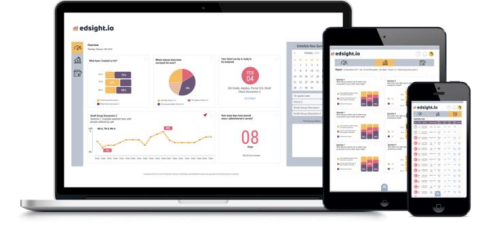
\includegraphics[width=1\linewidth]{figures/requirements-specification/Edsight-Dashboard-1.png}
    \caption{“Overview,” “Report,” and “Activity List” modes, displayed in desktop, tablet, and phone screens.}
    \label{fig: Edsight Dashboard 1}
\end{figure}

The report is the main dashboard in Edsight, where teachers can select filters such as date and classroom for display. Once a filter is applied, different results are displayed.


\begin{figure}[H]
    \centering
    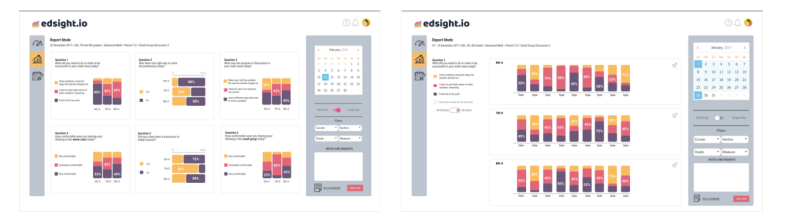
\includegraphics[width=1\linewidth]{figures/requirements-specification/Edsight-Dashboard-2.png}
    \caption{Edsight: (L) a single-event report with filters; (R) the multi-day comparison view.}
    \label{fig: Edsight Dashboard 2}
\end{figure}

Most current approaches to the learning dashboard do not live in lab sessions, as there is more course-level monitoring than session-level monitoring \cite{klerkx_2017_learning,verbert_2013_learning,ahn_2019_the}. This also has many benefits, helping students on the spot and allowing them to get the most out of their computer labs \cite{ahn_2019_the}.

\subsubsection{Real-Time Data Analytics and Visualisation}

Real-time analytics refers to the practice of collecting and analysing data as it is generated, with minimal latency between data collection and analysis \cite{marr_2021_what}. When we can process data as it comes in, we can gain insight and understand what is happening within a relevant context almost instantly. Such a practice is used in applications where data timeliness is critical, such as smart pricing and predictive maintenance \cite{marr_2021_what}. Traditional data analysis, where data is captured and stored, and insights are pushed out of storage. In contrast, real-time data analysis allows data to be analysed in real time. Real-time data analytics have proven to be highly valuable, as evidenced by the success of Netflix, which has perfected the art of predicting its customers' next favourite show \cite{marr_2021_what}.

Real-time analytics has emerged as a pivotal tool across multiple sectors, including retail, revolutionising decision-making processes and operational strategies \cite{mustafaayobamiraji_2024_realtime}. Retail giants such as Walmart and Amazon have leveraged real-time data analytics to personalise marketing campaigns, optimise pricing strategy, and efficiently manage inventory \cite{mustafaayobamiraji_2024_realtime}. Technologies such as RFID, IoT, and advanced analytics platforms were used to gather real-time data, analyse customer behaviour, and make data-driven decisions \cite{mustafaayobamiraji_2024_realtime}. A less utilised but more relevant application is in education, for example, a real-time machine learning application that detects learners' attention levels and participation using sensory data. The data allows teachers to recalibrate their teaching as necessary \cite{montebello_assisting}.

\begin{figure}[H]
    \centering
    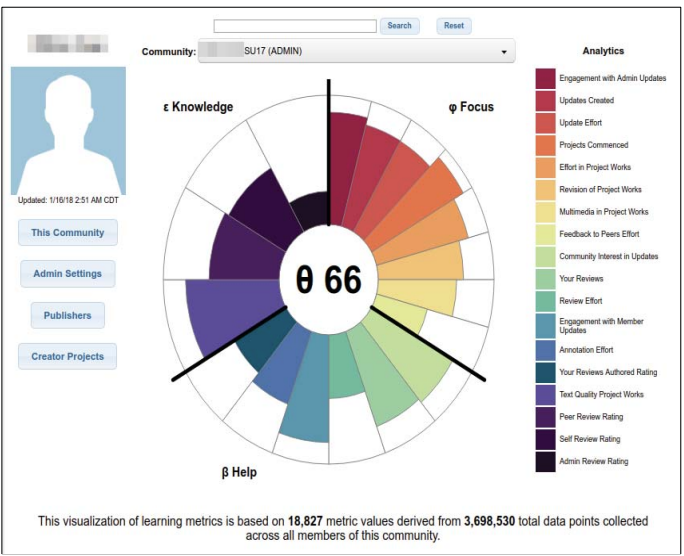
\includegraphics[width=1\linewidth]{figures/requirements-specification/Attention-Dashboard.png}
    \caption{The Learning Analytics Interface for a dashboard which collects data based on student attention}
    \label{fig: Attention Dashboard}
\end{figure}

Applying real-time analytics in computer labs will prove to be very beneficial for students and teachers alike. By collecting and processing data as it comes in, we will be able to update dashboards in real time and provide teachers with the most up-to-date information, enabling relevant, timely support. This would be better than a traditional data analysis approach, in which we review the data after the lab has finished, because our findings may not be relevant by then \cite{montebello_assisting,mustafaayobamiraji_2024_realtime}.

\subsection{Modelling Student Behaviour}

This section reviews how observable lab behaviour is modelled. 
It covers four themes in this area: detecting student struggle in the moment, tracing the growth of skill mastery over time, estimating which questions are hardest for the class, and training the composite signals that combine these. 
Student struggle and question difficulty are treated as complementary targets throughout: one identifies who needs help, the other identifies what the class as a whole finds hardest.


\subsubsection{Modelling Student Struggle}
A key challenge in supporting students during lab sessions is identifying which students are struggling and may require timely intervention. 
Studies in education have approached struggle detection at different temporal scales, ranging from within-assignment detection to course-level.
Dong et al.\ highlighted an approach that detects moments of struggle during a session based on time spent and progress relative to peers, achieving over 77\% accuracy when validated against expert judgement on whether intervention was needed \cite{dong_using}.
Struggle has been operationalised as failing the same unit test consecutively for more than four submission events, providing a clear threshold-based criterion \cite{dong_using}.

Beyond threshold-based approaches, more sophisticated methods have been explored. 
In related work, Or examined novice programmers' testing behaviour as an early step toward defining coding struggle, identifying patterns such as repeatedly submitting the incorrect answer for more than four submission events, signalling that students have stopped making meaningful progress \cite{or_2024_exploring,beckWheelSpinningStudentsWho2013}.
To move this even further, Estey et al.\ proposed a trajectory metric that measures changes in programming behaviour over time across a four-semester study of 514 students \cite{estey_2017_automatically}. 
Their early predictor identified 81\% of students who struggled throughout the course, but also flagged 43\% who went on to succeed, highlighting the difficulty of distinguishing slight from serious struggle.
Their trajectory metric reduced this false-positive rate to 11\%, demonstrating the importance of tracking how performance changes rather than measuring the students' current level \cite{estey_2017_automatically}.

Another approach uses machine learning to build a graphical model of how students navigate through programming assignments. By capturing the full solution trajectory, Piech et al.\ showed that a student's progression path is predictive of later difficulty, motivating the inclusion of the student's trajectory to track changes in answer quality across submissions \cite{piech_modeling}.

A complementary approach is knowledge tracing which models how a student's mastery of underlying skills progresses over time and it is examined in the next subsection.

Recent work on Large Language Models (LLMs) is also relevant as AI-generated feedback can provide more valuable insights than raw correctness alone.
Koutcheme et al.\ show that language models LLMs that are better at helping repair student programs also provide better explanations of coding issues, suggesting that the quality of LLM feedback can be studied empirically rather than assumed \cite{koutcheme_using}
More broadly, Pitts et al.\ survey LLM-based applications in programming education and argue that these systems are most effective when combined with human oversight rather than fully autonomous replacements \cite{pitts_a}

Together, these works demonstrate different methods for evaluating struggle. These metrics are best captured through a combination of temporal, correctness-based and behavioural signals.

\subsubsection{Knowledge Tracing and Bayesian Student Models}
A related but distinct line of work is knowledge tracing, which models how a student's mastery of underlying skills progresses over time.
Bayesian Knowledge Tracing (BKT) remains attractive because it is interpretable and computationally manageable.
Khajah shows that BKT can gain a performance boost by merging it with Item Response Theory (IRT) to model multidimensional problem difficulties and student abilities, without fitting student specific parameters, allowing the model to be generalisable to new students \cite{khajah_supercharging}.
In programming education, Kim et al.\ propose a knowledge tracing approach that integrates students' questions and automatically extracted skill information, showing that textual interaction data can provide useful signals about understanding misconception patterns \cite{kim_knowledge}.
This is relevant to the current project, as it suggests that struggles during computer labs should not be treated solely as repeated failures but also as informed by temporal behaviour, how the student develops, and question-specific context.  

Bayesian Knowledge Tracing was formalised by Corbett and Anderson in the context of an intelligent programming tutor, which treats the student's knowledge of each skill as either in a learned state or an unlearned state that can transition from unlearned to learned based on the student's interactions \cite{corbettKnowledgeTracingModeling1995}.
The model is governed by four interpretable parameters: an initial-learning probability, $p(L_0)$, an acquisition probability, $p(T)$ that a skill transitions from unlearned to learned at each practice opportunity, a guess probability, $p(G)$ for correct responses without mastery and a slip probability, $p(S)$ for incorrect responses despite mastery. The probability of a correct response on the next opportunity is then 
\begin{equation}
    p(C) = p(L) \cdot (1 - p(S)) + (1 - p(L)) \cdot p(G),
    \label{eq:bkt-prediction}
\end{equation} 
where $p(L)$ is the current estimate of mastery \cite{corbettKnowledgeTracingModeling1995}.
Here $p(L_0)$ is the prior probability of mastery before any attempt, whereas $p(L)$ is the running estimate after each observed response, updated by Bayes' rule and advanced by the transition $p(T)$; the full update is given in Section~\ref{sec: bkt}.
The original formulation assumes no forgetting, so the latent state cannot transition from learned back to unlearned.

Yudelson et al.\ extended BKT by individualising parameters across students and showed across KDD datasets that this yielded tangible improvements when predicting unseen student data \cite{yudelsonIndividualizedBayesianKnowledge2013}. They found that individualising the speed of learning $p(T)$ produced consistent gains in predictive accuracy, while individualising the prior $p(L_0)$ alone had no measurable effect, suggesting learning rate is the more important axis of student variation for BKT to exploit.

More recent work has explored neural alternatives to BKT such as deep learning approaches. Piech et al.\ proposed Deep Knowledge Tracing (DKT),  with two different types of Recurrent Neural Networks (RNNs): a Long Short Term Memory (LSTM) based model and a vanilla RNN model with sigmoid unit. These models predict a student's future performance based on their past activity. This resulted in a 25\% gain in the area under the curve (AUC) over the best previous result on a knowledge tracing benchmark as well as showing that knowledge tracing models do not need expert annotations \cite{piechDeepKnowledgeTracing2015}.
However, Khajah et al.\ subsequently showed that BKT extended with forgetting, latent student abilities, and automatic skill discovery matches DKT performance on average across four different data sets, arguing that the gains of deep approaches stem from added flexibility rather than from any representation discovery \cite{khajahHowDeepKnowledge2016}.
For an instructor facing dashboard, where the interpretability of mastery estimates is essential, BKT remains a defensible choice.

\subsubsection{Modelling Task Difficulty}


Alongside students' struggles, it is important to identify which questions pose the greatest difficulty for the class as a whole so that teachers can address the problem in front of the whole class rather than just for the student.
Dannath et al. examined task-level struggle detection methods in intelligent tutoring systems for programming, noting that prior work focused on dropout prevention rather than understanding the student's path towards the correct solution for a specific task \cite{dannath_evaluating}.
The separation in modelling is important as students may appear to be struggling with a genuinely difficult question rather than with individual performance. 
Additionally, if most of the class is struggling with a problem, it will be faster to go through the question with the whole class.

Task difficulty can be inferred from indicators such as failure rate, average time spent, number of attempts and the amount of feedback used before reaching a correct answer \cite{dannath_evaluating,piech_modeling}.
These measures are useful as they are directly observable and can be updated during a live session with low cost, but they do not separate question difficulty from variation in student ability.

Alternatively, we can model difficulty using Item Response Theory (IRT), which offers a more principled approach by accounting for how difficult a question actually is, rather than raw counts, as well as a student's latent ability \cite{rasch1960probabilistic,lord1968statistical}. It is worth noting that IRT captures how difficult a question is from the way students respond to it, which is not always the same as how hard the question is to learn or teach.
Baucks et al.\ uses IRT to analyse course difficulty variation and show how applying latent variable models can uncover meaning patterns in course rigor that is hidden when relying on simple metrics \cite{frederikbaucks_2024_gaining}. 
In online learning environments that allow multiple attempts, Pankiewicz argues that measuring task difficulty becomes more complex because task difficulty and feedback shape how it should be interpreted, motivating methods that go beyond raw metrics. \cite{pankiewicz_measuring}  
These works support the view that question difficulty should be modelled separately from student struggle and, where possible, that composite measures should be used rather than a single measure.

Overall, the literature suggests that task difficulty should be deduced from a combination of correctness, time, attempts, and progression-related information rather than from a single descriptive statistic \cite{dannath_evaluating,piech_modeling}.


\subsubsection{Composite Model Training and Optimisation}

Supervised learning allows us to refine composite weights through methods such as ordinary least squares (OLS) regression \cite{hastieElementsStatisticalLearning2009} or gradient boosting against externally-collected labels.
This method serves as an alternative to hand-set or manually tuned weights.
The supervised approach does not need to be human annotated as we can now leverage LLMs as raters; recent studies demonstrate substantial agreement with human annotators on classification tasks at a small cost and saving time \cite{gilardiChatGPTOutperformsCrowd2023, chiangCanLargeLanguage2023, zhengJudgingLLMasaJudgeMTBench2023, liuGEvalNLGEvaluation2023}.
Rather than tuning hyperparameters manually we can use modern Bayesian optimisation libraries such as Optuna's Tree-structured Parzen Estimator (TPE) to efficiently search the hyperparameter space and tune the scalar hyperparameters that govern these composite models \cite{NIPS2011_86e8f7ab, akibaOptunaNextgenerationHyperparameter2019}, as TPE produces stable optima in fewer iterations than other methods such as grid search and random search.

\subsection{Data-Driven Personalisation}

This section examines two data-driven techniques that move beyond scoring each student in isolation. 
Collaborative filtering infers a student's likely need for help from peers with similar interaction profiles, while text mining recovers the common mistake patterns hidden in free-text answers across the cohort. 
The two are complementary: one personalises at the level of the individual learner, the other surfaces structure shared across the class.



\subsubsection{Collaborative Filtering}

Beyond parametric approaches discussed in the previous subsection, more sophisticated data-driven methods have been explored in the educational recommender systems literature \cite{dasilva_2022_a, deschnes_2020_recommender}.
Collaborative filtering is an alternative method used for personalising user experiences \cite{resnickGroupLensOpenArchitecture1994}.
Unlike methods that rely on parameters, Collaborative filtering leverages the collective behaviour of users with similar histories to create preferences, on the principle that users with similar histories share similar needs \cite{schafer_2007_collaborative}. This method has been applied primarily in educational contexts to provide more efficient and accurate course suggestions than traditional methods \cite{li_2020_course}. This can be done with different types of models, such as linear regression and factor decomposers. It is evident that integrating intelligent recommendation technology significantly enhances resource utilisation and the overall student learning experience

A user-based collaborative filtering method identifies a set of $k$ nearest neighbours for a given student based on a similarity measure over their profiles \cite{herlockerAlgorithmicFrameworkPerforming1999}. The behaviour of the neighbours are aggregated to produce a prediction. The approach is shown to be effective in sparse datasets, where explicit ratings are unavailable and implicit signals such as time-on-task and submission frequency must serve as proxies for preference. A known limitation is that when a student has little interaction history, similarity cannot be computed reliably, leading to unstable early-session predictions.

In the context of lab struggle detection, collaborative filtering offers a strong alternative to our scoring approach. Rather than computing a fixed weighted score for each student, it can identify students whose interaction patterns closely resemble peers who need help, inferring that they too may need help. However applying collaborative filtering to a live computer lab comes with its constraints as students who may need help is limited and the start of the session will have very limited data. These constraints backs the use of a scoring approach, whilst the collaborative filtering approach is a strong alternative.


\subsubsection{Text Mining and Mistake Pattern Recovery} \label{sec: text mining}

Where student responses are free-text rather than numerical or categorical,
 identifying common mistake patterns requires text-mining techniques that combine information retrieval and unsupervised clustering.
Salton et al.\ introduced the vector space model for information retrieval, which represents documents and queries as vectors in a vector space, allowing for the computation of similarity between them \cite{saltonVectorSpaceModel1975}.
The standard weighting scheme is term frequency-inverse document frequency (TF-IDF) formalised in modern information retrieval as
\begin{equation}
    \mathrm{tf-idf}_{t, d} = \mathrm{tf}_{t, d} \cdot \log\frac{N}{\mathrm{df}_t},
    \label{eq:tfidf}
\end{equation}
where $\mathrm{tf}_{t, d}$ is the frequency of term $t$ in document $d$, $N$ is the total number of documents, and $\mathrm{df}_t$ is the number of documents containing term $t$ \cite{manningIntroductionInformationRetrieval2006}.

Once each document is represented as a TF-IDF vector, similar documents can be partitioned into clusters that share characteristic content.
MacQueen's $k$-means algorithm partitions $n$ points into $k$ clusters to minimise within cluster variance
\cite{MacQueen1967SomeMF}. 
Formally, this corresponds to choosing $k$ centres $C$ that minimise the sum of squared distances from each point to its closest centre,
\begin{equation}
    \phi = \sum_{x \in X} \min_{c \in C} \|x - c\|^2,
    \label{eq:kmeans}
\end{equation}
where $X$ is the set of data points \cite{arthurKmeansAdvantagesCareful}.
Because this objective is non-convex and sensitive to initialisation, Arthur and Vassilvitskii's $k$-means++ seeds initial centres by selecting each new centre with probability proportional to its squared distance from the nearest already-chosen centre, yielding provable approximation guarantees and faster convergence in practice \cite{arthurKmeansAdvantagesCareful}.

Choosing the number of clusters $k$ is itself a problem. Rousseeuw's silhouette coefficient quantifies how well each point fits its assigned cluster relative to the next-nearest cluster:
\begin{equation}
    s(i) = \frac{b(i) - a(i)}{\max\{a(i), b(i)\}},
    \label{eq:silhouette}
\end{equation}
where $a(i)$ is the mean intra-cluster distance for point $i$ and $b(i)$ is the mean distance from $i$ to all points in the nearest other cluster, with values close to $+1$ indicating tight well separated clusters \cite{rousseeuwSilhouettesGraphicalAid1987}. 
Sweeping $k$ and selecting the value that maximises the mean silhouette gives a principled auto-selection rule.
Once clusters are formed, a large language model can produce natural-language cluster explanations \cite{wangGoalDrivenExplainableClustering2023}.

\subsection{Retrieval-Augmented Feedback}
This section reviews the techniques that allow LLM feedback to be trusted in an educational setting. 
The central concern is hallucination: a model that generates fluent but unverified text can mislead a student who cannot yet judge its correctness. 
Retrieval-augmented generation addresses this by grounding the model's output in retrieved source material, and the subsections that follow cover both the generation step, the dense-embedding and approximate-nearest-neighbour retrieval that supplies it.




\subsubsection{Retrieval-Augmented Generation}

Lewis et al.\ introduced Retrieval-Augmented Generation (RAG) as a way to combine parametric language models with a non-parametric retriever over an external source, allowing the generator to condition its output on relevant evidence retrieved at query time \cite{lewisRetrievalAugmentedGenerationKnowledgeIntensive2020}.
 Additionally, RAG models hallucinate less and generate factually more correct text than BART \cite{lewisRetrievalAugmentedGenerationKnowledgeIntensive2020}.
Lewis et al.\ showed that RAG outperformed parametric models on knowledge intensive tasks, including open-domain QA tasks  \cite{lewisRetrievalAugmentedGenerationKnowledgeIntensive2020}.

In educational contexts, the case for retrieval is even stronger. 
Kasneci et al.\ survey the opportunities and challenges of large language models in education, noting that there is a difficulty in distinguishing between real knowledge and convincingly written but unverified model output due to the ability of LLMs to generate human-like text which can make it difficult for students to distinguish between real knowledge and unverified model output leading students to accept false or misleading information as true. 
To mitigate this risk, it is recommended we provide education on how information can be evaluated critically and teach students exploration, investigation, verification and corroboration strategies \cite{kasneciChatGPTGoodOpportunities2023}.
Retrieval-augmented generation can help mitigate this risk by grounding the model's output in verifiable sources, allowing students to trace the information back to its origin and evaluate its credibility \cite{lewisRetrievalAugmentedGenerationKnowledgeIntensive2020,kasneciChatGPTGoodOpportunities2023}.

\subsubsection{Dense Retrieval and Approximate Nearest Neighbour Search}

Before the retrieval step in RAG, we need a representation that captures semantic similarity between documents and queries.
Reimers and Gurevych proposed Sentence-BERT (SBERT), which is a modification of pre-trained BERT that uses siamese and triplet network structures to derive semantically meaningful sentence embeddings that can be compared using cosine similarity \cite{reimersSentenceBERTSentenceEmbeddings2019}.
In the paper they show that commonly used approaches to derive sentence embeddings from BERT such as CLS-token outputs or averaging the BERT output embeddings perform worse than averaged GloVe embeddings on standard semantic textual similarity benchmarks. Siamese fine-tuning on natural language inference data substantially improves correlation on STS benchmarks and outperforms sentence-embedding methods such as InferSent and Universal Sentence Encoder \cite{reimersSentenceBERTSentenceEmbeddings2019}.

Once documents are embedded, exact nearest neighbour search scales linearly with the number of documents which is unfeasible for large retrieval over large collections.
To relax this, Approximate Nearest Neighbours Search (K-ANNS) was proposed, which relaxes the condition of the exact search by allowing a small number of errors in exchange for faster than linear time complexity \cite{malkovEfficientRobustApproximate2016}.
Malkov and Yashunin proposed Hierarchical Navigable Small World (HNSW) graphs, which are a fully graph based ANN index that incrementally builds a multi-layer structure of proximity graphs for nested subsets of the stored elements \cite{malkovEfficientRobustApproximate2016}.
As queries descend greedily from top to the zero layer, logarithmic complexity is achieved, with the evaluation showing that HNSW outperforms previous open source vector only approaches \cite{malkovEfficientRobustApproximate2016}.

Together retrieval-augmented generation, dense sentence embeddings, and approximate nearest neighbour search build the standard pipeline for grounding LLM output.

\subsection{Existing Systems}

This section surveys systems already deployed in education to locate where the present work sits. 
It reviews learning management systems, instructor-facing dashboards, early-warning systems for at-risk students, and the recent class of real-time classroom support systems that sits closest to this work. 
The first three operate largely at the level of the course and review data after the fact; the last bring analytics into the live session, and it is against these that the present contribution must be positioned.

\subsubsection{Learning Management System }
A learning management system administers, tracks and delivers educational courses and materials \cite{wikipediacontributors_2019_learning_management_systems}; such systems hold the largest share of the learning-systems market, almost every higher-education institution has adopted one, and Moodle is the most widely used \cite{wikipediacontributors_2019_learning_management_systems}. They were designed to surface learning gaps through analytics but that reporting has two properties to address: it is reviewed after an activity has finished, so a student who struggled in a lab may already have left without timely help, and it is utilised at the level of the course. Course-level reporting is well suited to curriculum design and long-term planning but it is not suited to the live lab, where support is only useful before the student moves on. It is precisely this gap that the present work targets.

\subsubsection{Instructor Facing Dashboards}

Learning management systems often incorporate dashboards that visualise student progress so that teachers can locate knowledge gaps \cite{kiatxin_development}; the dashboard has become the central output of learning analytics. Existing examples such as Blocks: Progress Bar report active time, assignment progress, marks and submission counts \cite{kiatxin_development,holsteinIntelligentTutorsTeachers2017a,holsteinStudentLearningBenefits2018}. What they report, however, is how far a student has progressed, not whether a student is struggling, and they do so at the course level rather than the live session. This project keeps the dashboard format but pivots it from progress tracking towards real-time struggle and difficulty within the session itself.


\begin{figure}[H]
    \centering
    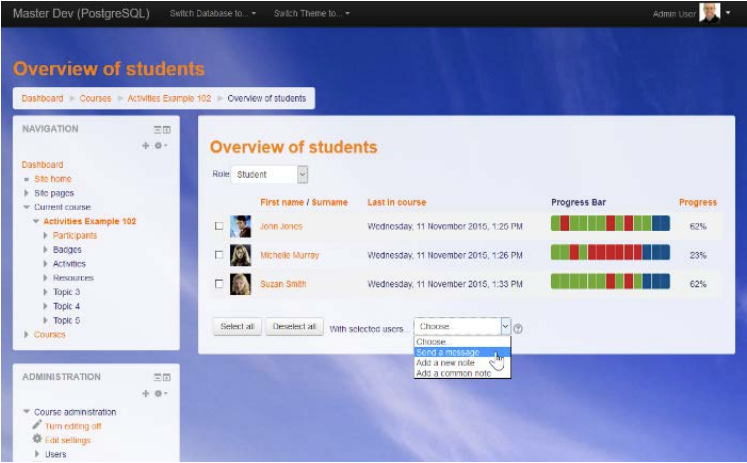
\includegraphics[width=1\linewidth]{figures/requirements-specification/Piwik-Analytics.png}
    \caption{Piwik Analytics}
    \label{fig: Piwik Analytics}
\end{figure}

Another implementation of a learning dashboard is the Multi-Modal (MM) teacher dashboard, the MM dashboard: 1) receives data from eye trackers, wristbands, web cameras, and the learning activity; 2) computes the student’s relevant cognitive, affective, and physiological measurements; 3) synchronises and visualises the resulting measurements in a clean, customisable interface; and 4) notifies instructors during potential moments of interest \cite{leecultura_2023_multimodal}.
\begin{figure}[H]
    \centering/u
    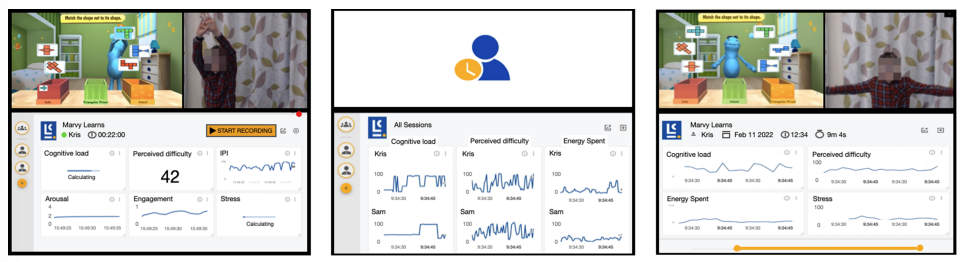
\includegraphics[width=1\linewidth]{figures/requirements-specification/MM-Dashboard.png}
    \caption{Different views of MM dashboard: SSV (left), ASV (centre), and RSV (right).}
    \label{fig: MM dashboard}
\end{figure}
The MM dashboard has three ways of data visualisation, as we can see in \ref{fig: MM dashboard}: 1) single session view (SSV), which displays real-time learning data from a single student’s session; 2) all sessions view (ASV), which shows real-time learning data from all connected students; and 3) replay session view (RSV), which allows the teacher to interact with previously recorded session data from a single student session \cite{leecultura_2023_multimodal}. The views are divided into panels, and we can also see that the SSV and ASV have a right-side navbar used to switch between panels \cite{leecultura_2023_multimodal}.

However, the dashboards do come with a range of issues. For the MM dashboard to work, students must have a range of sensors, which are uncommon for them \cite{leecultura_2023_multimodal}. Teachers also report no experience with some of the hardware required for the MM dashboard to work. Although this is a key problem, it was not the MM dashboard's main issue; the main issue was that teachers may lack the knowledge to understand and interpret the dashboard results, as the majority of users reported unfamiliarity with the measurements provided. The importance of the metrics was also questioned \cite{leecultura_2023_multimodal}. The study also noted that hands-on training may be required to help teachers use the system efficiently \cite{leecultura_2023_multimodal}.

The limitations highlight a critical gap in the practicality and potential for utilisation of the learning dashboards. Whilst the dashboards provide high-level insights, many of these insights are difficult to understand, prompting educators to question their importance. Also, these dashboards tend to be unintuitive, which can be especially an issue for educators who are not STEM-oriented. We can leverage these insights to create clearer indicators, such as struggle, and by taking a more straightforward approach to the dashboard, we can address these gaps and create better, more useful learning dashboards.


\subsubsection{Early Warning and At-Risk Student Systems}

Early warning systems in education identify students at risk of poor learning outcomes by analysing routinely collected data and surface those students to instructors before failure becomes irreversible \cite{macfadyenMiningLMSData2010}.
In education, an At-risk student system is an early warning system that spots struggling students before it is too late \cite{baeres_2020_an}. 
Recently, many approaches to at-risk student systems have leveraged AI to identify students at risk \cite{baeres_2020_an}.


Student data is analysed to flag potential issues. Typically, grades, attendance, online activity, and behaviour are used to alert teachers to help students early, before problems grow \cite{baeres_2020_an}. The datafication of education enables the use of automated methods to detect patterns in extensive educational data. Approaches leverage predictive models to use the data, predicting the likelihood that a student will fail a course \cite{baeres_2020_an}.

We can look at the edInsight Early Warning System as an example. This system looks at the course as a whole and uses the information gained to determine an at-risk ranking for all students \cite{a2020_atrisk}. The system leverages a scoring system, based on specific categories such as the Course grade category \cite{a2020_atrisk}:

\begin{table}[H]
    \centering
    \begin{tabular}{|c|c|}
        \hline
        Grade & Score\\
        \hline
        \hline
        C- & 2 \\
        \hline
        D+ & 4\\
        \hline
        D & 8\\
        \hline
        F & 10\\
        \hline
    \end{tabular}
    \caption{Grade-based scoring: lower grades raise the struggle score.}
    \label{tab: grade scoring}
\end{table}
With the scores calculated, educators have a clear idea of which students are most at risk, making this information useful for directing attention to those who need the most help \cite{a2020_atrisk}.
The same approach has been validated in academic environments. Arnold and Pistilli describe the Course Signals system at Purdue, which is an early intervention system that combines grade, past academic history and demographic predictors into a traffic light indicator for instructors, reporting measurable gains in student retention \cite{arnoldCourseSignalsPurdue2012a}.
Jayaprakash et al.\ generalises this further with an open-source initiative, the Open Academic Analytics Initiative (OAAI), which has been deployed across multiple US institutions, demonstrating that the underlying predictive techniques are not specific to a single platform \cite{jayaprakashEarlyAlertAcademically2014}.


Although the system is beneficial for identifying students who are struggling at the course level, it does not necessarily help identify students at the lab level, as its design assumptions do not align with the demands of lab sessions. Educators working in real-time sessions require live data. Hence, they have immediate awareness of which students are currently struggling, rather than future failure. However, we can apply the same concepts used in at-risk systems to identify students who are struggling the most and questions that have the most difficulty. As a result, as a result while traditional at risk systems are not designed for lab sessions, the underlying principles can be adapted to meet the needs of real-time lab analytics.


\subsubsection{Real-Time Classroom Support Systems}

The closest prior work brings analytics into the live programming session itself. Diana et al.\ present an instructor dashboard that predicts, from live program-state logs, which students need help during an interactive programming assignment \cite{dianaInstructorDashboardRealtime2017}; the same group separately matches low-performing students to higher-performing peer tutors. 
ClassAid moves into orchestration: it places a configurable tutoring agent alongside each student and gives the instructor a live dashboard to monitor the student-AI interaction and switch each agent between technical, heuristic, automatic and silent feedback modes \cite{zhangClassAidRealtimeInstructorAIStudent2026}. Both keep an instructor in the loop, yet neither derives a per-submission correctness signal, ranks question difficulty separately, or clusters the cohort's mistakes.

A related line of work delivers awareness through specialised hardware. 
Lumilo, a set of mixed-reality glasses, presents per-student detector states and Bayesian mastery estimates to a teacher, directing attention to the students who need it most without interrupting the class \cite{holsteinIntelligentTutorsTeachers2017a, holsteinStudentLearningBenefits2018}. The multi-modal teacher dashboard described pursues the same goal through eye-trackers, wristbands and cameras \cite{leecultura_2023_multimodal}. These systems show that real-time awareness is valuable, but they are dependent on the use of certain hardware which may be inaccessible and some stop at awareness rather than routing a person to the student.

A meta-analysis of classroom orchestration systems finds that teacher awareness is the function most strongly associated with improved outcomes, yet awareness on its own does not direct help to where it is needed \cite{fengEffectivenessFunctionsClassroom2023}. Each system above provides one or two of the capabilities this project brings together, but none unites an automatically-derived per-submission correctness signal, separate rankings of student struggle and question difficulty, live clustering of cohort mistakes, and the dispatch of a human assistant over a mobile channel. Table~\ref{tab:rt-systems} summarises how these systems compare with the current project.

\begin{table}[H]
\centering
\small
\setlength{\tabcolsep}{4pt}
\begin{tabular}{|l|c|l|c|c|l|l|}
\hline
System (year) & Live & Signal source & Strug. & Diff. & Dispatch & Device \\
\hline\hline
\textbf{This work} & Y & logs + LLM correctness & Y & Y & human assistant & mobile \\
\hline
Diana (2017) & Y & program-state logs & Y & N & peer (separate) & desktop \\
\hline
ClassAid (2026) & Y & LLM + interaction & part. & N & AI agent & desktop \\
\hline
Lumilo (2018) & Y & ITS detectors + BKT & part. & N & awareness & MR glasses \\
\hline
MM dashboard (2023) & Y & physiological sensors & part. & N & awareness & desktop \\
\hline
\end{tabular}
\caption{Real-time classroom support systems compared with the developed system in this report}
\label{tab:rt-systems}
\end{table}


\subsection{Research Gaps}

This subsection reviewed a range of relevant literature. Learning analytics has proved incredibly useful in higher education by providing data on MOOC completion rates, click counts, and time spent, which have significantly aided pedagogical decision-making. Learning dashboards have also emerged as the primary output of learning analytics, enabling educators to gain insight into how different students are performing through an intuitive user interface. Real-time analytics has enabled processing data as it arrives, benefiting multiple sectors. 
The review also examined the methods that can turn this data into actionable signals: struggle detection, knowledge tracing and Bayesian student models, item-response and composite approaches to question difficulty, collaborative filtering, text mining for mistake-pattern recovery, and retrieval-augmented generation for grounded feedback. 
Each of these have been well established on their own, the gap this thesis addresses lie at their intersection, in the setting of a live computer lab session. 
While the systems reviewed above show that real-time dashboards and classroom orchestration tools exist, a systematic review finds that learning analytics dashboards have not reliably improved student achievement \cite{kaliisaHaveLearningAnalytics2024}; the contribution therefore lies not in another visualisation, but in integrating these signals and acting on them within the session.

In particular, computer labs face a distinct challenge that existing approaches don't address well. In these settings, teachers and assistants have no way to swiftly identify those who need help and must rely on those who put their hands up. The problem with this is that it does not account for shy students who may not want to put their hands up, causing them to spend too much time on a question. Also, current dashboards focus on data collected towards the end of the lab; this data may not be as valid afterwards. 
A dashboard built on real-time analytics addresses this issue directly by leveraging the data as it is generated to support students during the session itself, rather than after it, when intervention is no longer possible.

Three gaps emerge from the work on signals and detection. 
First, LLMs have been studied as a source of explanatory feedback \cite{koutcheme_using, pitts_a} and, in orchestration systems, as tutoring agents dispatched to the student \cite{zhangClassAidRealtimeInstructorAIStudent2026}, but not as a live correctness signal which combines metrics such as correctness, attempt amount and time into a struggle score. 
Where LLMs have instead been asked to judge difficulty directly they align poorly with human-perceived difficulty \cite{liCanLLMsEstimate2025, tabibTrustworthyDifficultyAssessments2025}, which motivates combining the model's signal with item-response and Bayesian estimates rather than relying on it alone.
Second, struggle detection operates largely at the course level \cite{estey_2017_automatically}, and where it is applied within a session it rests on simple threshold rules, such as four consecutive failed submissions \cite{dong_using}, which capture only one of the several factors, time, attempts, trajectory and answer quality, that signal difficulty. 
Third, collaborative filtering is well established for course recommendation \cite{li_2020_course, schafer_2007_collaborative}, yet its use for real-time lab struggle detection is unaddressed, in part because the sparsity of data at the start of a session makes similarity hard to compute reliably \cite{herlockerAlgorithmicFrameworkPerforming1999}.

Two further gaps address understanding the cohort as a whole. Bayesian Knowledge Tracing has been used to estimate the mastery of individual students \cite{corbettKnowledgeTracingModeling1995, yudelsonIndividualizedBayesianKnowledge2013}, but not to give an instructor a view of where a live session's student's mastery sits across the skills a session exercises. Similarly, text mining and clustering are well developed for organising document collections \cite{saltonVectorSpaceModel1975, MacQueen1967SomeMF}, yet they have not been applied to the free-text answers of a live session to surface the common mistakes the class is making, so that an instructor can address them once for everyone. 
A related gap concerns trust in any feedback the system offers: LLM output in education is prone to convincing yet unverified hallucination \cite{kasneciChatGPTGoodOpportunities2023} and retrieval-augemented generation can ground that output in course material \cite{lewisRetrievalAugmentedGenerationKnowledgeIntensive2020}, but this grounding has not been built into a live lab tool that suggests feedback to assistants and instructors to aid students.

Finally the delivery of this information to those who act on it is a critical gap. 
Existing dashboards present analytics on a screen but offer no channel that sends information on how to aid students to lab assistants as they circulate the room. 
This motivates a mobile assistant view that delivers allocations and suggested help on an assistant's own device. 
Mixed-reality displays for teacher awareness already exist \cite{holsteinStudentLearningBenefits2018}, so the contribution here is not the hardware but a more accessible system that needs no per-student sensors or instrumented tutoring system, together with the development of an accurate model for assessing student struggle and question difficulty; the system keeps the human in the loop that the evidence favours over fully automated support \cite{pitts_a}, and heavier wearable integration such as smartwatches or glasses is left to future work.



Taken together these gaps point to a clear opportunity for a real-time, session-level dashboard that combines multi-signal measures of struggle and difficulty, an AI-derived correctness signal, a cohort view of common mistakes, grounded LLM suggestions for how to help, and a lightweight channel for dispatching that generated feedback to roaming assistants. No existing system brings these together for the live computer lab. Providing this system and evaluating how well its signals agree with expert judgement, is the contribution of this thesis.

\subsection{Requirements Specification}

This section specifies what the system must do, drawing on the gaps identified above. It sets out the functional requirements, the non-functional requirements that constrain how they are met, and a MoSCoW prioritisation that orders them for a single-developer project.

\subsubsection{Functional Requirements}
In this section, we define the core functionality required of the proposed system to address the problem in Chapter \ref{sec: intro} and the gaps highlighted earlier. These requirements specify what the system must do regardless of implementation.

\paragraph{FR1: Live ingestion of Lab data}
The system must be capable of ingesting student interaction data as it is generated in the lab sessions, which includes data which is produced whilst students are answering questions, such as attempts amount, how wrong the answer is, how long spent on the question, which will be used for measuring student struggle as well as metrics we will use in measuring question difficulty such as total attempt amount, total correct submissions and average time spent.

\paragraph{FR2: Computation of student struggle}
The system must compute a metric to represent how much a student is struggling in labs, derived from data highlighted in \textbf{FR1}. This representation should represent short-term difficulty rather than long-term ability and predicted outcomes.

\paragraph{FR3: Computation of  question difficulty}
The system must compute a metric for question difficulty used to represent how hard a question or task is in a lab session, derived from the data highlighted in \textbf{FR1}. This will represent a task that is difficult for everyone in attendance at the lab.

\paragraph{FR4: Real-time prioritisation}
The system must provide an indicator of which students are struggling most in computer labs, based on student struggle data, allowing instructors to aid those who need it most.

\paragraph{FR5: Present Relevant Analytics}
The system must present relevant analytics for the labs in a suitable, intuitive form that can be interpreted quickly to enable quick decision-making.

\paragraph{FR6: Smart Device}
The system must integrate with smart devices such as phones, watches and glasses, in particular the smartphones so that information can be sent swiftly to lab assistants.

\paragraph{FR7: Lab Assistant Ranking System}
The system will record and display lab assistant contributions during the session so that assistant activity can be monitored and incentivised.

\subsubsection{Non-Functional Requirements}
In addition to functional requirements, the system must satisfy non-functional requirements to ensure the system operates as intended. These requirements reflect the practical constraints of the live lab sessions and ensure efficient operation.

\paragraph{NFR1: Real Time Performance }
The system must process and update analytics with minimal latency to support swift decision-making in lab sessions. Delays should not prevent an instructor from responding to students who need help.

\paragraph{NFR2: Interpretability}
Outputs should be interpretable by instructors without requiring specialist knowledge or extensive training. The system should be intuitive so that it can be used across all educational disciplines. Analytics should aid in understanding rather than providing overly complex information.

\paragraph{NFR3: Robustness to noisy data}
The presence of noisy or incomplete data should not interfere with the system's operations. Noisy or incomplete data should be accounted for and not interfere with the provision of correct analytics.

\paragraph{NFR4: Scalability}
The system should be capable of operating efficiently in various labs regardless of module, class size and question type.

\paragraph{NFR5: Privacy and Ethical}
Data must be handled responsibly and solely for the purpose of providing analytics in computer labs, and it must not be used for any purpose other than aiding students.

\paragraph{NFR6: Extensibility and Maintainability}
The system must be designed to accommodate additional data sources or metrics without requiring a fundamental redesign, enabling future extensions.


\subsubsection{Requirements Prioritisation (MoSCoW)}
For this section, we will use a MoSCoW table to highlight the project's requirements prioritisation, reflecting on time constraints and the project scope.



\begin{table}[H]
    \centering
    \begin{tabular}{|p{0.2\textwidth}|p{0.2\textwidth}|p{0.2\textwidth}|p{0.4\textwidth}|}
        \hline
        Must Have & Should Have & Could Have & Won't Have \\
        \hline
        \hline
        FR1& FR5 & FR7 & Long term student outcomes\\
        \hline
        FR2& FR6 &  & Fully AI decision making\\
        \hline
        FR3& NFR3 &  & Avatar based AI assistance\\
        \hline
        FR4& NFR4 &  & \\
        \hline
        NFR1& NFR6 &  & \\
        \hline
        NFR2&  &  & \\
        \hline
        NFR5&  &  & \\
        \hline

    \end{tabular}
    \caption{MoSCoW table highlighting requirements for proposed software}
    \label{tab: MosCoW}
\end{table}



\section{Design and Modelling} \label{sec:design}
This section describes the design and architecture of the lab dashboard, highlighting how various components are implemented. It covers the data endpoint, defining what data enters the system and in what form, the mathematical models used to derive struggle and difficulty and the user interface design which exposes the analytics to educators. 
 
\subsection{System Architecture}

The proposed system adopts a layered architecture designed to support real-time learning analytics in computer lab environments. 
The architecture separates data generation, data ingestion and processing, as well as decision-making and action, into three distinct layers, ensuring each component can evolve independently. 

\begin{figure}[H]
    \centering
    \resizebox{\linewidth}{!}{%
    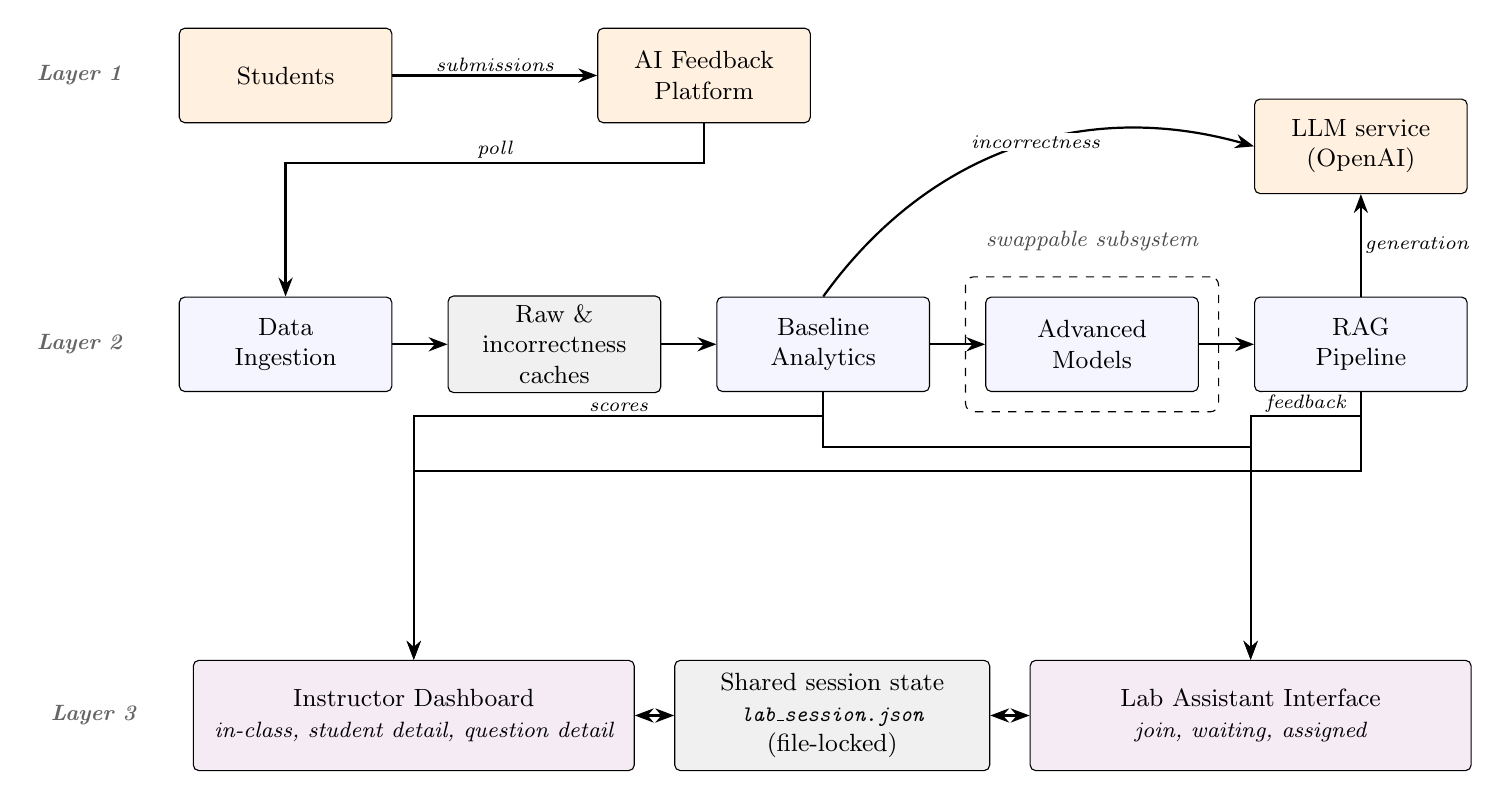
\begin{tikzpicture}[
        node distance = 0.9cm and 0.7cm,
        process/.style = {
            rectangle, draw, rounded corners=2pt,
            minimum width=2.7cm, minimum height=1.2cm,
            align=center, font=\small, fill=blue!4
        },
        store/.style = {
            rectangle, draw, rounded corners=2pt,
            minimum width=2.7cm, minimum height=1.2cm,
            align=center, font=\small, fill=gray!12
        },
        ui/.style = {
            rectangle, draw, rounded corners=2pt,
            minimum width=5.6cm, minimum height=1.4cm,
            align=center, font=\small, fill=violet!8
        },
        external/.style = {
            rectangle, draw, rounded corners=2pt,
            minimum width=2.7cm, minimum height=1.2cm,
            align=center, font=\small, fill=orange!12
        },
        flow/.style = {-{Stealth[length=2.4mm]}, thick},
        biflow/.style = {{Stealth[length=2.4mm]}-{Stealth[length=2.4mm]}, thick},
        grouplabel/.style = {font=\footnotesize\itshape, anchor=south, text=black!70},
        edgelabel/.style = {font=\scriptsize\itshape, fill=white, inner sep=1pt},
        layerlabel/.style = {font=\footnotesize\bfseries\itshape, anchor=east, text=black!60}
    ]
        % ===== Layer 1 - Data Generation =====
        \node[external] (students) {Students};
        \node[external, right=2.6cm of students] (endpoint) {AI Feedback\\Platform};
        \draw[flow] (students) -- node[edgelabel, above]{submissions} (endpoint);

        % ===== Layer 2 - Ingestion \& Processing =====
        \node[process, below=2.2cm of students] (ingest) {Data\\Ingestion};
        \node[store, right=of ingest] (caches) {Raw \&\\incorrectness\\caches};
        \node[process, right=of caches] (baseline) {Baseline\\Analytics};
        \node[process, right=of baseline] (advanced) {Advanced\\Models};
        \node[process, right=of advanced] (rag) {RAG\\Pipeline};

        % External LLM service, above the right end of the pipeline
        \node[external, above=1.3cm of rag] (llm) {LLM service\\(OpenAI)};

        % Dashed group around the swappable models cluster
        \begin{scope}[on background layer]
            \node[draw, dashed, rounded corners=3pt,
                  fit=(advanced),
                  inner sep=0.25cm] (modelgroup) {};
        \end{scope}
        \node[grouplabel] at (modelgroup.north) [yshift=2mm] {swappable subsystem};

        % Layer 2 internal flows
        \draw[flow] (endpoint.south) -- ++(0,-0.5) -| (ingest.north)
            node[edgelabel, pos=0.25, above]{poll};
        \draw[flow] (ingest) -- (caches);
        \draw[flow] (caches) -- (baseline);
        \draw[flow] (baseline) -- (advanced);
        \draw[flow] (advanced) -- (rag);
        \draw[flow] (baseline.north) to[bend left=35]
            node[edgelabel, pos=0.55]{incorrectness} (llm.west);
        \draw[flow] (rag.north) -- node[edgelabel, right]{generation} (llm.south);

        % ===== Layer 3 - Decision \& Action =====
        % Shared session state placed BETWEEN the two UIs so the file-locked
        % coordination between Instructor and Assistant is visually obvious.
        \node[ui, below=3.4cm of baseline, xshift=-5.2cm] (instructor)
            {Instructor Dashboard\\\footnotesize\itshape in-class, student detail, question detail};
        \node[store, right=0.5cm of instructor, minimum width=4.0cm, minimum height=1.4cm] (state)
            {Shared session state\\\footnotesize\itshape \texttt{lab\_session.json}\\(file-locked)};
        \node[ui, right=0.5cm of state] (assistant)
            {Lab Assistant Interface\\\footnotesize\itshape join, waiting, assigned};

        % Layer 2 -> Layer 3 flows (staggered bend depths per arrow to avoid shared horizontal channels)
        % Baseline -> Instructor (short L, near source)
        \draw[flow] (baseline.south) -- ++(0,-0.3) -|
            node[edgelabel, pos=0.25, above]{scores} (instructor.north);
        % Baseline -> Assistant (cross right, mid-depth bend)
        \draw[flow] (baseline.south) -- ++(0,-0.7) -| (assistant.north);

        % RAG -> Assistant (short L, near source)
        \draw[flow] (rag.south) -- ++(0,-0.3) -|
            node[edgelabel, pos=0.25, above]{feedback} (assistant.north);
        % RAG -> Instructor (cross far left, deepest bend)
        \draw[flow] (rag.south) -- ++(0,-1.0) -| (instructor.north);

        % Inter-UI coordination via file-locked shared session state (horizontal row)
        \draw[biflow] (instructor.east) -- (state.west);
        \draw[biflow] (state.east) -- (assistant.west);

        % Layer labels in the left margin
        \node[layerlabel] at ([xshift=-0.6cm]students.west) {Layer 1};
        \node[layerlabel] at ([xshift=-0.6cm]ingest.west) {Layer 2};
        \node[layerlabel] at ([xshift=-0.6cm]instructor.west) {Layer 3};
    \end{tikzpicture}}
    \caption{V2 system architecture: a three-layer pipeline from data ingestion through baseline and advanced analytics and the RAG pipeline to the instructor and lab-assistant surfaces, coordinated via the file-locked shared session state.}
    \label{fig: system architecture}
\end{figure}

\paragraph{Data Generation Layer}
As seen in Figure \ref{fig: system architecture}, student interactions form the primary source of data. When students submit an attempt or request feedback, the interaction data is recorded at the endpoint and not modified.

\paragraph{Data Ingestion and Processing Layer}
Data ingestion is performed periodically according to the user-defined refresh rate. Retrieved data will be stored in the raw data store, then parsed and normalised before being used for calculations. The data will be used to determine student struggle, question difficulty, and other required metrics.

\paragraph{Decision and Action Layer}
Data Analytics will now be sent to the learning dashboard for presentation to the instructor, thereby aiding decision-making. The instructor will identify students who are struggling. More complex questions will also be identified so that the instructor can go through the questions with the whole class. Instructors will use the dashboard to assign tasks to assistants to assist students who need help.

This layered design supports the project's aim of providing timely, targeted support during lab sessions while using the system as a decision-making tool for student support. Later sections build on this architecture.

\subsection{Data Endpoint} \label{sec: data endpoint}
A data endpoint is a specific URL or address in a web service or API that defines where and how clients can access the service. The proposed system integrates with the existing AI feedback platform through a single external data endpoint. The data endpoint is crucial in our system as it provides access to detailed records of student submissions and feedback interactions generated as students engage with lab questions. As outlined in Figure \ref{fig: system architecture}, the endpoint serves as the entry point to the analytics pipeline, supplying the raw data that will be processed, normalised, and aggregated for data visualisation. The integration is designed to be read-only, ensuring the data and metrics are not tampered with.

The endpoint returns an array in JSON format, where each record corresponds to a specific session based on the session's first submission time. Alongside standard fields such as module, question, timestamp and user, each record has an XML payload. The payload captures the interaction history for a given session, including submissions and AI responses. The design reflects the constraints of the existing system while providing vital information for our analytics.

Interaction data are organised around sessions, where a session represents a continuous period of student engagement from the first submission attempt. Within a session, students may have multiple submissions, getting multiple AI responses. This is beneficial in reflecting how their answers may improve question by question. The structure allows the capture of temporal patterns, repeated attempts, and help-seeking behaviour, which will be vital for identifying short-term struggle and difficult questions in lab sessions.

\begin{figure}[H]
    \centering
    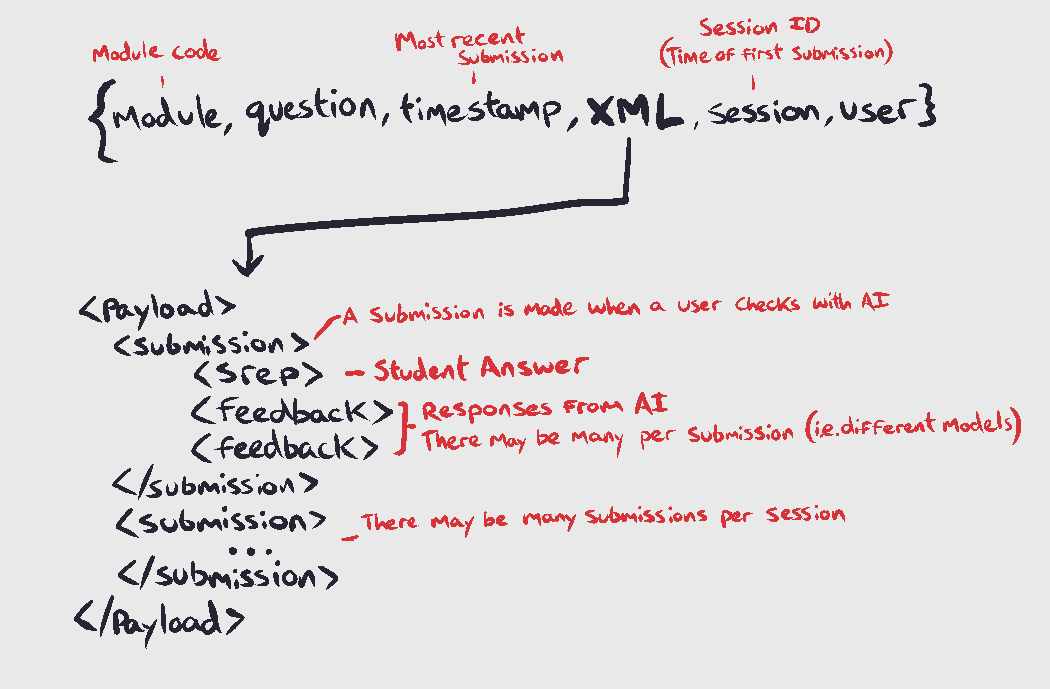
\includegraphics[width=1\linewidth]{figures/design-and-architecture/data-entry.png}
    \caption{Structure of session-based interaction data returned by feedback system}
    \label{fig: data entry}
\end{figure}

From the session-based data, the system derives a set of core metrics for real-time monitoring. These include attempts per question, time between attempts, AI-based indicators of correctness, and the frequency with which students request feedback. By using these, we will enable the system to distinguish among students and identify those who are struggling the most. The derived metrics will form the basis of our two key metrics: student struggle and question difficulty.

It is essential to consider that we may receive incomplete or noisy data during sessions, which could stem from students repeatedly returning to the AI feedback system or from procrastination on their work. Not all indicators of struggle and question difficulty are valuable on their own; hence, they are combined to produce indicators of student struggle and question difficulty.



\subsection{Baseline Analytics Design}
This section describes the baseline metrics, student struggle and question difficulty and the data from the endpoint that is used to derive them.
\subsubsection{Student Struggle Model} \label{sec: student struggle}

\paragraph{Modelling Objective}
To model student struggle, let $s$ denote a student and $\sigma$ denote the session. We will denote students who struggle with a scalar function:
\begin{equation}
    S(s,\sigma) \in [0,1]
\end{equation} \label{eq: scalar in range model}
The student struggle function will allow us to quantify the degree of difficulty that students $s$ are currently experiencing during session $\sigma$, based on the observable data from the endpoint in Section \ref{sec: data endpoint}. The model will support real-time prioritisation in computer labs.

\paragraph{Identified Variables}
From the session-based interaction data described in Section \ref{sec: data endpoint}. We can derive the following quantities:
\begin{itemize}
    \item $n_{s,\sigma}$ - The total number of submissions made by a student $s$ during session $\sigma$
    \item $t_{s,\sigma}$ - The total active time elapsed during session $\sigma$
    \item $i_{s,\sigma}$ - The average AI incorrectness measure for student $s$ during session $\sigma$, derived from AI-Based answer ratings
    \item $r_{s,\sigma}$ - The number of retry submissions within session $\sigma$
    \item $d_{s,\sigma}$ - The regression slope of incorrectness scores against the submission index, which captures whether a student is improving or deteriorating across the session
    \item $\mathrm{rep}_{s,\sigma}$ - The number of exact-match repeated submissions within session $\sigma$
\end{itemize}
By leveraging metrics linked to student struggle, we can produce a student struggle score

\paragraph{AI-Based Answer Rating}
Let $A_{s,\sigma,k}$ be the $k$-th submitted answer by student $s$ in session $\sigma$. We will derive an LLM-based scoring function. Where $Q_{\sigma}$ is the current question and $A_{\sigma}$ is the answer, we will define our LLM-based scoring function to be:
\begin{equation}
    c_{s,\sigma,k} = C(A_{s,\sigma,k},A_{\sigma},Q_{\sigma}) \in [0,1]
\end{equation}
where $c_{s,\sigma,k}$ is the correctness measure that measures the quality of a students answer, where 1 is the correct answer and 0 is completely wrong. We can then define our incorrectness measure:
\begin{equation}
    i_{s,\sigma,k} = 1 - c_{s,\sigma,k} \in [0,1]
\end{equation}

\paragraph{Normalisation}

The retry rate, repetition rate and trajectory slope are derived from the counts identified earlier:

\begin{equation*}
    \tilde{r}_{s,\sigma} = \frac{r_{s,\sigma}}{n_{s,\sigma}} \in [0,1], \qquad
    \tilde{\mathrm{rep}}_{s,\sigma} = \frac{\mathrm{rep}_{s,\sigma}}{n_{s,\sigma}} \in [0,1].
\end{equation*}

The trajectory slope $d_{s,\sigma}$ is signed (negative values indicate improvement, positive values indicate deterioration) and therefore unbounded by definition. The mean incorrectness $i_{s,\sigma}$ and the time decayed recent-incorrectness $A^{raw}(s,\sigma)$ are already bounded to $[0,1]$ by construction as each is an average of values already in $[0,1]$.

To ensure each component contributes the weighting intended, every signal is min-max normalised across the cohort for the session with:
\begin{equation*}
    \hat{x}_{s,\sigma}
    = \frac{x_{s,\sigma} - x_{\min}}{x_{\max} - x_{\min}},
    \qquad
    x_{\min} = \min_{s' \in S} x_{s',\sigma}, \quad
    x_{\max} = \max_{s' \in S} x_{s',\sigma}.
\end{equation*}
Applied to the seven signals introduced earlier, we have:
\begin{equation*}
    \hat{n}_{s,\sigma},\;
    \hat{t}_{s,\sigma},\;
    \hat{\imath}_{s,\sigma},\;
    \hat{\tilde{r}}_{s,\sigma},\;
    \widehat{A^{\mathrm{raw}}}(s,\sigma),\;
    \hat{d}_{s,\sigma},\;
    \widehat{\tilde{\mathrm{rep}}}_{s,\sigma}
    \;\in\; [0,1].
\end{equation*}
Min-max normalisation is applied even to signals already bounded to $[0,1]$, because the configured weights only match the effective contribution of each signal when every signal occupies the full $[0,1]$ range, otherwise a signal that clusters in a sub-interval would contribute less than the weight implied. 
When $x_{\min} = x_{\max}$, the normalised value is conventionally set to $0$.


\paragraph{Recent submissions weighted by time decay}
To reflect that recent submissions are more indicative of current struggle than older submissions in a live setting, each submission is weighted by an exponential decay in the time elapsed since it was made, rather than its position in its submission sequence. 
Let $\Delta_{s,\sigma,k}$ denote the elapsed time in seconds between submission $k$ and the current refresh. The time-decay weight is defined as:
\begin{equation}
    w_{s,\sigma,k} = \exp\!\left(-\frac{\ln 2}{H}\,\Delta_{s,\sigma,k}\right),
    \label{eq:time-decay-weight}
\end{equation}
where $H = 1800$ s is the half-life; a submission made 30 minutes ago contributes half the weight of a submission made just now. 
The recent-incorrectness signal is then the time-decay weighted mean of the per-submission incorrectness:

\begin{equation}
    A^{\mathrm{raw}}(s,\sigma)
    = \frac{\sum_{k=1}^{n_{s,\sigma}} w_{s,\sigma,k}\, i_{s,\sigma,k}}
           {\sum_{k=1}^{n_{s,\sigma}} w_{s,\sigma,k}}
    \;\in\; [0,1].
    \label{eq:a-raw}
\end{equation}
Time-based decay is preferred over position-based weighting because students submit at irregular intervals. Weighting by elapsed time gives a more accurate reflection of current struggle rather than submission position. 
Since each $i_{s,\sigma,k} \in [0,1]$, and the weights are positive, the convex combination $A^{\mathrm{raw}}(s,\sigma)$ is bounded in $[0,1]$ by construction, and does not require normalisation.
    
\paragraph{Struggle Score Definition}
The raw student struggle is a convex combination of the seven bounded components:
\begin{equation}
    \label{eq:struggle-raw}
    S^{\mathrm{raw}}(s,\sigma)
    = \alpha \hat{n}_{s,\sigma}
    + \beta  \hat{t}_{s,\sigma}
    + \gamma \hat{\imath}_{s,\sigma}
    + \delta \hat{\tilde{r}}_{s,\sigma}
    + \eta   \widehat{A^{\mathrm{raw}}}(s,\sigma)
    + \zeta  \hat{d}_{s,\sigma}
    + \theta \widehat{\tilde{\mathrm{rep}}}_{s,\sigma},
\end{equation}
where the coefficients are non-negative and sum to one:
\begin{equation*}
    \alpha,\beta,\gamma,\delta,\eta,\zeta,\theta \geqslant 0,
    \qquad
    \alpha+\beta+\gamma+\delta+\eta+\zeta+\theta = 1.
\end{equation*}
The default values used in the deployed system are:
\begin{equation*}
    \alpha = 0.10, \quad
    \beta = 0.10, \quad
    \gamma = 0.20, \quad
    \delta = 0.10, \quad
    \eta = 0.38, \quad
    \zeta = 0.05, \quad
    \theta = 0.07,
\end{equation*}
summarised by signal in Table \ref{tab: struggle weights}. The recent-incorrectness signal carries the largest weight ($\eta = 0.38$) because the model prioritises within-session struggle over cumulative behaviour. 
The longer tail signals (trajectory and repetition) carry small but non-zero weights so they can break ties between students who look similar on the headline metrics. 
The weights were tuned by trial and error in the absence of labelled ground-truth data. 
Since every component is bounded in $[0,1]$ and all the weights are convex,
\begin{equation*}
    S^{\mathrm{raw}}(s,\sigma) \in [0,1].
\end{equation*}

The weights set above are the baseline model (v1) and remain the system default.
As an alternative weighting approach, we obtained second-opinion labels from an LLM rater and re-fitted both the struggle model of Table~\ref{tab: struggle weights} and the difficulty model of Table~\ref{tab: difficulty weights} as a v2 model variant.
The trained model can be toggled on at runtime in the V2 React dashboard from the Settings view.
The v2 model vectors are signed and do not satisfy the convex combination constraint of Equation~\ref{eq: scalar in range model} which is a consequence of using ordinary least-squares linear regression for fitting; the v1 model is preserved as the deployed default for the system. The pipeline that produced the v2 vectors is described in Section~\ref{sec:v2-pipeline-design}; the model comparison is reported in Section~\ref{sec:eval-results}.

\begin{table}[H]
    \centering
    \begin{tabular}{|p{0.15\textwidth}|p{0.55\textwidth}|p{0.20\textwidth}|}
    \hline
    \textbf{Symbol} & \textbf{Meaning} & \textbf{Weight} \\
    \hline
    $\hat{n}_{s,\sigma}$ & Submission count (min-max normalised) & $\alpha = 0.10$ \\
    \hline
    $\hat{t}_{s,\sigma}$ & Active time (min-max normalised) & $\beta = 0.10$ \\
    \hline
    $\hat{\imath}_{s,\sigma}$ & Mean LLM incorrectness (min-max normalised) & $\gamma = 0.20$ \\
    \hline
    $\hat{\tilde{r}}_{s,\sigma}$ & Retry rate (min-max normalised) & $\delta = 0.10$ \\
    \hline
    $\widehat{A^{\mathrm{raw}}}(s,\sigma)$ & Time-decayed recent incorrectness (min-max normalised) & $\eta = 0.38$ \\
    \hline
    $\hat{d}_{s,\sigma}$ & Improvement-trajectory slope (min-max normalised) & $\zeta = 0.05$ \\
    \hline
    $\widehat{\tilde{\mathrm{rep}}}_{s,\sigma}$ & Answer-repetition rate (min-max normalised) & $\theta = 0.07$ \\
    \hline
    \end{tabular}
    \caption{Seven signals contributing to the baseline student struggle score $S^{\mathrm{raw}}(s,\sigma)$, with default weights; weights sum to $1.00$}
    \label{tab: struggle weights}
\end{table}

\paragraph{Bayesian shrinkage towards the class mean}
A student with very few submissions can produce a $S^{\mathrm{raw}}$ that is dominated by noise; a student with two submissions may register a $100\%$ retry rate purely because the second submission was a repeat of a question, without that being indicative of struggle. 
To stabilise scores when the per-student observation count is small, $S^{\mathrm{raw}}$ is shrunk toward the class mean with a weight that depends on the student's submission count $n_{s,\sigma}$:
\begin{equation}
    S^{\mathrm{shrunk}}(s,\sigma)
    = \frac{n_{s,\sigma}}{n_{s,\sigma} + K}\,S^{\mathrm{raw}}(s,\sigma)
    + \frac{K}{n_{s,\sigma} + K}\,\bar{S}^{\mathrm{raw}}_{\sigma},
    \label{eq:struggle-shrunk}
\end{equation}
where $\bar{S}^{\mathrm{raw}}_{\sigma}$ is the cohort mean of the raw struggle in session $\sigma$ and $K$ is a hyper-parameter controlling the strength of the shrinkage. The default value is $K=5$, so a student with $n_{s,\sigma} \gg 5$ submissions is essentially unaffected while a student with $n_{s,\sigma} \ll 5$ submissions is shrunk close to the class mean. 
The technique is the classical empirical Bayes shrinkage estimator in the tradition of James-Stein and Efron \& Morris \cite{efronSteinsParadoxStatistics1977}, here in the conjugate-prior form in which $K$ acts as a prior count \cite{morrisParametricEmpiricalBayes1983}. It is applied here at the level of the aggregate struggle score rather than at the level of the individual signals. 
Shrinkage and temporal smoothing serve complementary roles, where shrinkage handles cold-start uncertainty and temporal smoothing handles noise when refreshing scores within a session.

\paragraph{Temporal updating for real-time operation}
To provide a responsive, stable indicator, we will update struggle with exponential smoothing:
\begin{equation}
    S_t(s,\sigma) = (1-\lambda)S_{t-1}(s,\sigma) + \lambda S^{\mathrm{shrunk}}(s,\sigma), \quad \lambda \in (0,1]
    \label{eq: temporal struggle}
\end{equation} 
It follows that the update preserves boundaries, giving:
\begin{equation*}
    S_t(s,\sigma) \in [0,1], \quad  \forall t
\end{equation*}

\paragraph{Interpretation of model}
Higher values of $S_t(s,\sigma)$ indicate that student $s$ is experiencing sustained difficulty in the current session. The metric in Equation \ref{eq: temporal struggle} will prove to be valuable in real-time prioritisation of help in lab sessions. This measure does not indicate student ability in the cohort but rather in lab struggle.

\subsubsection{Temporal Smoothing}
Live struggle scores carry noise from two sources. Within a single score computation, submissions arrive at irregular intervals, so recent submissions should count more than older ones. Across refresh cycles, a student's score can change even when nothing meaningful has happened.
Both techniques were introduced in the previous section; this subsection names them explicitly and contrasts their roles.

\paragraph{Per-submission time decay inside $A^{\mathrm{raw}}$}

The first mechanism reweights submissions within a single computation of $S^{\mathrm{raw}}$.
Each submission contributes to the recent-incorrectness signal $A^{\mathrm{raw}}(s,\sigma)$ with a weight that decays exponentially with the time elapsed since the submission was made, as defined in Equations~\ref{eq:time-decay-weight} and~\ref{eq:a-raw}. 
The half-life is fixed at $H = 1800$ s, so a submission made 30 minutes ago contributes half the weight of a submission made just now. 
Because students submit at irregular intervals, time-based decay gives a more accurate reflection of current struggle than index-based weighting.

\paragraph{Exponentially Weighted Moving Average (EWMA) across refresh cycles applied to $S^{\mathrm{shrunk}}$}

The second mechanism stabilises the score in between refresh cycles. 
After the raw struggle score is computed and shrunk toward the cohort mean (Equation~\ref{eq:struggle-shrunk}), the resulting $S^{\mathrm{shrunk}}$ is smoothed across refresh cycles using a standard exponentially weighted moving average (EWMA), as given by Equation~\ref{eq: temporal struggle}.

The smoothing rate $\lambda = 0.3$ is fixed by the configuration constant \texttt{SMOOTHING\_ALPHA}, gated on by \texttt{SMOOTHING\_ENABLED} (which will be left active by default but can be toggled off). 
A small $\lambda$ trusts past observations more, giving a smoother trajectory, while a larger $\lambda$ trusts the current shrunk score more, giving a more responsive trajectory. 
The chosen value of $\lambda = 0.3$ was tuned by trial and error to give a good balance between responsiveness and stability, in the absence of labelled ground-truth data. 

\begin{table}[H]
    \centering
    \begin{tabular}{|p{0.22\textwidth}|p{0.34\textwidth}|p{0.34\textwidth}|}
    \hline
    \textbf{Property} & \textbf{Per-submission decay} & \textbf{EWMA across refresh} \\
    \hline
    What it smooths & Submissions inside one $A^{\mathrm{raw}}$ computation & The final score $S$ across refresh cycles \\
    \hline
    Granularity & Per submission (seconds) & Per refresh tick (typically every few seconds) \\
    \hline
    Decay parameter & Half-life $H = 1800$ s & Smoothing rate $\lambda = 0.3$ \\
    \hline
    Recurrence form & Weight $\exp(-\ln 2 / H \cdot \Delta)$ on each submission & $S_t = (1-\lambda)S_{t-1} + \lambda S^{\mathrm{shrunk}}$ \\
    \hline
    Noise it suppresses & Old submissions dominating a still-active student & Score fluctuations across refresh ticks \\
    \hline
    Source of the problem & Irregular submission intervals within one session & Single-submission fluctuations between refreshes \\
    \hline
    \end{tabular}
    \caption{The two temporal-smoothing mechanisms in the baseline struggle model and the role each plays.}
    \label{tab: temporal smoothing}
\end{table}

\subsubsection{Question Difficulty Model} \label{sec: task difficulty}

\paragraph{Modelling Objective}
To model question difficulty, let $q$ denote a question during the lab session, and let $\mathcal{S}_q$ denote the set of student-session pairs associates with task q. We will denote questions that are difficult with a scalar function:
\begin{equation}
    D(q) \in [0,1]
\end{equation}
The question difficulty function will allow us to quantify the degree of difficulty of a question $q$, that the students in the $\mathcal{S}_q$ set are finding the hardest, based on the observable data from the endpoint in Section \ref{sec: data endpoint}. The model will support real-time prioritisation in computer labs

\paragraph{Identified Variables}
From the session based interaction data described in Section \ref{sec: data endpoint}, the following quantities are derived. 
A submission is treated as correct if its LLM-derived incorrectness score $i_{s,\sigma,k}$ is below a fixed threshold of $\tau$. 
The system uses $\tau = 0.5$ by default.
\begin{itemize}
    \item $n_{q}$ - The total number of attempts on question $q$
    \item $c_{q}$ - The total number of correct attempts on question $q$
    \item $t_{q}$ - The average time spent on question $q$
    \item $a_{q}$ - The average number of attempts spent on question $q$
    \item $f_{q}$ - Average AI incorrectness measure for $q$, derived from AI-Based answer ratings
    \item $p_{q}$ - The number of students whose first attempt at $q$ was incorrect
\end{itemize}
By leveraging metrics linked to question difficulty, we can produce a question difficulty score.

\paragraph{Normalisation}
The incorrect rate and first-attempt failure rate are derived from the counts identified above: 
\begin{equation*}
    \tilde{c}_{q} = 1 - \frac{c_{q}}{n_{q}} \in [0,1], 
    \qquad
    \tilde{p}_{q} = \frac{p_{q}}{|\mathcal{S}_{q}|} \in [0,1],
\end{equation*}
The average time and average attempts are min-max normalised across the cohort of questions in the current session:
\begin{equation*}
    \tilde{t}_{q} = \frac{t_{q} - t_{\min}}{t_{\max} - t_{\min}} \in [0,1],
    \qquad
    \tilde{a}_{q} = \frac{a_{q} - a_{\min}}{a_{\max} - a_{\min}} \in [0,1].
\end{equation*}
The average LLM incorrectness $f_{q}$ is already bounded by construction, so:
\begin{equation*}
    \tilde{f}_{q} = f_{q} \in [0,1].
\end{equation*}



\paragraph{Difficult Task Definition}
Question difficulty is defined as a convex combination of the five bounded components:
\begin{equation}
    D^{\mathrm{raw}}(q)
    = \alpha\,\tilde{c}_{q}
    + \beta\,\tilde{t}_{q}
    + \gamma\,\tilde{a}_{q}
    + \delta\,\tilde{f}_{q}
    + \epsilon\,\tilde{p}_{q},
    \label{eq:difficulty-raw}
\end{equation}
where the coefficients are non-negative and sum to one:
\begin{equation*}
    \alpha,\beta,\gamma,\delta,\epsilon \geqslant 0,
    \qquad
    \alpha+\beta+\gamma+\delta+\epsilon = 1.
\end{equation*}
The default values used in the deployed system are:
\begin{equation*}
    \alpha = 0.28, \quad
    \beta  = 0.12, \quad
    \gamma = 0.20, \quad
    \delta = 0.20, \quad
    \epsilon = 0.20,
\end{equation*}
summarised by signal in Table \ref{tab: difficulty weights}.  Since every component is bounded in $[0,1]$ and the combination is convex:
\begin{equation*}
    D^{\mathrm{raw}}(q) \in [0,1].
\end{equation*}

\begin{table}[H]
    \centering
    \begin{tabular}{|p{0.15\textwidth}|p{0.55\textwidth}|p{0.20\textwidth}|}
    \hline
    \textbf{Symbol} & \textbf{Meaning} & \textbf{Weight} \\
    \hline
    $\tilde{c}_{q}$ & Incorrect rate, $1 - c_q/n_q$ & $\alpha = 0.28$ \\
    \hline
    $\tilde{t}_{q}$ & Average time per student (min-max normalised) & $\beta = 0.12$ \\
    \hline
    $\tilde{a}_{q}$ & Average attempts per student (min-max normalised) & $\gamma = 0.20$ \\
    \hline
    $\tilde{f}_{q}$ & Average LLM incorrectness score & $\delta = 0.20$ \\
    \hline
    $\tilde{p}_{q}$ & First-attempt failure rate, $p_q/|\mathcal{S}_q|$ & $\epsilon = 0.20$ \\
    \hline
    \end{tabular}
    \caption{Five signals contributing to the baseline question difficulty score $D^{\mathrm{raw}}(q)$, with default weights; weights sum to $1.00$.}
    \label{tab: difficulty weights}
\end{table}


\paragraph{Temporal updating for real-time operation}
To provide a responsive stable indicator, we will update question difficulty with exponential smoothing across refresh cycles:
\begin{equation}
    D_t(q) = (1-\lambda)\,D_{t-1}(q) + \lambda\,D^{\mathrm{raw}}(q), \quad \lambda \in (0,1].
    \label{eq: temporal difficulty}
\end{equation}

\paragraph{Interpretation of Model}
Higher values of $D_t(q)$ indicate that a question is difficult for the class as a whole during the current session. The metric will prove to be valuable in real-time prioritisation of help in lab sessions.

\subsubsection{Alternative Modelling Approach: Collaborative Filtering}

\paragraph{Motivation}
The parameter-based struggle model defined in Section \ref{sec: student struggle} assigns a score to each student independently base on a weighted combination of normalised interaction features. Whilst this approach is computationally lightweight and interpretable, it depends on the weightings  $\alpha, \beta, \gamma, \delta, \eta$. We can use an alternative modelling approach based on Collaborative Filtering, where rather than scoring each student in isolation, we explore similarity between students.

\paragraph{Student Interaction Matrix}

Let $\mathcal{S} = \{s_1,s_2,\ldots, s_n\}$ denotes the set of students present in sessions $\sigma$. For each student $s_i$, we define a five-dimensional feature vector derived from the normalised interaction quantities introduced in Section \ref{sec: student struggle}:

\begin{equation}
    \mathbf{x}_{s_i} =
    \begin{pmatrix}
        \hat{n}_{s_i,\sigma},\;
        \hat{t}_{s_i,\sigma},\;
        \hat{\imath}_{s_i,\sigma},\;
        \widehat{A^{\mathrm{raw}}}(s_i, \sigma),\;
        \hat{d}_{s_i,\sigma}
    \end{pmatrix}^{\top}
    \in [0,1]^5
\end{equation}

Collecting these vectors row-wise, we define the student interaction matrix:

\begin{equation}
    \mathbf{X} \in [0,1]^{n \times 5}, \quad \mathbf{X}_{ij} = [\mathbf{x}_{s_i}]_j
\end{equation}

Each row of $\mathbf{X}$ encodes one student's current behavioural profile during the session. The matrix is updated at each refresh interval as new data arrives from the endpoint.

\paragraph{Student Similarity Measure}
To quantify how similar two students are, we apply cosine similarity over their feature vectors. Cosine similarity is preferred over Euclidean distance because it measures the angle between two vectors rather than their absolute magnitudes, making it robust to differences in overall activity levels between students.

\begin{equation}
    \text{sim}(s_i, s_j) =
    \frac{\mathbf{x}_{s_i}^{\top} \mathbf{x}_{s_j}}
         {\|\mathbf{x}_{s_i}\|_2 \cdot \|\mathbf{x}_{s_j}\|_2}
    \in [0, 1]
\end{equation}

Since all components of $\mathbf{x}_{s_i}$ are normalised to $[0,1]$, the dot product is non-negative, and cosine similarity is bounded to $[0,1]$. This yields a symmetric similarity matrix
$\mathbf{W} \in [0,1]^{n \times x}$ where $W_{ij} = \text{sim}(s_i,s_j)$ and $W_{ii} = 1$ by definition. A value close to 1 indicates near identical behavioural profiles, whilst a value close to 0 indicates students with very different profiles.

\paragraph{Help-Seeking as a Proxy for Struggle}
In traditional systems, user ratings serve as the signal across similar users. In the lab setting, no explicit ratings are available, so we define a binary help seeking indicator derived from the parametrix model as a proxy:

\begin{equation}
    h_{s,\sigma} =
    \begin{cases}
        1 & \text{if } S_t(s,\sigma) \geq \tau \\
        0 & \text{otherwise}
    \end{cases}
\end{equation}

where $\tau \in {0,1}$ is a threshold above which a student is considered to be observably struggling based on their score. This allows collaborative filtering to leverage signals from students who are struggling with similar peers who may not have crossed the threshold, enabling earlier intervention.

\paragraph{Predicted Help Need with $k$-Nearest Neighbours}
For a student $s$ for whom $h_{s,\sigma}$, we estimate their latent help need by aggregating the help-seeking behaviour of their $k$ most similar peers.
Let $\mathcal{N}_k(s)$ denotes the set of $k$ students with the highest similarity to $s$, excluding $s$:

\begin{equation}
    \mathcal{N}_k(s) = \underset{
        s' \in \mathcal{S} \setminus \{s\},\; |\mathcal{N}| = k
    }{\arg\text{top-}k}\; \text{sim}(s, s')
\end{equation}

The predicted help-need score is then defined as a similarity-weighted average of the help indicators of the $k$ nearest neighbours.


\begin{equation}
    \hat{h}_{s,\sigma} =
    \frac{\displaystyle\sum_{s' \in \mathcal{N}_k(s)} \text{sim}(s, s') \cdot h_{s',\sigma}}
         {\displaystyle\sum_{s' \in \mathcal{N}_k(s)} \text{sim}(s, s')}
    \in [0, 1]
\end{equation}

A high value of $\hat{h}_{s,\sigma}$ indicates that student $s$ is similar to peers who required help, suggesting they may benefit from intervention.

\paragraph{Comparison with Parameter-Based Model}
Table~\ref{tab: model comparison} summarises the key structural differences 
between the adopted parametric model and the collaborative filtering 
alternatively, highlighting the properties that informed the choice of 
primary approach.

\begin{table}[H]
    \centering
    \begin{tabular}{|p{0.25\textwidth}|p{0.33\textwidth}|p{0.33\textwidth}|}
    \hline
    \textbf{Property} & \textbf{Parameter-Based Model} & \textbf{Collaborative Filtering} \\
    \hline
    Scoring basis & Weighted formula & Peer similarity \\
    \hline
    Interpretability & High & Moderate \\
    \hline
    Cold start & Immediate & Requires $\geq k+1$ active students \\

    \hline
    Computational complexity & $O(n)$ per update & $O(n^2)$ per update \\
    \hline
    \end{tabular}
    \caption{Structural comparison of the parametric struggle model and the 
    collaborative filtering alternative}
    \label{tab: model comparison}
\end{table}

\paragraph{Justification for Current Approach}
The parameter-based model is adopted as the primary approach for several reasons. This approach does not require a minimum class size to be considered viable, making it robust to sessions with few students where the similarity matrix $\mathbf{W}$ would be unreliable. Additionally, it produces more reliable results immediately, whereas a collaborative filtering approach produces results that are not reliable at the start of a session. 

The collaborative filtering approach is implemented alongside the parameter-based model as a secondary indicator, exposed through the Settings panel as a user-toggle option like Bloomberg's terminal; it is enabled by default with $k=3$ nearest neighbours and a configurable elevation threshold, and can be turned off if the instructor prefers the parametric model.

\subsubsection{Mistake Clustering} \label{sec: mistake clustering}

Beyond aggregate difficulty, instructors benefit from seeing what kind of mistakes students are making on a given question. 
The system clusters incorrect submissions per question so that dominant error patterns are surfaced rather than left hidden behind a single “incorrect” count. 
The pipeline combines three standard text-mining techniques - TF-IDF vectorisation, $k$-means clustering, and silhouette-based model selection - followed by an LLM labelling step that attaches human-readable descriptions to the clusters. The formal definitions of TF-IDF \cite{saltonVectorSpaceModel1975,manningIntroductionInformationRetrieval2006}, $k$-means \cite{MacQueen1967SomeMF,arthurKmeansAdvantagesCareful}, and the silhouette coefficient \cite{rousseeuwSilhouettesGraphicalAid1987} are described in Section~\ref{sec: text mining}; this section describes the design choices specific to the lab setting.

\paragraph{Pipeline} 
For each question $q$, the incorrect submissions (those whose LLM-derived incorrectness score $i_{s,\sigma,k}$ is above the threshold $\tau$) are vectorised using TF-IDF over their answer text. 
$k$-means clustering is then applied for each $k$ in a small range, and the value that maximises the mean silhouette coefficient is selected automatically, removing the need for the instructor to specify a target cluster count.  
\begin{equation}
    k^\star = \arg\max_{k \in \{2,\ldots,K_{\max}\}} \frac{1}{|X_q|} \sum_{x \in X_q} s(x; k),
    \label{eq:cluster-auto-k}
\end{equation}
Once clusters are formed, a generative model is prompted with a sample of representative answers from each cluster to produce a short natural language label \cite{wangGoalDrivenExplainableClustering2023}, which is displayed alongside the cluster in the Question Detail View. 

\paragraph{Parameters and Gating}
Clustering is only attempted when at least $N_{\min} = 3$ incorrect submissions are available for question $q$; below this threshold the noise in cluster assignments outweighs any pattern they might reveal, and the question is shown without clusters. 
The silhouette sweep evaluates $k \in \{2, \ldots, K_{\max}\}$ with $K_{\max} = 5$; mistake patterns within a single lab question rarely partition into more than five qualitatively distinct groups. 
For each surfaced cluster, up to three representative answers are shown in the UI so the instructor can verify the cluster's coherence at a glance.

\paragraph{Interpretation}
Where the question difficulty score $D_t(q)$ indicates whether a question is causing trouble, the mistake clustering provides insight into what kind of trouble it is causing. 
This complements the parametric difficulty signal: a question may register as "Medium" overall but reveal a single dominant error pattern affecting most struggling students, in which case the appropriate intervention is to address that misconception with a class-wide explanation rather than helping students one-on-one.

\subsection{Advanced Model Design}

\subsubsection{Measurement Confidence} \label{sec: measurement confidence}

Every incorrectness score $i_{s,\sigma,k}$ in this design is derived from an LLM judgement that is uncertain. To prevent the instructor from over-interpreting unreliable scores, each submission also carries a confidence measurement value $\kappa_{s,\sigma,k} \in [0,1]$ that quantifies how trustworthy the corresponding incorrectness estimate is, in the spirit of classical test theory \cite{lord1968statistical}.

The confidence is composed of two factors and a base multiplier:
\begin{equation}
    \kappa_{s,\sigma,k}
    = \kappa_0 \cdot \mathrm{length}(A_{s,\sigma,k}) \cdot \Big(\tfrac{1}{2} + \tfrac{1}{2}\,\mathrm{extremity}(i_{s,\sigma,k})\Big),
    \label{eq:measurement-confidence}
\end{equation}
where $\kappa_0 \in [0,1]$ is a base confidence value and each of the two factors is bounded in $[0,1]$. The $\mathrm{length}$ factor penalises very short submissions for which the model has little signal to work with; the $\mathrm{extremity}$ factor rewards scores near the endpoints $0$ and $1$ over middling values, reflecting that the model is most certain when an answer is clearly correct or wrong and least certain when an answer is borderline. Submissions with empty or missing feedback are assigned $\kappa = 0$. The half-and-half scaling on the extremity term ensures that valid submissions with mid-range scores still receive at least half of the base confidence, prioritising smooth degradation over hard cut-offs.


In the dashboard, $\kappa$ is surfaced as a coloured indicator next to the incorrectness value in the Question Detail view: green when $\kappa$ exceeds a high threshold (trust the score), amber for intermediate values (verify before acting), and grey when $\kappa$ falls below a low threshold (the score should not drive intervention decisions on its own). This makes the uncertainty visible to the instructor without requiring them to read the underlying score.


\subsubsection{Item Response Theory}  \label{sec: irt}
The baseline difficulty score $D_t(q)$ defined in Section \ref{sec: task difficulty} is a heuristic combination of observable metrics; however, it does not separate the difficulty of the question from the ability of the students who attempted it. A question registering as hard may have attracted a weaker subset of the cohort. To make this distinction, the dashboard offers an alternative difficulty score based on Item Response Theory (IRT) \cite{lord1968statistical}, where question difficulty and student ability are estimated jointly as latent variables.

\paragraph{Rasch 1-parameter logistic model}
The simplest IRT model is the Rasch model \cite{rasch1960probabilistic}, which assigns each student $s$ a latent ability $\theta_s \in \mathbb{R}$ and each question $q$ a latent difficulty $\beta_q \in \mathbb{R}$. The probability of student $s$ answering question $q$ correctly is the sigmoid of the ability-difficulty gap:
\begin{equation}
    P(X_{s,q} = 1 \mid \theta_s, \beta_q)
    = \sigma(\theta_s - \beta_q)
    = \frac{1}{1 + e^{-(\theta_s - \beta_q)}},
    \label{eq:rasch-1pl}
\end{equation}
where $X_{s,q} \in \{0, 1\}$ is the binary response (correct or incorrect). 
A larger $\beta_q$ pushes the probability of correctness down; a larger $\theta_s$ pushes it up.

\paragraph{Fitting via joint maximum likelihood}
To estimate $(\theta_s, \beta_q)$ from observed responses, the binary response matrix $X$ is first built from the session data: for each student-question pair, the best (lowest-incorrectness) attempt is selected and coded $X_{s,q} = 1$ iff the incorrectness score falls below the threshold $\tau$. Rows and columns with too few observations are dropped to ensure stable estimation. The Bernoulli log-likelihood across the observed entries,
\begin{equation}
    \ell(\theta, \beta)
    = \sum_{(s, q) \in \mathcal{O}}
      \Big[\, X_{s,q} \log \sigma(\theta_s - \beta_q)
          + (1 - X_{s,q}) \log \big(1 - \sigma(\theta_s - \beta_q)\big) \Big],
    \label{eq:rasch-loglik}
\end{equation}
is maximised by a bounded quasi-Newton method, specifically L-BFGS-B \cite{byrdLimitedMemoryAlgorithm1995}, with an explicit gradient supplied for efficiency. The abilities $\theta$ are centred to zero mean at every iteration to resolve the additive identifiability degeneracy: only the difference $\theta_s - \beta_q$ enters the likelihood, so the absolute level of either parameter is unidentified without an anchor.

\paragraph{Mapping back to the dashboard scale}
The fitted difficulties $\hat{\beta}_q$ are on the logit scale and can take any real value. 
To make them comparable to the baseline difficulty score $D_t(q) \in [0,1]$ and re-use the same threshold classifier, each estimate is mapped through the sigmoid:
\begin{equation}
    D^{\mathrm{IRT}}(q) = \sigma(\hat{\beta}_q) \in [0, 1].
    \label{eq:irt-difficulty}
\end{equation}
This is the value displayed on the IRT-based difficulty leaderboard and used as input to the improved struggle model in 
Section \ref{sec: improved struggle}. 

\paragraph{Two parameter extension in V2}
The second iteration of the dashboard upgrades the Rasch model to the two-parameter logistic (2PL) variant of the model. 
Each question $q$ now carries both a difficulty $\beta_q$ and a positive discrimination parameter $\alpha_q$ and the response probability becomes
\begin{equation}
    P(X_{s,q} = 1 \mid \theta_s, \alpha_q, \beta_q)
    = \sigma\!\big(\alpha_q (\theta_s - \beta_q)\big),
    \label{eq:irt-2pl}
\end{equation}
which recovers equation \ref{eq:rasch-1pl} when $\alpha_q = 1$. 
The discrimination $\alpha_q$ measures how sharply the question separates the ability of students, values near zero flag non-discriminating items. 
Identifiability now requires anchoring both location and scale: V2 enforces $\sum_s \theta_s = 0$ and $\sum_q \log \alpha_q = 0$ (equivalently that the geometric mean of $\alpha$ is 1). 
The optimiser is unchanged but $\alpha_q$ is reparameterised through $\log \alpha_q$ so that the positivity constraint is automatically satisfied. 

\paragraph{Graceful degradation}
The joint MLE requires sufficient overlap between students and questions to converge. 
When the response matrix is too sparse - few questions with enough responses, or few students with enough attempts - the fit produces an empty result and the system falls back to the baseline difficulty signal. The improved struggle model builds on top of the IRT difficulty and incorporates its own weight-redistribution logic when the IRT layer is unavailable.

\subsubsection{Bayesian Knowledge Tracing} \label{sec: bkt}
The struggle and difficulty models defined so far summarise behaviour within a single snapshot of a session. 
They do not, however, model how a student's understanding evolves across successive attempts. 
Bayesian Knowledge Tracing (BKT) \cite{corbettKnowledgeTracingModeling1995} fills this gap by treating each (student, question) sequence as a learning trajectory under a two-state hidden Markov model: at any point the student either has or has not mastered the skill, and each attempt is an observation that updates the posterior belief over those two states.

\paragraph{Model Parameters}
Each skill (here taken as a single question) carries four parameters:
\begin{itemize}
    \item $P(L_0)$: the prior probability that a student has mastered the skill before any attempts
    \item $P(T)$: the probability of transitioning from not-mastered to mastered between attempts
    \item $P(G)$: the probability of guessing correctly when not mastered
    \item $P(S)$: the probability of slipping (answering incorrectly) when mastered
\end{itemize}
All four are bounded in $[0,1]$, with the additional identifiability constraint that $P(G) + P(S) < 1$ enforced in practice by bounding both above by $0.5$.

\paragraph{Update Step}
On each attempt the system observes $X_{s,q,k} \in \{0,1\}$, the correctness indicator derived from $i_{s,\sigma,k} < \tau$ as in Section \ref{sec: task difficulty}. 
The posterior probability of mastery is updated by Bayes' rule conditioned on the observation, and then advanced by the learning transition:
\begin{equation}
    P(L_{k+1})
    = P(L_k \mid X_{s,q,k})
      + \big(1 - P(L_k \mid X_{s,q,k})\big) \cdot P(T),
    \label{eq:bkt-update}
\end{equation}
where the Bayesian posterior depends on whether the attempt was correct: with probability $P(L_k)(1-P(S))$ the student knew and did not slip, and with probability $(1-P(L_k))\,P(G)$ the student did not know and guessed.

\paragraph{Predictive Probability}
Before observing the next attempt, the model's predicted probability of correctness is
\begin{equation}
    P(\text{correct}_{k+1})
    = P(L_k)\,(1 - P(S)) + (1 - P(L_k))\,P(G),
    \label{eq:bkt-predict}
\end{equation}
which combines the chance of demonstrating mastery (right because they know) with the chance of guessing (right despite not knowing). 
This quantity is used for diagnostics (ROC-AUC against the actual outcomes) and as a per-attempt feature for downstream models.

\paragraph{Parameter fitting and graceful degradation}
Rather than fit per-skill parameters, the system estimates a single global $P(L_0), P(T), P(G), P(S)$ across all questions. The forward-algorithm log-likelihood is maximised by L-BFGS-B with the identifiability bounds described above. 
Fitting is skipped when fewer than a minimum number of observations are available, or when every attempt in the current view is graded the same way: with a single outcome class the learning dynamics become unidentifiable, and the system retains the previously fitted parameters rather than producing spurious estimates. 
Per-question and per-student mastery values feed the improved struggle model in Section \ref{sec: improved struggle}, and an aggregate (mean mastery, minimum mastery, number of questions above a mastery threshold) is shown alongside the student's struggle score in the Student Detail view.

Yudelson et al.~\cite{yudelsonIndividualizedBayesianKnowledge2013} extend BKT with per-student parameters; the system implements only the global-parameter version for the reasons of identifiability and data sufficiency just described.

\subsubsection{Improved Struggle Model} \label{sec: improved struggle}
The baseline struggle score $S_t(s,\sigma)$ in Section \ref{sec: student struggle} draws only on observable behaviour such as how often a student submits, how recently they have been wrong, how often they retry the same question. 
It does not consult the latent quantities developed in this chapter such as the student's BKT-estimated mastery (Section \ref{sec: bkt}) or the IRT-estimated question difficulty of the question they are attempting (Section \ref{sec: irt}). 
The improved struggle score combines all three signal groups into a single mastery-aware, difficulty-adjusted score.

\paragraph{Improved Struggle Score}
The improved struggle score combines the three components as a convex combination:
\begin{equation}
    S^{\mathrm{imp}}(s,\sigma)
    = w_{\mathrm{beh}} \cdot B_s
    + w_{\mathrm{mg}} \cdot M_s
    + w_{\mathrm{da}} \cdot D_s,
    \qquad
    w_{\mathrm{beh}} + w_{\mathrm{mg}} + w_{\mathrm{da}} = 1,
    \label{eq:improved-struggle}
\end{equation}
with default weights $w_{\mathrm{beh}} = 0.45$, $w_{\mathrm{mg}} = 0.30$, $w_{\mathrm{da}} = 0.25$.
The behavioural component carries the largest weight because it is the most data-efficient and reliable signal, while the mastery and difficulty components provide complementary information that enhances the score's sensitivity to underlying learning dynamics.

\paragraph{Behavioural composite}
The behavioural component $B_s$ is the equal-weighted mean of four cohort-normalised sub-signals from the baseline model: the time-decayed incorrectness $\widehat{A^{\mathrm{raw}}}_s$, the retry rate $\hat{\tilde{r}}_s$, the trajectory slope $\hat{d}_s$, and the repetition rate $\widehat{\tilde{\mathrm{rep}}}_s$.
Each is defined in Section~\ref{sec: student struggle}. $B_s$ captures the behavioural surface of struggle without consulting any latent-trait estimate.

\paragraph{Mastery gap}
The mastery gap $M_s$ quantifies how much a student is underperforming relative to the mastery BKT attributes to them. 
Let $\bar{m}_s$ denote the student's mean mastery across attempted questions, and let $1 - A^{\mathrm{raw}}_s$ be their recent correctness rate. 
The gap takes the positive part of the difference between the two:
\begin{equation*}
    M_s = \max\!\Big(\bar{m}_s - \big(1 - A^{\mathrm{raw}}_s\big),\, 0\Big) \in [0, 1].
\end{equation*}
A non-zero value indicates that the student's recent demonstrated correctness falls below what their estimated mastery would predict; this asymmetry is often the earliest sign of transient disengagement or a momentary block.
The signal is one-sided by construction: students who outperform their mastery estimate are not penalised, since this scenario reflects faster-than-expected learning rather than struggle.

\paragraph{Difficulty-adjusted score}
The difficulty-adjusted component $D_s$ weights each inversely by the difficulty of the question that produced it. 
Let $\tilde{\beta}_q$ denote the normalised IRT difficulty from Section \ref{sec: irt}, and let $\mathcal{R}_s$ denote the student's recent submission set. 
The score is the per-user weighted mean of the difficulty-adjusted incorrectness:
\begin{equation*}
    D_s
    = \frac{1}{|\mathcal{R}_s|} \sum_{k \in \mathcal{R}_s} i_{s,\sigma,k} \cdot \big(1 - \tilde{\beta}_q\big) \in [0, 1].
\end{equation*}
Failing an easy question contributes more to $D_s$ than failing a hard one; failing only the hardest questions produces a near-zero score, since the cohort has already validated their difficulty. 
To prevent single-submission variance from dominating a sparse student's score, the per-user mean is shrunk toward the cohort mean by the coverage ratio $|\mathcal{R}_s^{\mathrm{covered}}|/|\mathcal{R}_s|$: a student whose recent submissions are fully covered by the IRT layer retains their own mean, while a student with sparse coverage leans towards the cohort.

\paragraph{Graceful degradation under missing signals}
The IRT and BKT layers cannot always converge: IRT fails when the response matrix is too sparse and BKT fails when too few observations are available or when all attempts are graded the same way. 
Rather than setting the values to zero and shrinking the total contribution, the improved model redistributes the unavailable weight back to the behavioural component; this preserves the weight-sum invariant $w_{\mathrm{beh}} + w_{\mathrm{mg}} + w_{\mathrm{da}} = 1$ in every degraded scenario, so configured weights continue to match effective contributions. 
Table~\ref{tab: improved struggle degradation} summarises the four cases:
\begin{table}[H]
    \centering
    \begin{tabular}{|p{0.32\textwidth}|p{0.18\textwidth}|p{0.18\textwidth}|p{0.18\textwidth}|}
    \hline
    \textbf{Scenario} & $w_{\mathrm{beh}}$ & $w_{\mathrm{mg}}$ & $w_{\mathrm{da}}$ \\
    \hline
    All signals available & $0.45$ & $0.30$ & $0.25$ \\
    \hline
    BKT mastery unavailable (or coverage $< 50\%$) & $0.75$ & $0.00$ & $0.25$ \\
    \hline
    IRT difficulty unavailable (or single distinct value) & $0.70$ & $0.30$ & $0.00$ \\
    \hline
    Neither signal available & $1.00$ & $0.00$ & $0.00$ \\
    \hline
    \end{tabular}
    \caption{Effective weights of the improved struggle model under each combination of available latent-trait signals; redistribution preserves the weight-sum invariant so that configured weights match effective contributions even when the system degrades.}
    \label{tab: improved struggle degradation}
\end{table}

\paragraph{Missing-value treatment for partial mastery}
The 50\% coverage guard handles wholesale unavailability of the mastery signal; the more common case is partial coverage, in which some users have a mastery record and some do not.
The improved model fills in missing $\bar{m}_s$ values with the cohort mean rather than zero \cite{little2014statistical}; using zero would make it so every uncovered student has zero mastery, biasing their mastery gap upwards and over-flagging them.
Mean imputation preserves the cohort-level scale and remains neutral on the affected sub-population.


\paragraph{Final shrinkage}

The combined score $S^{\mathrm{imp}}(s,\sigma)$ is shrunk towards the cohort mean by the same Bayesian estimator used in Section \ref{sec: student struggle}, with the same shrinkage strength $K = 5$. 
Students with very few submissions are therefore stabilised by the same mechanism in both models; this prevents an unstable mastery gap or difficulty-adjusted estimate on a low-$n$ student from producing a misleading headline score in the dashboard.

\subsection{Model Training Pipeline Design} \label{sec:v2-pipeline-design}

The deployed v1 composite weights of Sections~\ref{sec: student struggle} and~\ref{sec: task difficulty} were tuned by trial and error in the absence of labelled ground-truth data.
We will also use an alternative method, where the design adopts a self-contained offline pipeline that re-fits the composite weights against second-opinion labels obtained from a large language model rater (GPT-4o); the refined v2 weights are evaluated against the same evaluation methodology v1 is evaluated under.
The v2 weights are exposed through a toggle whilst the v1 vectors remain the deployed default.

The pipeline is structured in five phases with data hand-off between them as seen in Figure~\ref{fig:v2-pipeline-design}: a one-shot data fetch from the submission API, a stratified snapshot sample, an LLM labelling stage that also collects a fifty-snapshot author review to support an inter-rater agreement check, a fitting stage that produces three composite weight vectors and two scalar hyperparameters, then a notebook is used for gathering our figures and tables used in Section~\ref{sec:eval-results}. The implementation of each phase is detailed in Section~\ref{sec:v2-training}.



\begin{figure}[H]
    \centering
    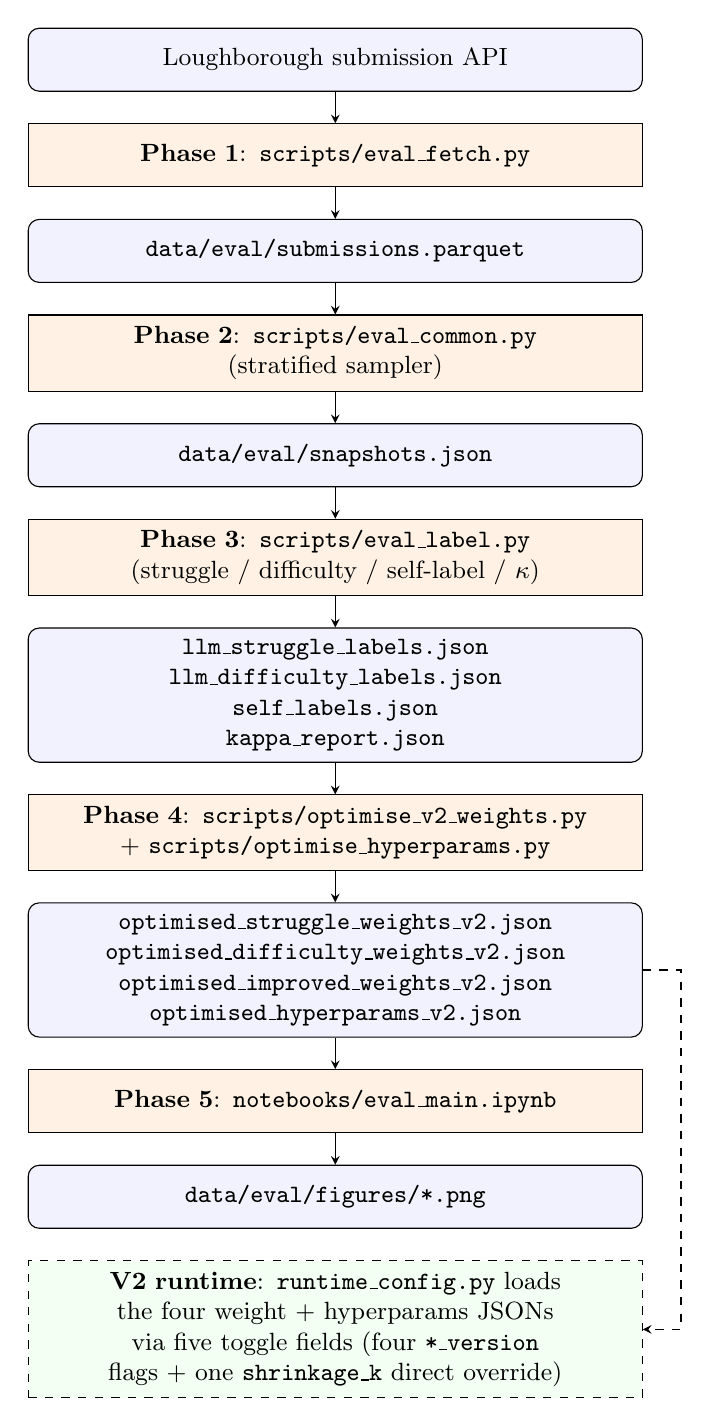
\begin{tikzpicture}[
        node distance=4mm,
        font=\small,
        artefact/.style={rectangle, draw, rounded corners, fill=blue!5,
                         text width=0.62\textwidth, align=center, minimum height=8mm,
                         inner sep=4pt},
        phase/.style={rectangle, draw, fill=orange!10,
                      text width=0.62\textwidth, align=center, minimum height=8mm,
                      inner sep=4pt},
        runtime/.style={rectangle, draw, dashed, fill=green!5,
                        text width=0.62\textwidth, align=center, minimum height=8mm,
                        inner sep=4pt},
        every path/.style={->, >=stealth}
    ]
        \node[artefact] (api) {Loughborough submission API};
        \node[phase, below=of api] (p1) {\textbf{Phase 1}: \texttt{scripts/eval\_fetch.py}};
        \node[artefact, below=of p1] (parquet) {\texttt{data/eval/submissions.parquet} };
        \node[phase, below=of parquet] (p2) {\textbf{Phase 2}: \texttt{scripts/eval\_common.py} (stratified sampler)};
        \node[artefact, below=of p2] (snapshots) {\texttt{data/eval/snapshots.json} };
        \node[phase, below=of snapshots] (p3) {\textbf{Phase 3}: \texttt{scripts/eval\_label.py} (struggle / difficulty / self-label / $\kappa$)};
        \node[artefact, below=of p3] (labels) {\texttt{llm\_struggle\_labels.json}  \\ \texttt{llm\_difficulty\_labels.json}  \\ \texttt{self\_labels.json}  \\ \texttt{kappa\_report.json}};
        \node[phase, below=of labels] (p4) {\textbf{Phase 4}: \texttt{scripts/optimise\_v2\_weights.py} + \texttt{scripts/optimise\_hyperparams.py}};
        \node[artefact, below=of p4] (weights) {\texttt{optimised\_struggle\_weights\_v2.json} \\ \texttt{optimised\_difficulty\_weights\_v2.json} \\ \texttt{optimised\_improved\_weights\_v2.json} \\ \texttt{optimised\_hyperparams\_v2.json}};
        \node[phase, below=of weights] (p5) {\textbf{Phase 5}: \texttt{notebooks/eval\_main.ipynb}};
        \node[artefact, below=of p5] (out) {\texttt{data/eval/figures/*.png} };
        \node[runtime, below=of out] (runtime) {\textbf{V2 runtime}: \texttt{runtime\_config.py} loads the four weight + hyperparams JSONs via five toggle fields (four \texttt{*\_version} flags + one \texttt{shrinkage\_k} direct override)};

        \draw (api)       -- (p1);
        \draw (p1)        -- (parquet);
        \draw (parquet)   -- (p2);
        \draw (p2)        -- (snapshots);
        \draw (snapshots) -- (p3);
        \draw (p3)        -- (labels);
        \draw (labels)    -- (p4);
        \draw (p4)        -- (weights);
        \draw (weights)   -- (p5);
        \draw (p5)        -- (out);
        \draw[dashed]     (weights.east) -- ++(0.04\textwidth,0) |- (runtime.east);
    \end{tikzpicture}
    \caption{V2 model refinement pipeline}
    \label{fig:v2-pipeline-design}
\end{figure}


\subsection{Retrieval-Augmented Generation Feedback Design}

This section describes the retrieval-augmented generation (RAG) layer that produces coaching suggestions for the lab assistants and instructors.
The architecture adopts a hybrid two-layer retrieval architecture, in which a structured pre-filter narrows the candidate set before a semantic search ranks it (Figure~\ref{fig: rag architecture}).
The design grounds LLM output in the session's own submission history; this mitigates the hallucination risk that has been flagged as a major concern when deploying generative models in educational settings \cite{lewisRetrievalAugmentedGenerationKnowledgeIntensive2020,kasneciChatGPTGoodOpportunities2023}.

\begin{figure}[H]
    \centering
    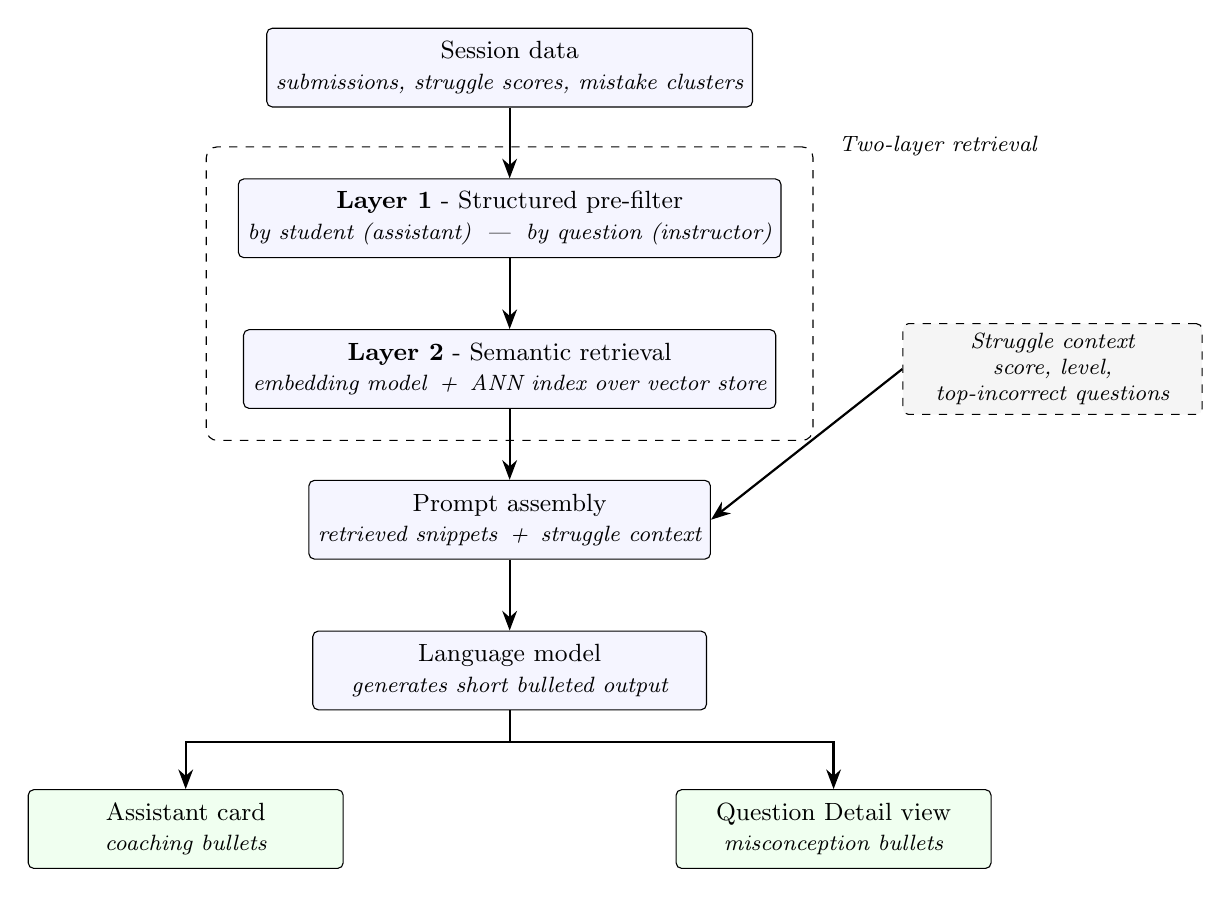
\begin{tikzpicture}[
        node distance = 0.9cm and 1.0cm,
        component/.style = {
            rectangle, draw, rounded corners=2pt,
            minimum width=5.0cm, minimum height=1.0cm,
            align=center, font=\small, fill=blue!4
        },
        sidenote/.style = {
            rectangle, draw, dashed, rounded corners=2pt,
            minimum width=3.8cm, minimum height=1.0cm,
            align=center, font=\footnotesize\itshape, fill=gray!8
        },
        output/.style = {
            rectangle, draw, rounded corners=2pt,
            minimum width=4.0cm, minimum height=1.0cm,
            align=center, font=\small, fill=green!6
        },
        flow/.style = {-{Stealth[length=2.5mm]}, thick},
        grouplabel/.style = {font=\footnotesize\itshape, anchor=west}
    ]
        % - Input -
        \node[component] (input) {Session data\\\footnotesize\itshape submissions, struggle scores, mistake clusters};

        % - Layer 1: structured pre-filter -
        \node[component, below=of input] (prefilter) {\textbf{Layer~1} - Structured pre-filter\\\footnotesize\itshape by student (assistant) \;|\; by question (instructor)};

        % - Layer 2: semantic retrieval -
        \node[component, below=of prefilter] (semantic) {\textbf{Layer~2} - Semantic retrieval\\\footnotesize\itshape embedding model \,+\, ANN index over vector store};

        % - Side-fed struggle context -
        \node[sidenote, right=1.6cm of semantic] (struggle) {Struggle context\\score, level,\\top-incorrect questions};

        % - Prompt assembly -
        \node[component, below=of semantic] (prompt) {Prompt assembly\\\footnotesize\itshape retrieved snippets \,+\, struggle context};

        % - Language model -
        \node[component, below=of prompt] (lm) {Language model\\\footnotesize\itshape generates short bulleted output};

        % - Output branches -
        \node[output, below left = 1.0cm and -0.4cm of lm] (assistant)
            {Assistant card\\\footnotesize\itshape coaching bullets};
        \node[output, below right = 1.0cm and -0.4cm of lm] (instructor)
            {Question Detail view\\\footnotesize\itshape misconception bullets};

        % - Dashed group around the two-layer retrieval -
        \begin{scope}[on background layer]
            \node[draw, dashed, rounded corners=4pt,
                  fit=(prefilter)(semantic),
                  inner sep=0.4cm] (retgroup) {};
        \end{scope}
        \node[grouplabel] at (retgroup.north east) [xshift=2mm] {Two-layer retrieval};

        % - Arrows -
        \draw[flow] (input)     -- (prefilter);
        \draw[flow] (prefilter) -- (semantic);
        \draw[flow] (semantic)  -- (prompt);
        \draw[flow] (struggle.west) -- (prompt.east);
        \draw[flow] (prompt)    -- (lm);
        \draw[flow] (lm.south)  -- ++(0,-0.4) -| (assistant.north);
        \draw[flow] (lm.south)  -- ++(0,-0.4) -| (instructor.north);
    \end{tikzpicture}
    \caption{Two-layer retrieval-augmented generation pipeline describing the whole process from session data to final output for both assistants and instructors.}
    \label{fig: rag architecture}
\end{figure}


\paragraph{Two-layer retrieval}
Each layer in the architecture applies a different selection mechanism, and the two together narrow down the search space before generation.
\begin{itemize}
    \item \textbf{Layer 1: Structured Filter -} A query about a single student is restricted to that student's submissions, and a query about a single question is restricted to submissions on that question. The pre-filter operates over the structured attributes already present in the session data, returning only the rows relevant to the query.
    \item \textbf{Layer 2: Semantic Search -} The pre-filtered submissions are ranked by similarity to the query in a vector embedding space \cite{reimersSentenceBERTSentenceEmbeddings2019}, with an approximate nearest neighbour index \cite{malkovEfficientRobustApproximate2016} used in place of exact search to keep retrieval within the dashboard's interactive refresh rate. The structured filter is repeated at this layer through metadata constraints so the two layers cannot disagree.
\end{itemize}

The pre-filter narrows the candidate set to documents that are relevant to the request; the semantic layer then ranks that smaller set by content similarity.
The reverse ordering, where the semantic search is first and the structured filter is second, would embed every submission, retrieve a globally similar subset, and then discard most of it, which wastes embedding effort on submissions that were never going to satisfy the structured constraints.

\paragraph{Prompt construction and outputs}
The retrieved documents are passed to an LLM alongside structured context derived from the rest of the dashboard: the student's struggle score and level, their highest incorrectness questions, and the retrieved submission snippets themselves. The model is instructed to return a short bulleted summary for both assistants and instructors.

\paragraph{Tailoring the pipeline to two audiences}
The same RAG pipeline serves two distinct audiences with different needs: lab assistants and instructors. 
On the assistant side, the structured pre-filter narrows to a single student and the output is framed as one-on-one coaching advice.
On the instructor side, the pre-filter narrows to a single question and the output is framed as class-wide feedback on common mistakes and misconceptions grounded in the mistake clusters from Section \ref{sec: mistake clustering}. 
Sharing the pipeline avoids duplicating the embedding and retrieval infrastructure, while the surface-specific prompts keep each output relevant to its audience.

\subsection{Interaction and UI Designs}
This section describes how the output of our models defined in Section \ref{sec: student struggle} and \ref{sec: task difficulty} is presented to instructors in a way that enables quick decision-making during lab sessions. The design is intended to provide an intuitive view.

\subsubsection{Design Principles}
The user interface is driven by the requirement to expose the model outputs defined in Sections \ref{sec: student struggle} and \ref{sec: task difficulty} in a form that enables rapid, intuitive interpretation and decision-making. Unlike the previous dashboard we explored, this one will be more intuitive and will be used primarily for computer labs.

The primary objective is to present student struggle and question difficulty as distinct signals. Student struggle indicators are derived from the struggle score $S_t(s,\sigma)$ and question difficulty indicators are derived from the difficulty score $D_t(q)$. These two indicators will prove to be valuable in helping educators improve learning outcomes.

A further objective is to allocate lab assistants to students so they can help promptly. This will send a notification to the lab assistant allocating them to students. Another is avoiding exposure of raw data, which has been mitigated by data normalisation.

Finally, the system focuses on supporting decision-making rather than explanatory analysis. The dashboard is intended to guide instructors towards timely intervention by highlighting students and tasks requiring attention and enabling efficient allocation of lab assistants.

\subsubsection{Instructor Views}
The dashboard provides a real-time overview of student struggles and question difficulty during the computer labs. The dashboard will allow the instructor to make quick decisions and aid those in need. To illustrate the proposed interface, three Figma mock-ups are presented in Figma~\ref{fig: figma1} - \ref{fig: figma3}. The deployed implementation that follows this design is described in the implementation chapter.  

\begin{figure}[H]
    \centering
    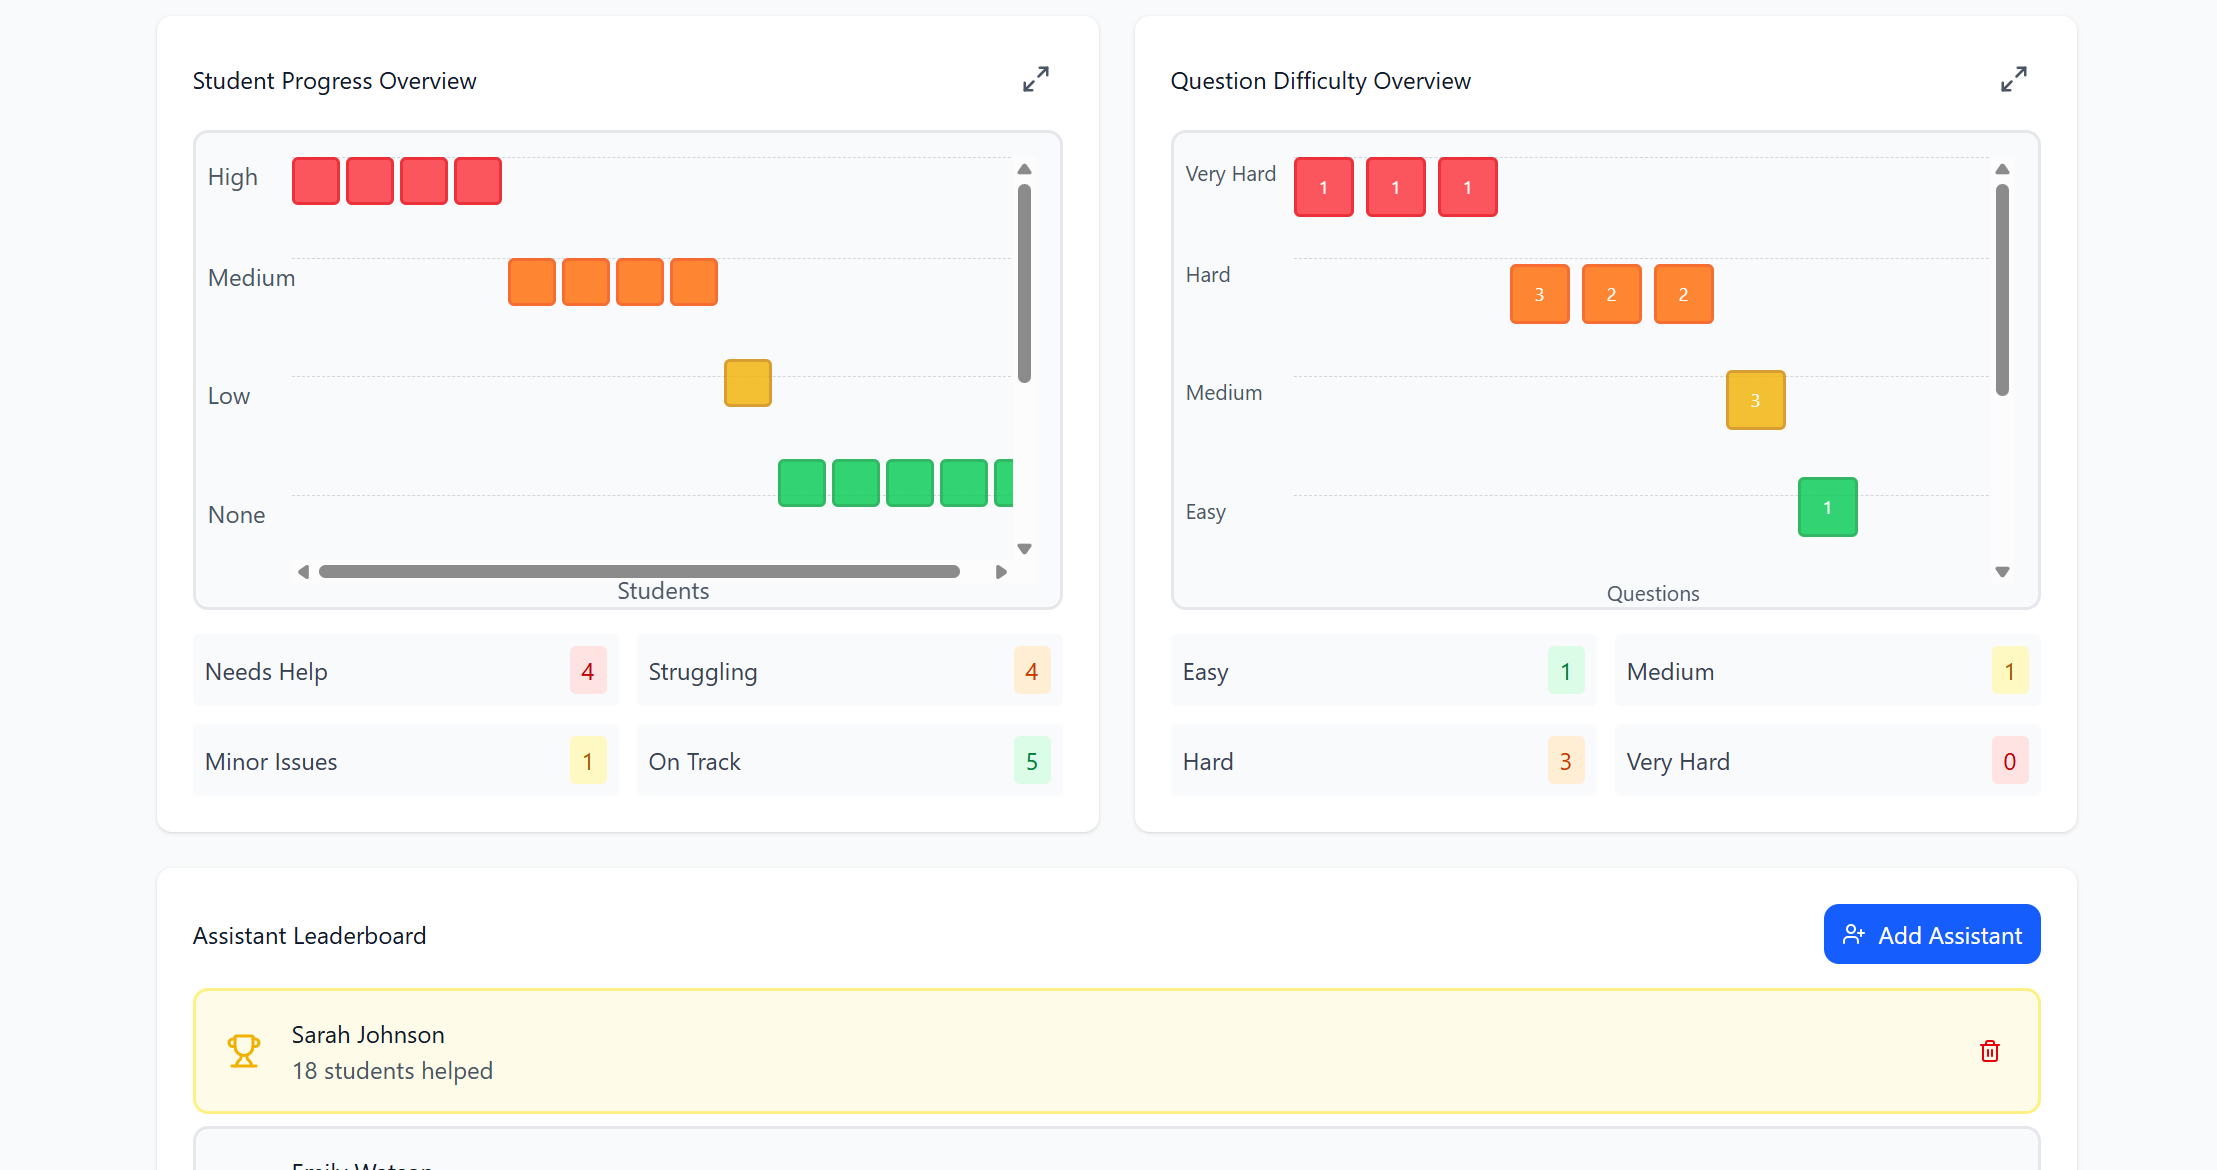
\includegraphics[width=1\linewidth]{figures/design-and-architecture/figma1.png}
    \caption{Views based on student struggle and question difficulty}
    \label{fig: figma1}
\end{figure}
As shown in Figure \ref{fig: figma1}, our dashboard has two key views: the first shows a list of students whose struggles are at certain thresholds, hence the colour; the second shows a list of questions based on difficulty at a threshold, thus the colour. The values used for comparison against the thresholds are derived from our student struggle and question difficulty equations. The view also allows instructors to go over additional information.

\begin{figure}[H]
    \centering
    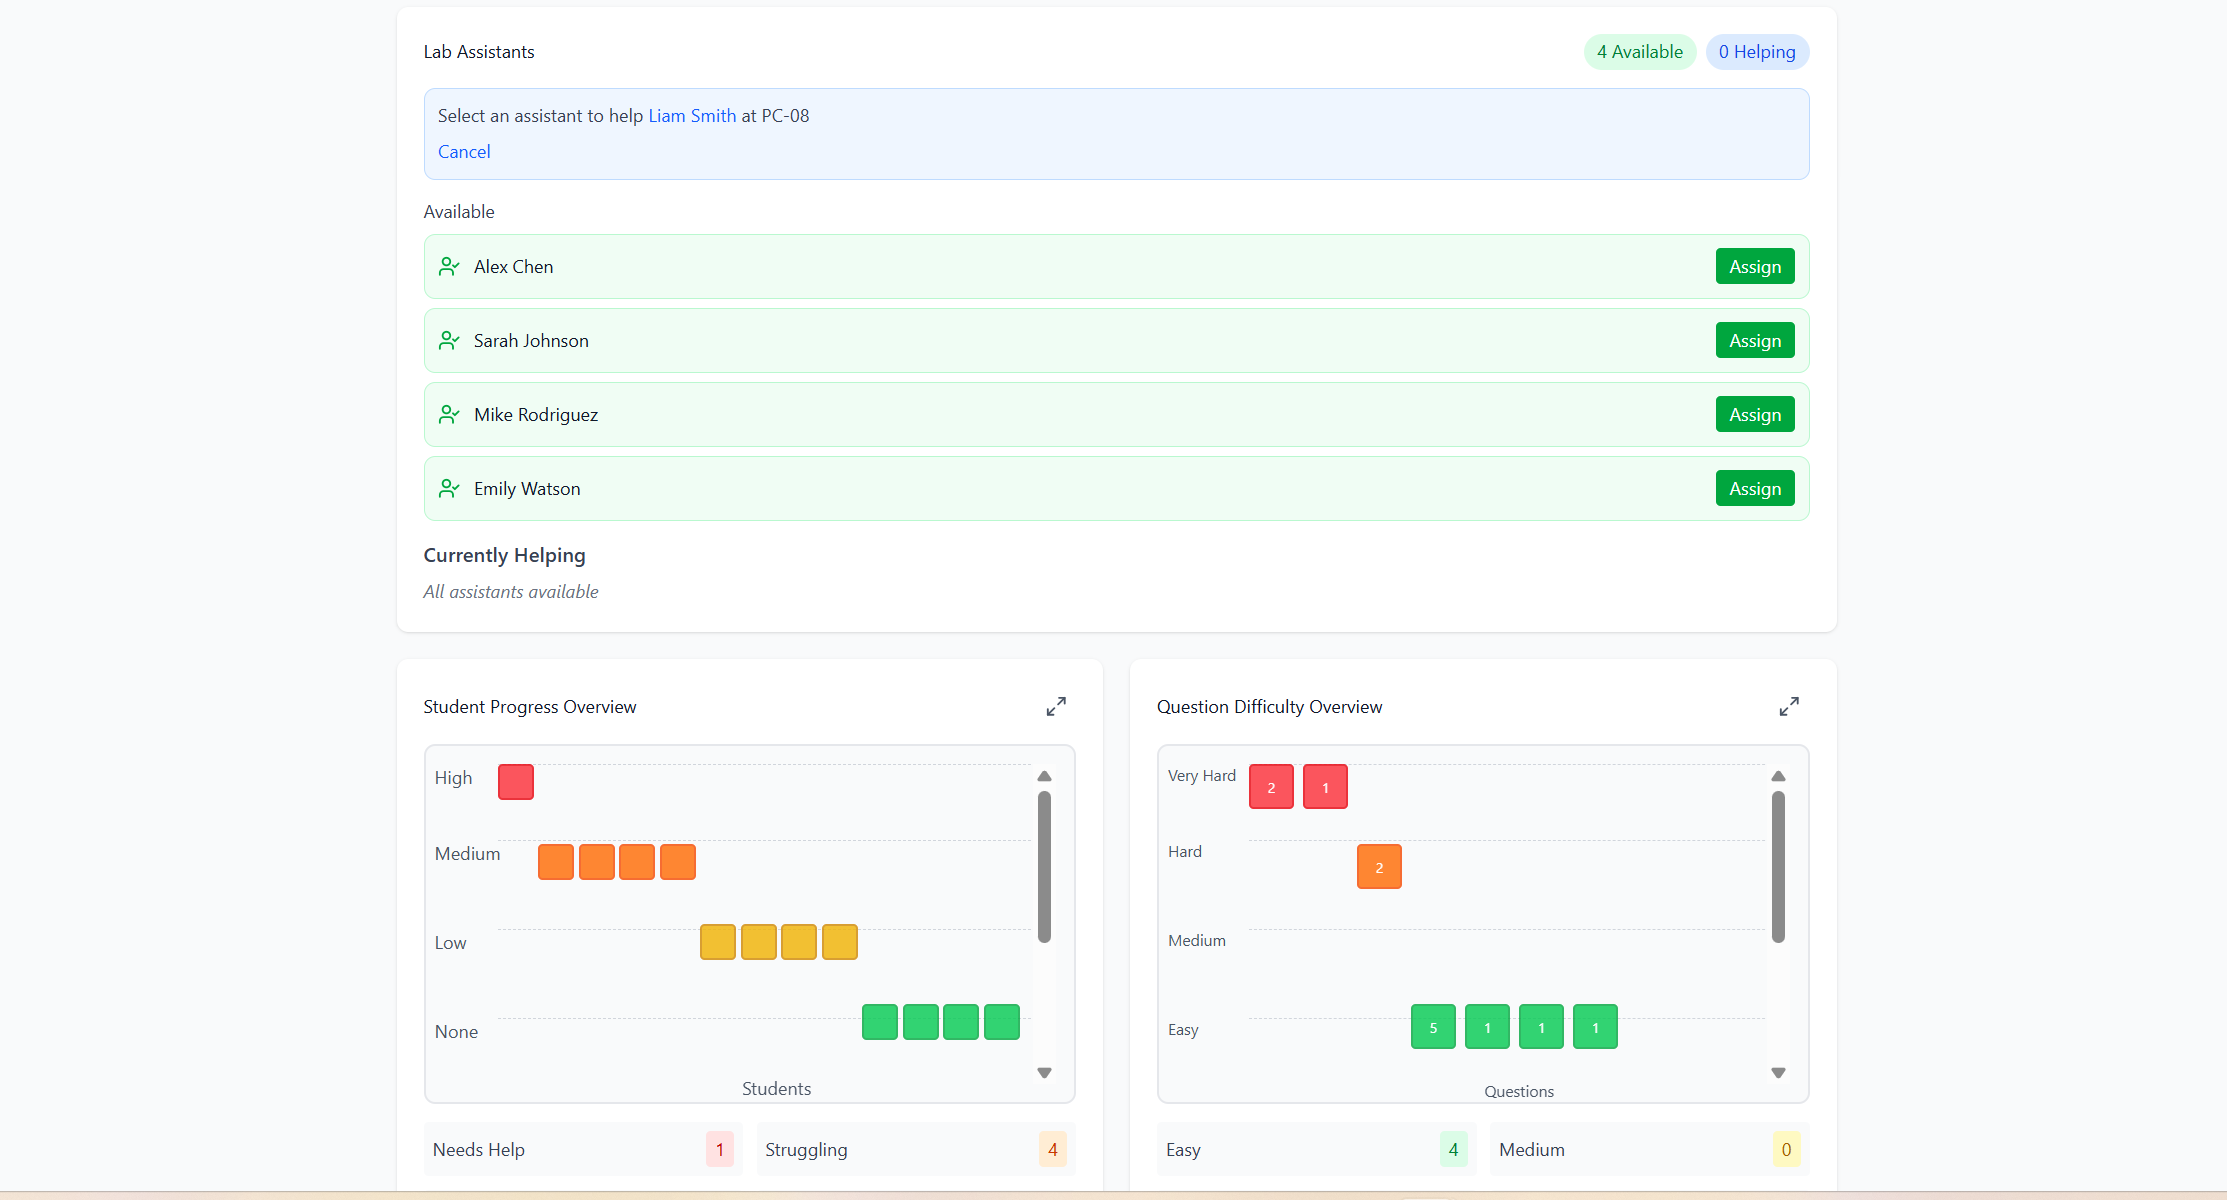
\includegraphics[width=1\linewidth]{figures/design-and-architecture/figma2.png}
    \caption{View of allocation of Lab Assistant}
    \label{fig: figma2}
\end{figure}
In Figure \ref{fig: figma2}, we can select a lab assistant and then press a student to allocate them. This is a simple approach and a very minimal, intuitive design that allows use without training on the system.


\begin{figure}[H]
    \centering
    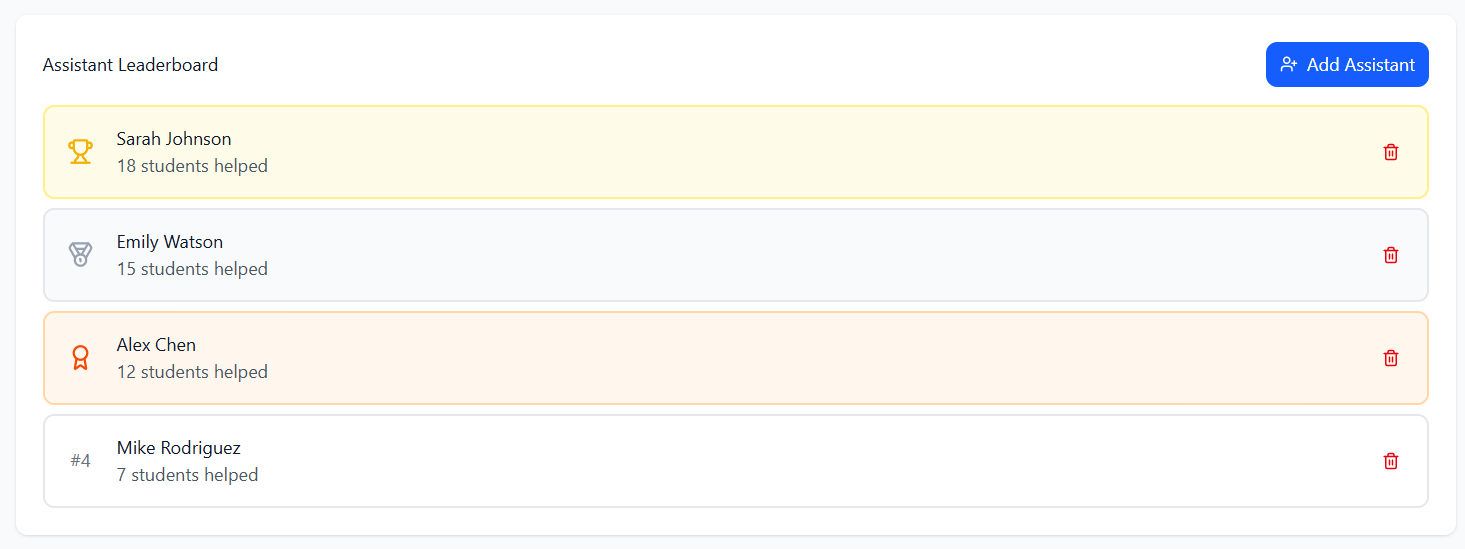
\includegraphics[width=1\linewidth]{figures/design-and-architecture/figma3.png}
    \caption{Assistant leaderboard, based on how many students have been helped}
    \label{fig: figma3}
\end{figure}
In Figure \ref{fig: figma3}, we can see that lab assistants are displayed based on their contributions. By gamifying the helping process, we can incentivise assistants to help more students.

\subsubsection{Lab Assistant View}

The lab assistant view is the mobile interface designed for assistants moving between students during a live session. Unlike the lab instructor dashboard, which assumes a stationary screen and wide canvas, the assistant view is built for short interactions on a handheld device. The interface presents one of three states at any moment, each scoped to the assistant's current responsibility: joining a session, waiting for an assignment, or helping the student they have been assigned. Figure~\ref{fig: assistant views} shows the three states in sequence.

\begin{figure}[H]
    \centering
    \begin{subfigure}[t]{0.31\linewidth}
        \centering
        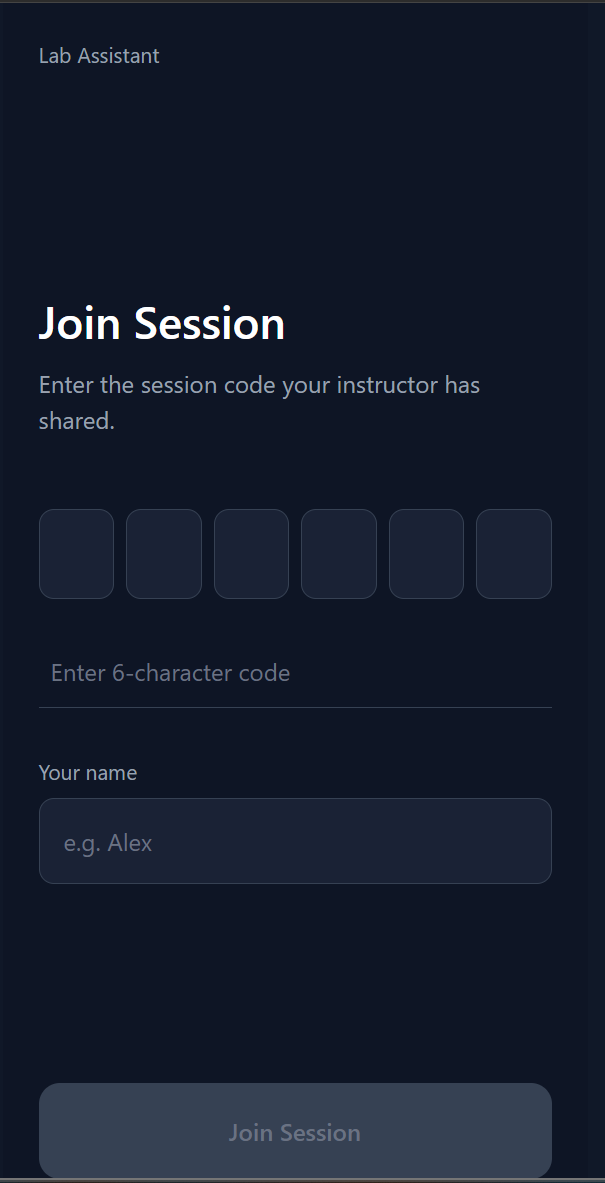
\includegraphics[width=\linewidth]{figures/design-and-architecture/figma4.png}
        \caption{Session join}
        \label{fig: figma4}
    \end{subfigure}
    \hfill
    \begin{subfigure}[t]{0.31\linewidth}
        \centering
        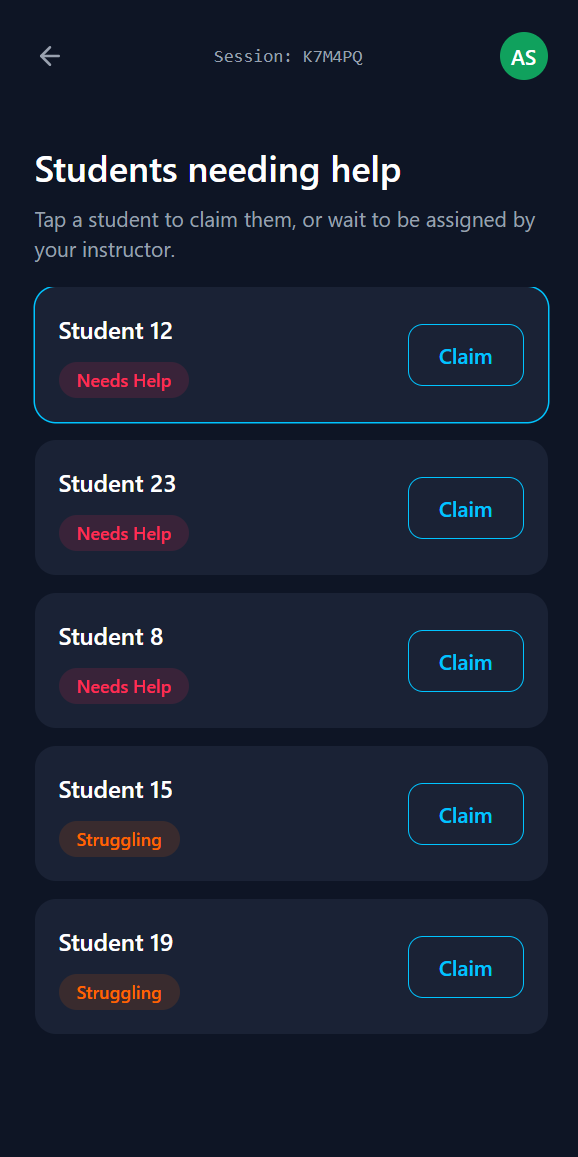
\includegraphics[width=\linewidth]{figures/design-and-architecture/figma5.png}
        \caption{Waiting for assignment}
        \label{fig: figma5}
    \end{subfigure}
    \hfill
    \begin{subfigure}[t]{0.31\linewidth}
        \centering
        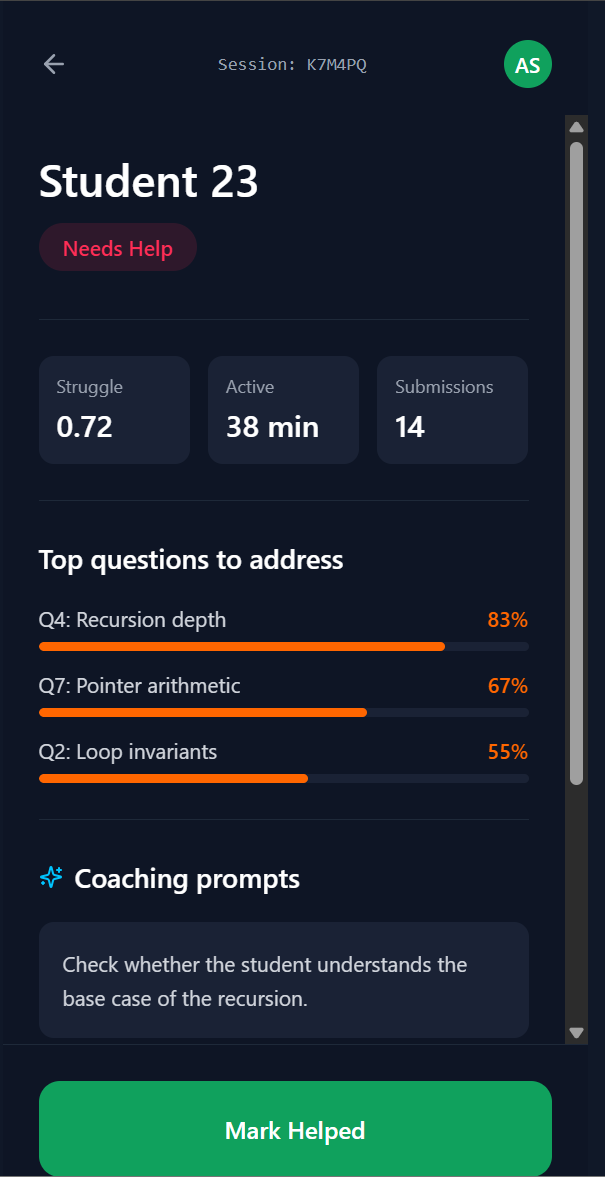
\includegraphics[width=\linewidth]{figures/design-and-architecture/figma6.png}
        \caption{Assigned student}
        \label{fig: figma6}
    \end{subfigure}
    \caption{The three states of the lab assistant view: \subref{fig: figma4} the session-join screen where the assistant enters the session code and their name; \subref{fig: figma5} the waiting state with a priority list of unassigned struggling students; \subref{fig: figma6} the assigned-student card showing struggle context, prioritised questions, and coaching prompts from the RAG layer.}
    \label{fig: assistant views}
\end{figure}

On first access (Figure~\ref{fig: figma4}), the assistant enters the session code shown on the instructor dashboard and provides their name. The session code is short enough to be read aloud by the instructor and typed without errors; the name is recorded so subsequent allocation decisions can address assistants individually. Once joined, the assistant is enrolled in the session and remains until they leave, are removed, or the session ends.

Between assignments (Figure~\ref{fig: figma5}), the assistant sees a ranked list of students currently flagged for help, ordered by their struggle score. The assistant may wait for the instructor to allocate them directly, or self-claim a student from the list when the instructor has enabled this. The same list is visible to every joined assistant; once a student is claimed, they are removed from the unassigned pool so two assistants cannot end up at the same desk.

Once a student is assigned (Figure~\ref{fig: figma6}), the view collapses to a single student card carrying the information the assistant needs at the desk: the student's current struggle context, the questions they are most incorrect on, and a short list of coaching prompts retrieved from the RAG layer described in Section~\ref{sec:rag}. A Mark Helped action lets the user know the student was helped, after which the assistant can either release the student or continue providing assistance.

\subsubsection{Visual Encoding of Metrics}

By deciding on thresholds, we can highlight a student by degree of struggle or highlight a question by degree of difficulty


\begin{table}[H]
    \centering
    \begin{tabular}{|p{0.1\textwidth}||p{0.2\textwidth}|p{0.2\textwidth}|p{0.2\textwidth}|p{0.2\textwidth}|}
    \hline
        Degree & \cellcolor{tlGreen}On Track & \cellcolor{tlAmber}Minor Issues & \cellcolor{tlOrange}Struggling & \cellcolor{tlRed}Needs Help \\
    \hline
        Threshold & $0 \leqslant S_t(s,\sigma) \leqslant t_{s1}$ & $t_{s1} < S_t(s,\sigma) \leqslant t_{s2}$&  $t_{s2} < S_t(s,\sigma) \leqslant t_{s3}$ &  $t_{s3} < S_t(s,\sigma) \leqslant 1 $\\
    \hline
    \end{tabular}
    \caption{Table Highlighting how thresholds can be indicated for struggle}
    \label{tab: struggle table}
\end{table}

\begin{table}[H]
    \centering
    \begin{tabular}{|p{0.1\textwidth}||p{0.2\textwidth}|p{0.2\textwidth}|p{0.2\textwidth}|p{0.2\textwidth}|}
    \hline
        Degree & \cellcolor{tlGreen}Easy & \cellcolor{tlAmber}Medium & \cellcolor{tlOrange}Hard & \cellcolor{tlRed}Very Hard\\
    \hline
        Threshold & $0 \leqslant D_t(q) \leqslant t_{s1}$ & $t_{s1} < D_t(q) \leqslant t_{s2}$&  $t_{s2} < D_t(q) \leqslant t_{s3}$ &  $t_{s3} < D_t(q) \leqslant 1 $\\
    \hline
    \end{tabular}
    \caption{Table Highlighting how thresholds can be indicated for difficulty}
    \label{tab: difficulty table}
\end{table}


\section{Implementation}

% TODO: write per Ch4 Rewrite Brief §4.1 — chapter intro paragraph(s) (V1/V2 framing)

\subsection{Implementation Overview}

The dashboard is deployed in two versions, both are fully featured and runnable in parallel from a single working tree. 
Version~1 (\texttt{code/}) is a Streamlit implementation that consists of two separate apps: one for instructors and one for lab assistants, each running their own Python process. 
Version~2 (\texttt{code2/}) is a single app, FastAPI process that servers both an asynchronous HTTP API at \texttt{/api/} and two buld React single-page applications (SPAs) for instructors and assistants respectively. 
V2 builds on V1, with every feature from V1 reimplemented in V2, additional features added on top and performance improvements. 
V1 is the first iteration of the dashboard, which served as a proof of concept and testbed for core features and design decisions.
V2 is the second iteration, which is a complete rewrite of V1 to address its limitations and scale up to a production-ready system. 


%A single analytical core sits behind both versions. The Python package \texttt{learning\_dashboard/} --- covering data ingestion, scoring, modelling, retrieval-augmented feedback, and saved-session persistence --- is reused by V2 unchanged, as a physical copy under \texttt{code2/learning\_dashboard/}. The only divergence between the two copies is a four-line refactor to the OpenAI-key guard that allows V2's FastAPI startup probe to verify dependencies without the application secrets present; no scoring code, no model code, and no retrieval code differs across the two versions. The two versions further share a single runtime-state file, \texttt{data/lab\_session.json}, coordinated through the \texttt{filelock} library: the live-session metadata, the joined-assistant roster, and the student-to-assistant assignment map are written and read by all three processes (V1 instructor, V1 assistant, V2 backend) under a five-second exclusive lock, so a session started in V1 becomes visible to V2 within approximately five seconds and vice versa. The implication is that the analytical contribution of this work is genuinely decoupled from the presentation layer, and the existence of V2 is itself evidence of that decoupling.

The motivation behind the second iteration of the dashboard is highlighted later on in the section. The first iteration had a Streamlit foundation that was ideal for rapid prototyping and early user feedback, but was limiting in terms of performance, scalability and flexibility. The limitation of rerunning the entire script on every interaction meant that the system struggled to maintain a responsive user experience which complicates asynchronous work. 
The second iteration addresses these limitations by moving these constraints to the presentation layer to React and the backend to FastAPI whilst keeping the analytical core untouched. 
The comparison between V1 and V2 is a recurring theme in the implementation section, as it provides a useful lens to explain the rationale behind design decisions and the trade-offs involved. 

This chapter is organised top-down so that Section \ref{sec:techstack} describes the tech stack used by both versions. 
Section \ref{sec:structure} describes the runtime processes, the shared runtime state and the deferred-actions pattern that underpins V1's reactive interactions. 
Section \ref{sec:pipeline} and \ref{sec:session} cover the data pipeline from the lab endpoint to the in-memory dataframe and the live and saved-session lifecycles. 
Section \ref{sec:analytics} covers the baseline analytics and Section \ref{sec:advanced} covers the advanced modelling layer of measurement confidence, item-response-theory difficulty, Bayesian knowledge-tracing mastery, and the improved struggle model that combines them. 
Section \ref{sec:rag} covers the retrieval-augmented feedback layer that produces real-time coaching suggestions for the lab assistant.
Section \ref{sec:views} and \ref{sec:assistant} walk through the instructor views and the lab-assistant flows respectively. 
Section \ref{sec:problems} highlights the implementation problems encountered and the resolutions adopted.


\subsection{Technology Stack} \label{sec:techstack}

% TODO: write per Ch4 Rewrite Brief §4.2 — drop in tab:techstack-v2 from Part H when ready

\subsection{System Structure} \label{sec:structure}

% TODO: write per Ch4 Rewrite Brief §4.3 — opening paragraph; reference fig:arch-v2 (architecture diagram)

\subsubsection{V1 - Instructor Process (Streamlit)} 

% TODO: write per Ch4 Rewrite Brief §4.3.1

\subsubsection{V1 - Assistant Process (Streamlit, mobile)} 
% TODO: write per Ch4 Rewrite Brief §4.3.2

\subsubsection{V2 - React + FastAPI} \label{sec:v2-react-fastapi}

% TODO: write per Ch4 Rewrite Brief §4.3.3 — open with the "Why V2?" paragraph naming concrete V1 limitations

\subsubsection{Shared Runtime State} 


% TODO: write per Ch4 Rewrite Brief §4.3.4

\subsubsection{Deferred-Actions Pattern}

% TODO: write per Ch4 Rewrite Brief §4.3.5

\subsection{Data Pipeline}

% TODO: write per Ch4 Rewrite Brief §4.4 — opening paragraph; reference fig:pipeline-flow

\subsubsection{Endpoint Retrieval and Parsing}

% TODO: write per Ch4 Rewrite Brief §4.4.1

\subsubsection{Data Normalisation and Structuring}

% TODO: write per Ch4 Rewrite Brief §4.4.2

\subsubsection{Caching Strategy}

% TODO: write per Ch4 Rewrite Brief §4.4.3

\subsection{Session Management}

% TODO: write per Ch4 Rewrite Brief §4.5

\subsubsection{Live Session Lifecycle}

% TODO: write per Ch4 Rewrite Brief §4.5.1

\subsubsection{Saved Session History and Restoration}

% TODO: write per Ch4 Rewrite Brief §4.5.2

\subsection{Analytics Implementation}

% TODO: write per Ch4 Rewrite Brief §4.6

\subsubsection{Incorrectness Scoring}

% TODO: write per Ch4 Rewrite Brief §4.6.1 — REQUIRED maths recap line (Marker-1 check)

\subsubsection{Baseline Student Struggle Model}

% TODO: write per Ch4 Rewrite Brief §4.6.2 — REQUIRED maths recap line; drop in tab:struggle-7sig

\subsubsection{Baseline Question Difficulty Model}

% TODO: write per Ch4 Rewrite Brief §4.6.3 — REQUIRED maths recap line; drop in tab:difficulty-5sig

\subsubsection{Collaborative Filtering}

% TODO: write per Ch4 Rewrite Brief §4.6.4 — REQUIRED maths recap line

\subsubsection{Mistake Clustering}

% TODO: write per Ch4 Rewrite Brief §4.6.5

\subsection{Advanced Model Implementation}

% TODO: write per Ch4 Rewrite Brief §4.7

\subsubsection{Measurement Confidence}

% TODO: write per Ch4 Rewrite Brief §4.7.1 — REQUIRED maths recap line

\subsubsection{Item Response Theory (IRT) Difficulty}

% TODO: write per Ch4 Rewrite Brief §4.7.2 — REQUIRED maths recap line; \cite{byrdLBFGSB1995}

\subsubsection{Bayesian Knowledge Tracing (BKT) Mastery}

% TODO: write per Ch4 Rewrite Brief §4.7.3 — REQUIRED maths recap line; \cite{corbettKnowledgeTracingModeling1995}; drop in tab:bkt-defaults

\subsubsection{Improved Struggle Model}

% TODO: write per Ch4 Rewrite Brief §4.7.4 — REQUIRED maths recap line

\subsection{RAG Suggested Feedback}

% TODO: write per Ch4 Rewrite Brief §4.8 — no inline supervisor attribution

\subsubsection{Hybrid Two-Layer Architecture}

% TODO: write per Ch4 Rewrite Brief §4.8.1 — include \cite{lewisRetrievalAugmentedGenerationKnowledgeIntensive2020}

\subsubsection{Embedding Model (all-MiniLM-L6-v2)}

% TODO: write per Ch4 Rewrite Brief §4.8.2

\subsubsection{Generation and Prompting}

% TODO: write per Ch4 Rewrite Brief §4.8.3

\subsubsection{Suggestion Caching}

% TODO: write per Ch4 Rewrite Brief §4.8.4

\subsubsection{Graceful Degradation and Privacy}

% TODO: write per Ch4 Rewrite Brief §4.8.5

\subsection{Instructor System Views}

% TODO: write per Ch4 Rewrite Brief §4.9.0 — opening paragraph + drop in tab:views-comparison (V1 vs V2 parity)

\subsubsection{In-Class View}

% TODO: write per Ch4 Rewrite Brief §4.9.1

\subsubsection{Student Detail View}

% TODO: write per Ch4 Rewrite Brief §4.9.2

\subsubsection{Question Detail View}

% TODO: write per Ch4 Rewrite Brief §4.9.3

\subsubsection{Data Analysis View}

% TODO: write per Ch4 Rewrite Brief §4.9.4

\subsubsection{Model Comparison View}

% TODO: write per Ch4 Rewrite Brief §4.9.5

\subsubsection{Settings View}

% TODO: write per Ch4 Rewrite Brief §4.9.6

\subsubsection{Previous Sessions View}

% TODO: write per Ch4 Rewrite Brief §4.9.7

\subsection{Lab Assistant System}

% TODO: write per Ch4 Rewrite Brief §4.10

\subsubsection{Session Join Flow}

% TODO: write per Ch4 Rewrite Brief §4.10.1

\subsubsection{Waiting and Assignment States}

% TODO: write per Ch4 Rewrite Brief §4.10.2

\subsubsection{Live Assistant Allocation and Mark-Helped}

% TODO: write per Ch4 Rewrite Brief §4.10.3

\subsection{Problems Encountered and Solutions}

% TODO: write per Ch4 Rewrite Brief §4.11 — drop in tab:problems
% Note: sound-effects discussion now lives inside §4.9.6 Settings View (the toggle is there); old standalone §4.11 Sound Effects subsection removed during 2026-05-20 layout refinement.

% Old V1-prototype draft prose has been moved to implementation-old.tex (sidecar, not \include'd in main.tex). Decision 2026-05-20: nothing in there is being reused.


\section{Evaluation} \label{sec:evaluation}

This chapter evaluates the dashboard system of Chapter~\ref{sec:implementation} along two dimensions, the validity of the model outputs (whether the struggle and difficulty rankings agree with observable student behaviour) and the operational behaviour of the deployed software against the responsiveness, interpretability, and robustness targets implied in Chapter~\ref{sec:requirements}. 
The unit of evaluation is the individual weekly lab sessions as the dashboard is designed to be used within a single session and the cohort consists of approximately 140 students. The evaluation focuses on the module from which data was collected, \textbf{25COA122}, across 23 recorded lab sessions from 2 February 2026 to 15 May 2026.
On most weeks there were two lab sessions running back-to-back, each lasting an hour, except for the first and last week which had one session each.

\subsection{Evaluation Design} \label{sec:eval-design}

\subsubsection{Scope of Evaluation}
% TODO: 5.1.1 prose block (retrospective replay choice; prospective intervention out of scope; functional verification bounded)
The evaluation is a retrospective replay of the submission logs already collected during the deployment, assessing each model output at varying cutoff points \(T\) against ground-truth labels derived from behaviour in the same logs, which lets us examine the dashboard's prioritisation as if it were running live without conducting a fresh classroom experiment.
We additionally evaluate the v2 weight vectors that were refitted against second-opinion labels obtained from an LLM rater.
A prospective intervention study, which would test whether dashboard-informed instructor decisions improve student outcomes, is explicitly out of scope; the deployment window did not permit a controlled comparison, the anonymisation of student identifiers rules out grade linkage, and submission records cannot currently be mapped to individual lab seats, so any causal interpretation is left to future work.

The functional and non-functional testing is also carried out through smoke-testing and end-to-end testing of the deployed V2 stack, where we record evidence of the system's behaviour and performance against the targets set in Chapter~\ref{sec:requirements}.
We will present a qualitative summary in the main body with the full row-by-row checklist appearing in Appendix~\ref{app:detailed-test-results}. We do not run a load test, a security audit, or an accessibility audit.

\subsubsection{Evidence Sources}
% TODO: 5.1.2 prose block

The evaluation draws on five sources of evidence. 
The primary source is the deployment submission log, a newline delimited JSON record exported from the platform's submission API and parsed by the data loader of Section~\ref{sec:analytics} into a normalised DataFrame indexed by student, question, and timestamp. 
The log spans the academic period of deployment and contains the per-submission fields the model pipeline relies on, namely the question attempted, module label, submitted answers, AI feedback and timestamp; these fields feed the derived signals recomputed at replay time.

The second source is the second-opinion label set obtained from a large language model rater (GPT-4o), which assigns each of the $1{,}306$ stratified snapshots across $140$ distinct users a struggle rating from the four defined bands, and each of the $72$ unique questions a difficulty rating from the four defined bands.
The label set is important for the training of the v2 model and its agreement against the $50$ human calibration set is reported in Section~\ref{sec:eval-compare-struggle} and also bounds the interpretive strength of the v2 numbers.

The third source is the survey of Section~\ref{sec:eval-survey}, which is an eleven-question Microsoft Forms survey distributed to undergraduate students, PhD student lab assistants and staff who are involved in computer lab sessions.
The survey provides Likert and free-text evidence on baseline lab support, dashboard interpretability, trust, and ethical concerns. 

The fourth source is the smoke testing and end-to-end testing of the deployed V2 stack, where each of the functional and non-functional requirements defined in Chapter~\ref{sec:requirements} is exercised manually and the observed behaviour recorded; the resulting checklist appears in Appendix~\ref{app:detailed-test-results}, and the body of this chapter (Section~\ref{sec:eval-functional}) records only the qualitative summary and the small number of items that failed or required workaround.

The fifth source is the V2 prewarm log, which records the wall-clock cost of each startup phase (incorrectness cache warm, IRT fit, BKT fit, struggle leaderboard, difficulty leaderboard) together with per-skill BKT predictive area under the curve (AUC) and which underpins the latency and per-skill BKT evidence reported in Section~\ref{sec:eval-results}.



\subsubsection{V2 Training Methodology} \label{sec:eval-v2-methodology}

Whilst the dashboard evaluation is primarily focused on the v1 model, a v2 model is also trained and evaluated as part of the evaluation section.
The v2 model fits the weights against second-opinion labels obtained from a large language model rater, and the resulting v2 weights are evaluated under the same evaluation framework.
Of the models introduced in Chapter~\ref{sec:implementation}, three composite weight vectors and two scalar hyperparameters are re-tuned.
The per-skill BKT parameters and the 2PL IRT parameters are retained from the fitting documented in Chapter~\ref{sec:implementation} and are not re-trained here.
The mistake-clustering pipeline, the measurement-confidence formula, and the incorrectness scorer carry no learnable weights so they are excluded from the training. 
For the evaluation we have training data which are 1{,}306 stratified snapshots across twenty-one healthy sessions for the struggle model and the improved model, and seventy-two unique questions for the difficulty model, all labelled by GPT-4o. 
The agreement between the LLM rater and a fifty-snapshot author calibration is reported in Section~\ref{sec:eval-compare-struggle}.


\subsubsection{Limitations of Evaluation}
% TODO: 5.1.4 prose block
Several limitations of the evaluation are worth noting, all of which follow from the evaluation context rather than the evaluation design. 
The first is the small effective cohort, with the v2 model training drawing on 1{,}306 stratified snapshots across twenty-one healthy sessions and 140 unique students, for the struggle model and the improved model, and 72 unique questions for the difficulty model.

The second is the single module, single institution context which limits the generalisability of the findings. 
Behaviour of the dashboard on a different module or different form of submission is not directly inferable from the results presented here, and we report findings only in the context of the 25COA122 module and the submission format of Loughborough University Computer Science lab modules. 

The third is the retrospective nature of the evaluation, which is necessary for the context of this report but still leaves a gap about whether instructor decisions actually informed by the dashboard improves student outcomes. Results focus on agreement with the LLM rater and not the causal impact on student outcomes, and any causal interpretation is left to a prospective study outside the scope of this report.


\subsection{Functional Testing} \label{sec:eval-functional}

\subsubsection{Data Ingestion and Session Handling}
The first functional requirement of Chapter~\ref{sec:requirements} (FR1, live submission-data ingestion) was validated during the V2 deployment against a live session, confirming that the JSON log returned by the Loughborough submission API is parsed correctly end-to-end into the normalised submissions DataFrame, that the XML field embedded in each record is extracted into per-submission attributes, and that the in-memory cache invalidates correctly under the configured TTL described in Section~\ref{sec:pipeline}.
Session start and end were validated through the lab instructor dashboard and the lab assistant join flow concurrently, confirming that the shared state file at \texttt{data/lab\_session.json} updates correctly under the \texttt{filelock} pattern described in Section~\ref{sec:shared-state}.
No data loss or corruption was found across the test runs. The full FR1 verification row appears in Appendix~\ref{app:detailed-test-results}.

\subsubsection{Analytics and Model Behaviour}
% TODO: 5.2.2 prose block
Functional requirements FR2 (computation of student struggle) and FR3 (computation of question difficulty) of Chapter~\ref{sec:requirements} were validated against the analytical pipeline of Chapter~\ref{sec:implementation}.
The seven-signal baseline struggle model and the five-signal baseline difficulty model were confirmed to produce scores in $[0, 1]$ across the cohort, with the four band-classification labels classifying correctly under both the v1 and v2 weight regimes.
The collaborative-filtering layer, the mistake-clustering pipeline, the IRT 2PL fit, the BKT mastery estimates, and the improved-struggle model were tested end-to-end and the outputs were cross-checked against the design equations of Chapter~\ref{sec:design}.
The graceful weight-redistribution cases described in Section~\ref{sec: improved struggle} (BKT unavailable, IRT unavailable, both unavailable) were each tested with mock data and confirmed to redistribute the weights as expected. No silent failures were observed. The per-model verification rows appear in Appendix~\ref{app:detailed-test-results}.

\subsubsection{Instructor Dashboard Features}
% TODO: 5.2.3 prose block
FR4 (real-time prioritisation) and FR5 (present relevant analytics) of Chapter~\ref{sec:requirements} were validated through the V2 FastAPI + React stack.
Each of the seven instructor views was exercised to confirm the rendered components matched the design specification: the In-Class leaderboards are ordered by score under both the Basic and Advanced modes, the band colour coding tracks the threshold classification map of Section~\ref{sec: student struggle}, and the Student Detail, Question Detail, Data Analysis, Session Progression, Previous Sessions, and Settings views render without errors.
Navigation between views was tested and confirmed to be smooth and error-free, and the data displayed in each view was cross-checked against the expected output from the analytics pipeline.
The filtering of the system was also tested to confirm that the per-module and per-session filters correctly update the displayed data and that the system handles edge cases gracefully.
Screenshots for each view appear in Appendix~\ref{app:ui-screenshots}; the full FR4 and FR5 verification rows are in Appendix~\ref{app:detailed-test-results}.

\subsubsection{Lab Assistant Workflow}
% TODO: 5.2.4 prose block
FR7 (lab assistant ranking system) of Chapter~\ref{sec:requirements} was validated through the V2 lab-assistant single-page application.
The join flow was tested with the six-character session code described in Section~\ref{sec:assistant}, confirming that the assistant's identity persists across reloads through the \texttt{?aid=} URL parameter and that the polling cycle picks up new assignments without manual refresh.
The mark-helped round-trip was validated, confirming that a button press on the assistant app updates \texttt{data/lab\_session.json} through the same file-locked pattern as the instructor process and that the instructor dashboard sidebar picks up new assistants and their status correctly.
Assistants were also confirmed to be able to join simultaneously without loss of data.
FR6 (smart device) was scoped out at design time due to focusing on the modelling; it remains future work and is restated in Section~\ref{sec:eval-discussion}. The full FR7 verification row appears in Appendix~\ref{app:detailed-test-results}.


\subsection{Non-Functional Testing} \label{sec:eval-nonfunctional}

\subsubsection{Performance and Refresh Behaviour}
NFR1 (Real Time Performance) of Chapter~\ref{sec:requirements} is met through a lifespan prewarm strategy of Chapter~\ref{sec:implementation}, which pre-computes all derived signals before the FastAPI process accepts requests so taht the first user request sees the steady state latency of the dashboard rather than the startup latency. 
The prewarm is made up of six stages, captured across a representative session of $42{,}443$ submission records across $3{,}935$ unique feedback strings.

The submission log loads and parses in $8.0$~s. The OpenAI incorrectness scoring pass runs in $464.5$~s on a cold start with an empty cache, batching $197$ calls for the $3{,}935$ unique feedback strings, but reduces to a sub-second lookup on subsequent runs through the disk-persisted cache at \texttt{data/incorrectness\_cache.json}; this $71\%$ cold start cold only occurs once pre corpus and never appears in the steady state afterwards. 
The BKT parameter fit across the six skills present in the cohort runs in $23.2$~s, fitting three skills and falling back to \texttt{config.py} defaults on three under the gating logic of Section~\ref{sec: bkt}. 
The IRT 2PL fit completes in $7.3$~s on the final $127 \times 86$ response matrix produced by the iterative min-attempts and separable-response drop-pass of Section~\ref{sec: irt}. 
The struggle leaderboard becomes ready $6.2$~s after the IRT fit and the difficulty leaderboard $3.6$~s after that. The RAG collection takes $137.2$~s to load the sentence-transformers \texttt{all-MiniLM-L6-v2} model and embed $3{,}069$ sampled rows into the in-memory vector index.

Total prewarm for this session is $649.9$~s on the cold start and approximately $185$~s on a warm start once the incorrectness cache is populated; the RAG embdeding is the largest contributor to the prewarm time. 
Once the prewarm completes, all subsequent requests respond from in-memory state and the steady-state five-second polling cycle of the lab-assistant app was confirmed to be responsive without observable latency on the observed session.  
The full NFR1 verification row appears in Appendix~\ref{app:detailed-test-results}.

\subsubsection{Usability and Interpretability}
% TODO: 5.3.2 prose block

NFR2 (Interpretability) of Chapter~\ref{sec:requirements} is supported through the design of the instructor dashboard and the survey of Section~\ref{sec:eval-survey}, which evaluated the clarity of the underlying struggle and difficulty scores as well as the intuitiveness of the colour-coded band labels surfaced in the leaderboards. 
On the five-point clarity scale of what each metric means (Q5 of the survey), seven of the ten respondents rated both the struggle and difficulty scores as "Completely Intuitive" and a further two rated them as "Slightly Intuitive"; the same single respondent placed both metrics in the "Slightly Unintuitive" band and no respondent picked either "Neutral" or "Completely Unintuitive" on either metric, yielding a strongly bimodal distribution where disagreement collapses to a single outlier.
On the five-point intuitiveness scale for the colour-coded bands (Q6), the same bimodal pattern held with six respondents at "Completely Intuitive" and three at "Slightly Intuitive" on both band sub-rows, with the same outlier at "Slightly Unintuitive".
The trust question (Q7) returned two respondents at "Very Likely" and five at "Somewhat Likely" to trust the dashboard's prioritisation, one respondent at "Neither Likely nor Unlikely", and two participants on the negative end of the scale (one at "Somewhat Unlikely" and one at "Very Unlikely"); this yielded a $70/10/20$ split between positive, neutral, and negative trust.
The question on what the main issue is when providing real-time support (Q4) had three main themes: not enough staff, quieter students may not be willing to ask for help and identifying who needs the most help is difficult which the dashboard targets. 
NFR2 is met for the surveyed cohort within the limitations of the sample size; the full NFR2 verification row appears in Appendix~\ref{app:detailed-test-results}.

\subsubsection{Robustness and Failure Handling}
% TODO: 5.3.3 prose block

\subsection{Results} \label{sec:eval-results}

\subsubsection{Baseline System Outputs}
% TODO: 5.4.1 prose block

\subsubsection{Inter-rater Agreement (Cohen's $\kappa$)} \label{sec:eval-compare-struggle}
% TODO: 5.4.2 prose block (~150 words, 3 κ statistics + Landis-Koch interpretation + within-1-band agreement; rater calibration before findings; see drafting plan Insertion 3c)

\subsubsection{Model Comparison} \label{sec:eval-compare-difficulty}
% TODO: 5.4.3 prose block (~400 words; baseline vs improved for BOTH composites: Spearman ρ + top-10 overlap + level agreement + largest movers for struggle, then same four for difficulty + 2PL discrimination diagnostic; see drafting plan §5.4.3 merged block — needs new draft)

\subsubsection{Per-Module Normalisation Effect}
% TODO: 5.4.4 prose block (was 5.4.5 pre-trim; fig:eval-permodule-normalisation, fig:eval-violin-permodule-difficulty)

\subsubsection{Hyperparameter optimisation} \label{sec:eval-hyperopt}
% TODO: 5.4.5 prose block (was 5.4.9 pre-trim; ~290 words, Optuna TPE with Spearman ρ objective for K and τ; K tied within noise (Δρ +0.013); τ substantial Δρ +0.200; joint K×τ study confirms independence; figures fig:eval-hyperparams-contour + fig:eval-hyperparams-importances + table tab:eval-hyperparams; see drafting plan §5.4.9 block)

\subsubsection{Findings} \label{sec:eval-findings}
% TODO: 5.4.6 prose block (was 5.4.10 pre-trim; ~900 words; all three v2 weight-refit findings as one continuous narrative: positive struggle v1↔v2 (ρ +0.588) + moderate-positive difficulty (ρ +0.468) + weaker-positive improved-struggle (ρ +0.201 at RF ceiling) + 4-positive-1-tie verdict scorecard; figures fig:eval-weights-struggle, fig:eval-rho-perfold-struggle, fig:eval-ols-diagnostic (supplementary), fig:eval-negative-findings + tables tab:eval-weights-struggle, tab:eval-weights-difficulty, tab:eval-weights-improved, tab:eval-verdict-scorecard; see drafting plan §5.4.10 block)


\subsection{Survey} \label{sec:eval-survey}

\subsubsection{Instrument, Audience and Ethical Approval}
% TODO: 5.5.1 prose block (11 questions; Microsoft Forms; n=8 at 2026-05-24, target ~10; tab:eval-survey-summary)

\subsubsection{Baseline Perception of Lab Support}
% TODO: 5.5.2 prose block (Q2 + Q3 + Q4 themes; fig:eval-survey-baseline)

\subsubsection{Dashboard Interpretability and Trust}
% TODO: 5.5.3 prose block (Q5 + Q6 + Q7; fig:eval-survey-clarity, fig:eval-survey-trust)

\subsubsection{Student Comfort and Ethical Concerns}
% TODO: 5.5.4 prose block (Q8 + Q9 + Q10; fig:eval-survey-comfort, fig:eval-survey-themes)

\subsubsection{Change Requests and Triangulation with Quantitative Results}
% TODO: 5.5.5 prose block (Q11; triangulation with 5.4 findings)

\subsection{Discussion} \label{sec:eval-discussion}

\subsubsection{Model Disagreement}
% TODO: 5.6.1 prose block

\subsubsection{Tradeoffs and Threats to Validity}
% TODO: 5.6.2 prose block

\subsubsection{Limitations}
% TODO: 5.6.3 prose block


% \section{Progress Report}

\subsection{Progress Status Overview}
For the January milestone, the project is progressing smoothly.
The Literature Review and Design Sections have been completed.
A working Version 1 prototype has been implemented. 
Student Struggle and Question Difficulty models have been developed
\subsection{Work Completed to Date}
The following work has been completed as part of the project:
\begin{itemize}
    \item A relevant literature review covering learning analytics, real-time dashboard and existing education systems
    \item Formulation of functional and non-functional system requirements
    \item Design of overall system architecture, including the data flow and component interactions
    \item Definitions of mathematical models for student struggle and question difficulty
    \item Implementation of Version 1 data pipeline using refreshing and session-level aggregation
    \item Development of a working instructor-facing dashboard prototype using Streamlit    
\end{itemize}
This work establishes a solid foundation for future work.

\subsection{Current Limitations}
The version 1 dashboard comes with a range of limitations:
\begin{itemize}
    \item Struggle is currently based on a single metric as a proof of concept
    \item AI Based classifications and question difficulty have not been implemented
    \item Data ingestion relies on refreshing rather than an event-driven architecture
    \item No task allocaiton to lab assistants
\end{itemize}

\subsection{Planned work}
The remaining work will focus on:
\begin{itemize}
    \item integrating the proposed analytics into the existing pipeline 
    \item replacing refresh ingestion logic with an event-driven logic.
    \item survey from both students and teachers
    \item Task allocation to lab assistants through smart devices
\end{itemize}

\subsection{Gantt Chart}

\begin{figure}[H]
    \centering
    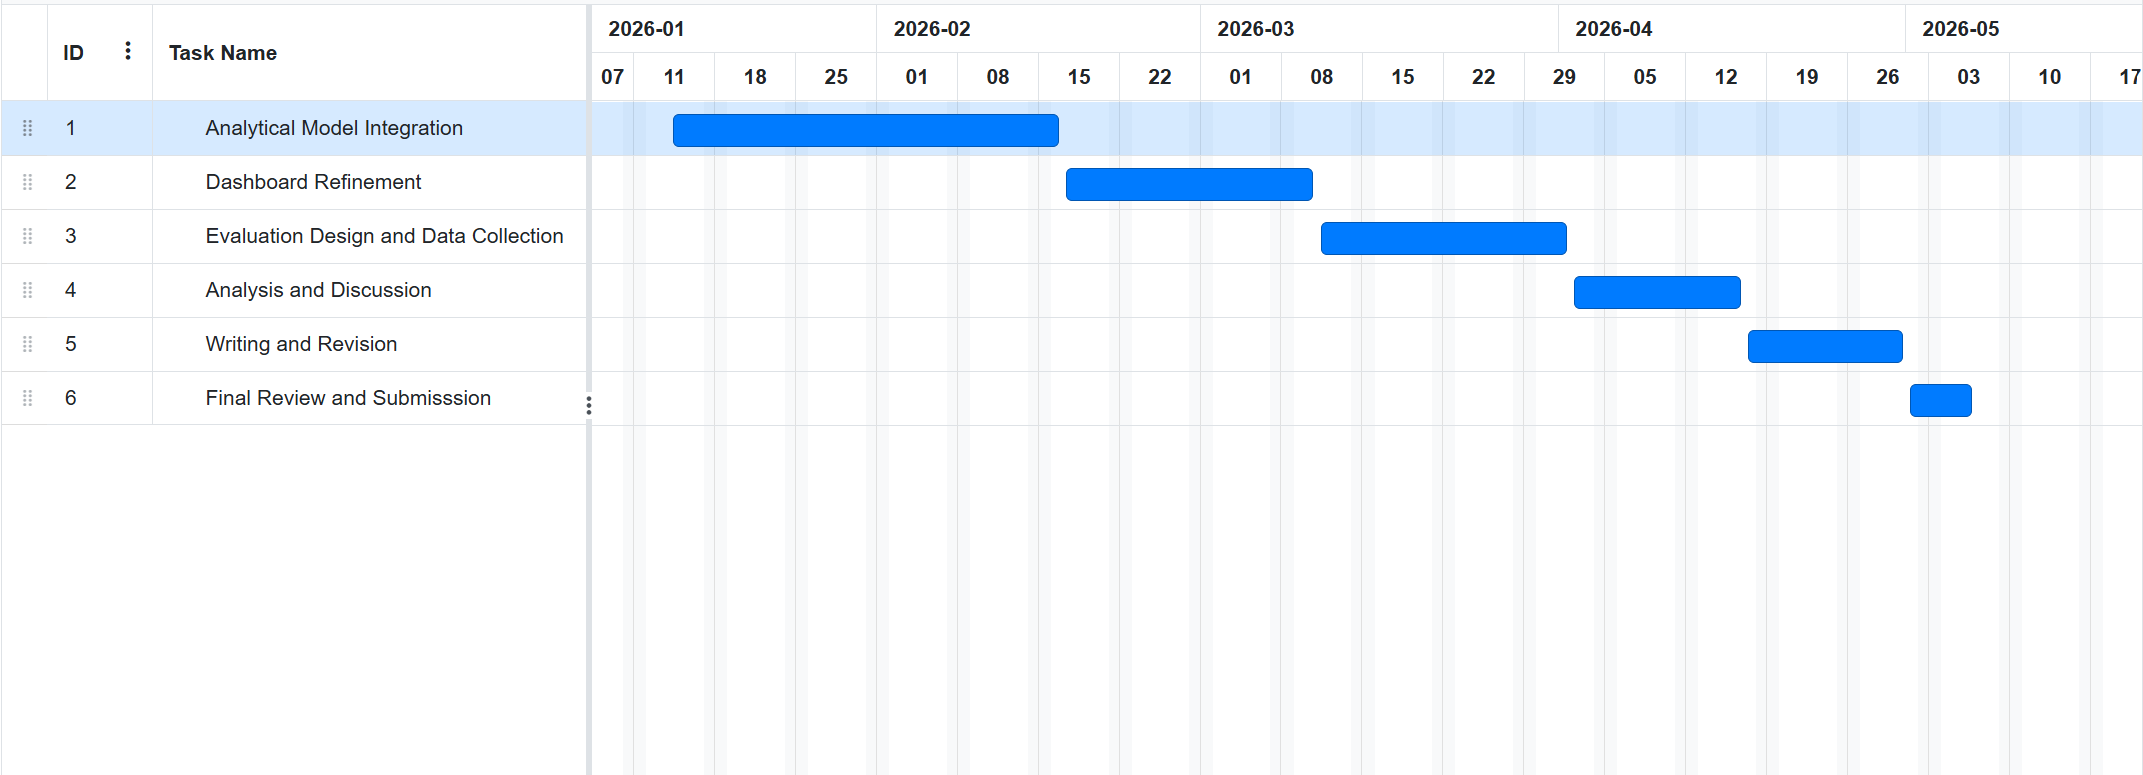
\includegraphics[width=1.2\textwidth]{figures/gantt.png}
    \caption{Project timeline from January 2026 to final submission in May 2026}
    \label{fig: Gantt}
\end{figure}


\begin{table}[H]
    \centering
    \begin{tabular}{|p{0.3\textwidth}|p{0.3\textwidth}|p{0.3\textwidth}|}
    \hline
       Task  & Start Date & End Date \\
    \hline
    \hline
       Analytical Model Integration  & 14/1/26 & 16/2/26\\
    \hline
        Dashboard Refinement & 17/2/26 & 10/3/26\\
    \hline
        Evaluation Design and Data Collection & 11/3/26 & 1/4/26\\
    \hline
        Analysis and Discussion& 2/4/26 & 16/4/26\\
    \hline
         Writing and Revision& 17/4/26 & 30/4/26\\
    \hline
         Final Review and Submission & 1/5/26 & 6/5/26\\
    \hline

    \end{tabular}
    \caption{Summary table for what is in the Gantt Chart}
    \label{tab: gantt summary}
\end{table}

\section{Conclusion} \label{sec:conclusion}

\subsection{Summary of the Project}

This project addressed a recurring practical problem in university computer labs: instructors and lab assistants cannot reliably see, in real time, which students are struggling and which questions are causing the most difficulty across a session of several dozen to over a hundred concurrent learners.
The resolution is a React and FastAPI dashboard, V2 in the staged Streamlit-then-React evolution recorded in Chapter~\ref{sec:implementation}, that ingests live submission data, computes interpretable struggle and difficulty scores from that data, and surfaces both as ranked leaderboards alongside a mistake-cluster view, a collaborative-filtering recommender, a saved-session archive, Item Response Theory and Bayesian Knowledge Tracing layers for advanced modelling, and a Retrieval-Augmented Generation feedback panel.
A second route on the same FastAPI process hosts the mobile lab-assistant interface, so coordination between the instructor and the floor team runs through a single shared session state.

The seven objectives stated in Section~\ref{sec: intro} were addressed in order.
The literature review in Chapter~\ref{sec:requirements} identified the dashboard space and surfaced the gaps in real-time, lab-scale, instructor-facing analytics; the same chapter formalised the functional and non-functional requirements that drove the rest of the project.
Chapter~\ref{sec:design} set out the data model that turns raw submission attempts into the per-student and per-question signals the scorers consume, and it defined the system architecture - shared-state coordination, view routing, caching - that Chapter~\ref{sec:implementation} then implemented.
The struggle and difficulty composites were specified in Chapter~\ref{sec:design} and refit against second-opinion labels from a large language model rater in Section~\ref{sec:eval-results}, covering composite weights, scalar hyperparameters, and band thresholds.
The dashboard itself was built incrementally from the V1 Streamlit reference to the V2 React and FastAPI implementation documented in Chapter~\ref{sec:implementation}.
Functional and non-functional evaluation followed in Chapter~\ref{sec:evaluation}, combining a retrospective replay of the deployment cohort with an eleven-question instructor and student survey.

Against the rater's four-band rating, the deployed composite achieved Spearman $\rho = +0.588$ on the struggle target and $\rho = +0.468$ on difficulty (Section~\ref{sec:eval-results}); after a constrained cross-validated brute-force search the deployed cutpoints lifted linear-weighted Cohen's $\kappa$ to $+0.384$ for struggle and $+0.387$ for difficulty (Section~\ref{sec:eval-thresholds}).
The 2PL Item Response Theory difficulty model was retained as a complementary toggle but not promoted to be the deployed scorer: its band agreement against the rater was marginally negative ($\kappa = -0.024$ at trained thresholds) and the top-ten hardest set overlapped with the composite's by one question in ten (Section~\ref{sec:eval-irt}).
The system is deployed and in use; the sections that follow set out what the validation contributed and what remains for future work.

\subsection{Key Findings and Contributions}

The first contribution is a systematic empirical validation of every tunable component of the deployed scoring pipeline against second-opinion labels from a large language model rater, with positive and negative findings reported in equal weight.
The validation covered three tiers of parameter.
The composite weights were refit by ordinary least-squares regression against the four-band rater target (Section~\ref{sec:eval-results}); the two scalar hyperparameters, the Bayesian shrinkage constant $K$ and the collaborative-filtering threshold $\tau$, were tuned by Tree-structured Parzen Estimator across fifty-trial Optuna studies (Section~\ref{sec:eval-hyperopt}); and the score-to-band thresholds were trained by brute-force linear-weighted $\kappa$ maximisation across six model variants under constrained group five-fold and leave-one-out cross-validation (Section~\ref{sec:eval-thresholds}).

The positive findings are concrete.
Tuning $\tau$ from the hand-set $0.7$ to the tuned $0.900$ raised Spearman $\rho$ by $+0.160$, a substantial gain indicating the initial setting was too permissive.
Four of the six threshold variants cleared the pre-registered promotion bar of $\Delta\kappa \geq +0.05$ under constrained cross-validation, and a follow-up search on the deployed min-max composite produced the cutpoints now in \texttt{config.py} with band-agreement $\kappa = +0.384$ for struggle and $\kappa = +0.387$ for difficulty.
The negative findings are reported with the same emphasis.
The shrinkage constant $K$ moved from the hand-set $5$ to the tuned $0$ but the gain $\Delta\rho = +0.009$ sat within per-fold standard deviation, validating the hand-set value rather than refining it.
The 2PL IRT difficulty model failed to clear the band-agreement bar at any threshold pass, with $\kappa = -0.016$ at hand-set cutpoints and $\kappa = -0.024$ at trained cutpoints, and was retained as a complementary view rather than promoted to the deployed scorer (Section~\ref{sec:eval-irt}).
The contribution is the systematic coverage and the documented negative findings.

The second contribution is the training methodology itself, reusable beyond this dashboard.
The methodology has three components.
The supervision target is a four-band ordinal rating (On Track / Minor Issues / Struggling / Needs Help on struggle; Easy / Medium / Hard / Very Hard on difficulty) produced by a large language model rater shown per-snapshot and per-question signals.
The estimator is ordinary least-squares over the composite features rather than gradient boosting or random forest.
The evaluation metric stack is Spearman $\rho$ for ranking, linear-weighted Cohen's $\kappa$ for band agreement, and mean absolute error for calibration, replacing the binary-only AUC of the original framing.

The model-class-selection rigour is the bake-off in Section~\ref{sec:eval-results}: ordinary least-squares regression was benchmarked against random forest and gradient boosting across all three targets under matched cross-validation.
Ordinary least-squares won the struggle target decisively at $\rho = +0.588$ against the next-best random forest at $\rho = +0.565$, tied the difficulty target within per-fold noise at $\rho = +0.468$ against random forest's $\rho = +0.479$, and was the only competitive class with interpretable signed weights.
Tree based alternatives offered no consistent gain large enough to outweigh that interpretability and were dropped from the deployed path.


\subsection{Future Work}

\paragraph{Cross-session aggregation}
The deployed dashboard reports struggle and difficulty within a single live session.
A respondent to the closing survey question (Section~\ref{sec:eval-survey}, Q11) asked for a view of how frequently a given student is flagged as struggling across multiple lab sessions, not just within one.
Implementing this requires persisting per-snapshot scoring beyond the live session window and aggregating per-student across sessions in a way that respects the session-grouped cross-validation structure used in evaluation.
This is the most direct survey-driven feature request in the chapter.

\paragraph{Joint weight and threshold optimisation via ordinal logistic regression}
The pipeline currently trains composite weights (Section~\ref{sec:eval-results}) and band thresholds (Section~\ref{sec:eval-thresholds}) in two separate passes; the recalibration pass on the deployed min-max composite was needed because the originally-promoted cutpoints were fit against a different score scale than the one the deployed system serves.
A proportional-odds ordinal logistic regression, fit either through \texttt{mord} or \texttt{statsmodels.OrderedModel}, would optimise the weights and the cutpoints jointly against the four-band ordinal target in a single fit, removing the scale-mismatch failure mode at its root rather than recalibrating around it.

\paragraph{Cohort-balanced re-evaluation}
The validation cohort produced no questions in the rater's "Easy" band and only $5.8\%$ of snapshots in the "On Track" band; the cohort distributions reported in Section~\ref{sec:eval-results} reflect a cohort skewed toward higher difficulty and lower performance which may be due to no intervention.
The lowest band of each scorer is therefore effectively empty on this cohort, so band-agreement findings against the rater are conditioned on a distribution the next cohort may not replicate.
Re-running the evaluation on a more balanced cohort, or on stratified sub-cohorts of the same module, would test whether the recalibrated cutpoints generalise and whether the IRT difficulty anti-result holds on a less-skewed response matrix.

\paragraph{Per-semester threshold re-tuning as a maintenance concern}
Following directly from the cohort caveat in Section~\ref{sec:eval-thresholds}, the threshold-training pass should be re-run per module rather than the existing tuples reused indefinitely.
This is a deployment-side machine-learning maintenance concern rather than a model-design change: the underlying composite score and threshold is not portable across cohorts, and the maintenance loop should recognise that.

\paragraph{Restoring the OpenAI incorrectness scorer to a non-fallback rate}
Section~\ref{sec:eval-tradeoffs} flags this as the highest-leverage future change in the evaluation chapter, ranking above retraining any of the weights or thresholds.
The OpenAI incorrectness scorer fell back to a midpoint score on $92.5\%$ of the production submissions, which propagates into the composite as noise on the strongest single signal in the weight vector.
A more robust scorer path: retry logic with backoff, structured-output validation, or a local fallback model rather than a midpoint imputation would raise the ceiling on every downstream model in the pipeline.

\paragraph{Prospective intervention study}
The retrospective replay design used in Chapter~\ref{sec:evaluation} explicitly scopes out a prospective intervention study, in which dashboard-informed instructor decisions are compared with a control group on student outcomes.
A future evaluation pass would need a controlled comparison, a lift of the student-identifier anonymisation that currently rules out grade linkage, and a submission-to-lab-seat mapping that does not exist in the current data path.
This is named here as the next-generation evaluation step rather than as an immediate follow-up; it is the only way to attribute outcome changes to the dashboard rather than to correlations with it.

\paragraph{Smart device integration}
The original scope in Section~\ref{sec: intro} named smartwatch and smart-glasses notifications to lab assistants as a secondary aim.
The V2 deployment scoped this down to a mobile lab-assistant web route served by the same FastAPI process, which delivers the same coordination affordance through a web interface rather than a native device.
Future work would restore the original goal with native notifications to a wearable, layered over the same file-locked shared-state coordination V2 already uses for cross-stack session synchronisation.
This closes the loop on the secondary aim from Chapter~\ref{sec: intro} rather than the modelling-side findings that drive the earlier items.

\appendix

% \section{Code Snippets}
\label{app:code}

This appendix shows the principal analytical functions of the deployed system together with the offline pipeline used to train and validate it. Every listing is included from its source file at the stated line range, so the code shown here is exactly the code that runs. The analytical core of V2 is organised as per-concern modules under \texttt{code2/backend/}, and the evaluation and training scripts live under \texttt{scripts/}.

% Source files are UTF-8; listingsutf8 reads them without splitting multi-byte
% sequences, and the literate map below lets pdflatex render the Greek/maths
% glyphs that appear in code comments. Scoped to this appendix (Ch4 listings are
% already typeset by the time this \lstset runs).
\lstset{
  inputencoding=utf8/latin1,
  extendedchars=true,
  columns=fullflexible,
  basicstyle=\scriptsize\ttfamily,
  literate=%
    {α}{{$\alpha$}}1 {β}{{$\beta$}}1 {γ}{{$\gamma$}}1 {δ}{{$\delta$}}1
    {ε}{{$\epsilon$}}1 {ζ}{{$\zeta$}}1 {η}{{$\eta$}}1 {θ}{{$\theta$}}1
    {ι}{{$\iota$}}1 {κ}{{$\kappa$}}1 {λ}{{$\lambda$}}1 {μ}{{$\mu$}}1
    {ν}{{$\nu$}}1 {ξ}{{$\xi$}}1 {π}{{$\pi$}}1 {ρ}{{$\rho$}}1
    {σ}{{$\sigma$}}1 {τ}{{$\tau$}}1 {φ}{{$\phi$}}1 {χ}{{$\chi$}}1
    {ψ}{{$\psi$}}1 {ω}{{$\omega$}}1
    {Δ}{{$\Delta$}}1 {Σ}{{$\Sigma$}}1 {Π}{{$\Pi$}}1 {Ω}{{$\Omega$}}1
    {Θ}{{$\Theta$}}1 {Λ}{{$\Lambda$}}1 {Φ}{{$\Phi$}}1 {Γ}{{$\Gamma$}}1
    {−}{{$-$}}1 {∂}{{$\partial$}}1 {∑}{{$\sum$}}1 {∏}{{$\prod$}}1
    {∈}{{$\in$}}1 {∞}{{$\infty$}}1 {∇}{{$\nabla$}}1 {√}{{$\surd$}}1
    {≈}{{$\approx$}}1 {≥}{{$\geq$}}1 {≤}{{$\leq$}}1 {≠}{{$\neq$}}1
    {±}{{$\pm$}}1 {×}{{$\times$}}1 {÷}{{$\div$}}1 {·}{{$\cdot$}}1
    {→}{{$\rightarrow$}}1 {←}{{$\leftarrow$}}1 {↑}{{$\uparrow$}}1 {↓}{{$\downarrow$}}1
    {²}{{\textsuperscript{2}}}1 {³}{{\textsuperscript{3}}}1 {°}{{$^\circ$}}1
    {’}{{'}}1 {‘}{{'}}1 {“}{{"}}1 {”}{{"}}1 {–}{{-}}1 {—}{{-}}1
    {…}{{$\ldots$}}1 {•}{{$\bullet$}}1 {£}{{\pounds}}1 {©}{{\copyright}}1
}

\subsection{Analytical Core (V2 Backend)}

\begin{figure}[H]
\lstinputlisting[firstline=245,lastline=277,firstnumber=245]{../code2/backend/struggle.py}
\caption{Baseline seven-signal struggle scorer with shrinkage in \texttt{compute\_student\_struggle\_scores}.}
\label{fig:appx-struggle}
\end{figure}

\begin{figure}[H]
\lstinputlisting[firstline=138,lastline=157,firstnumber=138]{../code2/backend/difficulty.py}
\caption{Five-signal question-difficulty scorer in \texttt{compute\_question\_difficulty\_scores}.}
\label{fig:appx-difficulty}
\end{figure}

\begin{figure}[H]
\lstinputlisting[firstline=46,lastline=94,firstnumber=46]{../code2/backend/collab.py}
\caption{Collaborative-filtering struggle augmentation in \texttt{compute\_cf\_struggle\_scores}.}
\label{fig:appx-cf}
\end{figure}

\begin{figure}[H]
\lstinputlisting[firstline=137,lastline=188,firstnumber=137]{../code2/backend/clustering.py}
\caption{TF--IDF $k$-means mistake clustering in \texttt{cluster\_question\_mistakes}.}
\label{fig:appx-cluster}
\end{figure}

\begin{figure}[H]
\lstinputlisting[firstline=327,lastline=346,firstnumber=327]{../code2/backend/rag.py}
\caption{RAG suggestion generation in \texttt{generate\_assistant\_suggestions}.}
\label{fig:appx-rag}
\end{figure}

\begin{figure}[H]
\lstinputlisting[firstline=192,lastline=226,firstnumber=192]{../code2/backend/models/irt.py}
\caption{2PL IRT maximum-likelihood fit in \texttt{fit\_2pl\_model}.}
\label{fig:appx-irt}
\end{figure}

\begin{figure}[H]
\lstinputlisting[firstline=422,lastline=439,firstnumber=422]{../code2/backend/models/bkt.py}
\caption{BKT parameter fit in \texttt{fit\_bkt\_parameters}.}
\label{fig:appx-bkt}
\end{figure}

\begin{figure}[H]
\lstinputlisting[firstline=231,lastline=254,firstnumber=231]{../code2/backend/models/improved_struggle.py}
\caption{Improved three-signal struggle blend in \texttt{compute\_improved\_struggle\_scores}.}
\label{fig:appx-improved}
\end{figure}

\subsection{Evaluation and Training Pipeline}

\begin{figure}[H]
\lstinputlisting[firstline=297,lastline=316,firstnumber=297]{../scripts/eval_label.py}
\caption{GPT-4o second-opinion rater call in \texttt{\_call\_openai}.}
\label{fig:appx-label}
\end{figure}

\begin{figure}[H]
\lstinputlisting[firstline=382,lastline=402,firstnumber=382]{../scripts/eval_common.py}
\caption{Stratified snapshot sampling in \texttt{sample\_struggle\_snapshots}.}
\label{fig:appx-snapshots}
\end{figure}

\begin{figure}[H]
\lstinputlisting[firstline=50,lastline=81,firstnumber=50]{../scripts/experiments/model_class_bakeoff.py}
\caption{Regression model-class bake-off under GroupKFold CV.}
\label{fig:appx-bakeoff}
\end{figure}

\begin{figure}[H]
\lstinputlisting[firstline=230,lastline=252,firstnumber=230]{../scripts/optimise_hyperparams.py}
\caption{Optuna TPE studies for $K$ and $\tau$.}
\label{fig:appx-optuna}
\end{figure}

\begin{figure}[H]
\lstinputlisting[firstline=66,lastline=100,firstnumber=66]{../scripts/experiments/threshold_search_constrained.py}
\caption{Constrained $\kappa$-maximising threshold search in \texttt{search\_constrained}.}
\label{fig:appx-threshold}
\end{figure}

\begin{figure}[H]
\lstinputlisting[firstline=31,lastline=56,firstnumber=31]{../code2/backend/runtime_config.py}
\caption{Runtime loader for tuned hyperparameters in \texttt{\_load\_optimised\_hyperparams}.}
\label{fig:appx-runtimeconfig}
\end{figure}


\section{User Interface Screenshots} \label{app:ui-screenshots}

% =====================================================================
% TODO (Bakri): READ-THROUGH PASS before final submission.
%
% Appendix B is currently a heading only.  Outstanding from Ch5
% (v2 Report Change List - Ch5 + Ch6 sections):
%   - SETTINGS VIEW RE-SHOOT (highest priority): the deployed Settings
%     card no longer shows the removed weight-version selector; any
%     screenshot still showing it is stale and must be replaced before
%     submission.
%   - Add screenshots covering every shipped V2 view: instructor
%     in-class leaderboards, student detail, question detail, mistake
%     clusters, RAG suggested feedback, saved sessions, data analysis,
%     lab-assistant mobile route, settings.
%
% The \label{app:ui-screenshots} above is already in place so any
% \ref{app:ui-screenshots} from Ch4 / Ch5 resolves on first paste.
% Caption every figure with the view name and the cohort / session
% it was captured from so the reader can correlate to §5.4 / §5.5
% claims about UI behaviour.
% =====================================================================

\section{Detailed Test Results} \label{app:detailed-test-results}

% =====================================================================
% TODO (Bakri): READ-THROUGH PASS before final submission.
%
% Appendix C is currently a heading only.  Populate with the row-by-row
% functional + non-functional test checklist promised in §5.1:
%   "We will present a qualitative summary in the main body with the
%    full row-by-row checklist appearing in
%    Appendix~\ref{app:detailed-test-results}."
% The \label is in place so the §5.1 \ref resolves on paste.
%
% Suggested structure:
%   - FR1..FRn table: requirement ID, description, test method
%     (smoke / e2e / unit), pass/fail, evidence reference
%     (screenshot / log / git commit).
%   - NFR1..NFRn table: same shape, plus measured value vs target
%     (e.g. p95 latency, page load time, dashboard refresh interval,
%     prewarm cold-start duration).
%   - Source notes: any reproducible smoke-test artefacts in data/ or
%     notebooks/; no load test, security audit, or accessibility audit
%     per the §5.1 scope.
% =====================================================================

\section{Formulae}

% =====================================================================
% TODO (Bakri): READ-THROUGH PASS before final submission.
%
% Appendix E is currently a heading only.  Collect every formula the
% chapters reference but do not derive inline.  Suggested set, in the
% order the chapters introduce them:
%   - Struggle composite (signed-weight sum, min-max normalisation)
%   - Difficulty composite (same)
%   - n/(n+K) Bayesian shrinkage (Gelman BDA 2013 Ch. 5; fixed
%     pseudo-count K, per Stage 1c decision in the Writing Roadmap)
%   - EWMA time-decay recurrence
%   - TF-IDF (Manning 2006 form; attribution decided in Stage 1b §2.3.2)
%   - Cosine similarity for SBERT embeddings
%   - K-means objective (Arthur potential-function form) + silhouette
%   - IRT 2PL probability + log-likelihood
%   - BKT prediction equation + posterior update
%   - OLS objective + closed-form normal-equation solution
%   - Linear-weighted Cohen's kappa  <- flagged in v2 Report Change
%     List Appendix E section as the priority optional addition;
%     used throughout §5.4.5 and §5.6.2
%   - Brute-force threshold-search pseudo-code  <- also flagged in
%     v2 Report Change List; mirrors §5.4.5 method paragraph
%
% Group by chapter and keep each entry to a numbered equation plus a
% one-line prose context; cross-reference Appendix F for derivations.
% =====================================================================

\section{Formulae Derivation}

% =====================================================================
% TODO (Bakri): READ-THROUGH PASS before final submission.
%
% Appendix F is currently a heading only.  Derivations for the
% non-obvious formulae in Appendix E.  Suggested set (per Writing
% Roadmap §E):
%   - BKT update derivation (Bayes rule applied to the latent mastery
%     state under correct / incorrect observation, with guess and slip
%     parameters)
%   - Rasch / 2PL MLE gradient
%   - Bayesian shrinkage posterior with conjugate prior (the fixed
%     pseudo-count K=5 path used in the dashboard, NOT the empirical-
%     Bayes path; cite Gelman BDA 2013 Ch. 5 per Stage 1c decision)
%   - Bernoulli log-likelihood for IRT fitting
%   - OLS closed-form derivation from the squared-error objective
%
% Each derivation should run one to two pages: state the assumption,
% derive in numbered equations, conclude with the form quoted in
% Appendix E.  Marked optional in the Writing Roadmap - skip if time-
% constrained; not load-bearing for the main argument.
% =====================================================================

\section{Themes and References}

% =====================================================================
% TODO (Bakri): READ-THROUGH PASS before final submission.
%
% Appendix D is populated but the themes table predates the Phase 1
% (46/46 DONE) and Phase 2 (in-progress) reference imports.  Sweep for:
%   - Better BibTeX citekey drift.  Several entries in the table still
%     use old underscore-style keys (e.g. piech_modeling,
%     khajah_supercharging, kim_knowledge) while later imports use the
%     Phase-1 CamelCase form (e.g. corbettKnowledgeTracingModeling1995,
%     khajahHowDeepKnowledge2016, yudelsonIndividualizedBayesianKnowledge2013).
%     Reconcile against the current references.bib so the appendix
%     matches what the chapters cite.
%   - Missing themes.  At minimum add rows for: Knowledge Tracing
%     (BKT / IRT), Text Mining and Mistake Clustering, Retrieval-
%     Augmented Generation, Composite Indicators / Time-decay /
%     Bayesian shrinkage (the Stage 1c additions), LLM-as-judge, and
%     Composite Model Training and Optimisation (the §2.2.4 weight-
%     fitting subsubsection).
%   - Authoritative source: docs/obsidian-vault/My Notes/Literature/
%     index.md has the most up-to-date thematic grouping; mirror that
%     structure here.
%   - After edits, re-run `python scripts/sync_literature.py` so the
%     vault's coverage.md stays accurate.
% =====================================================================



\begin{table}[H]
    \centering
    \begin{tabular}{|p{0.3\textwidth}|p{0.3\textwidth}|}
    \hline
         Theme& References\\
    \hline
    \hline
        Learning Analytics in Higher Education & \cite{wikipediacontributors_2019_learning_analytics, nguyen_2020_data, vieira_2018_visual,wilson_2017_learning,gelan_2018_affordances,tzimas_2021_ethical} \\
    \hline
         Dashboards for Learning Analytics&  \cite{klerkx_2017_learning,verbert_2013_learning,govaerts_the,ahn_2019_the} \\
    \hline
         Real-Time Data Analytics and Visualisation& \cite{marr_2021_what,mustafaayobamiraji_2024_realtime,montebello_assisting}\\

    \hline
        Modelling Student Struggle & \cite{dong_using,or_2024_exploring,estey_2017_automatically,dannath_evaluating,piech_modeling,khajah_supercharging,kim_knowledge, koutcheme_using,pitts_a} \\
    \hline
        Modelling Question Difficulty & \cite{dannath_evaluating,piech_modeling,frederikbaucks_2024_gaining, pankiewicz_measuring} \\
    \hline
        Collaborative Filtering & \cite{schafer_2007_collaborative,dasilva_2022_a,deschnes_2020_recommender,li_2020_course} \\
    \hline
         Learning Management System& \cite{wikipediacontributors_2019_learning_management_systems}\\
    \hline
         Instructor Facing Dashboards& \cite{kiatxin_development,leecultura_2023_multimodal} \\
    \hline
         Early Warning and At Risk Student Systems& \cite{a2020_atrisk,macfadyenMiningLMSData2010,arnoldCourseSignalsPurdue2012a,jayaprakashEarlyAlertAcademically2014,baeres_2020_an}\\
    \hline



    \end{tabular}
    \caption{Table highlighted the themes covered and the references used in them}
    \label{tab: themes and referenecs}
\end{table}


\newpage
\bibliographystyle{ieeetr}
\bibliography{references}
\end{document}